% chapter: 問題演習

  \section{演習}\label{節：問題演習}
    これまでの\bookterm{recurrence}{漸化式}の解法を,問題で確かめる.
                式のどこに着目し,どの変形で何を簡単にしたかを追おう.
    \par\smallskip
    標準55題は基本・応用11パターンを混ぜ,式から解法を選ぶ練習とした.
                一つの型の確認には\chapterref{章：漸化式の解説}の例題を使える.
                以下の読む経路は理解確認と読み返しの案内であり,演習順序の指定ではない.
    \par\smallskip
    応用10題では,複数の解法をどの順番で組み合わせるかを考える.
    発展入門10題では誘導に沿って\bookterm{recurrence}{漸化式}を立て,場合の数・確率・整数・図形などを調べる.
                発展10題では,その立式を広げる.
    発展的な解法・式の構造を使う解法の演習15題では,\chapterref{章：漸化式の解説}で扱った整数性・多項間の関係・恒等式・初項の選び方に着目する.
    \bookterm{general}{一般項}を求めることに加え,周期・\bookterm{limit}{極限}・項が定義できる条件を調べる.
    \par\smallskip
    方針・解答・解法は問題と同じ問番号に対応し,問番号から対応箇所へ移動できる.

% 既存の演習を、読む目的に応じて選ぶための案内。
\subsection*{演習の進め方}\label{節：演習の読む経路}
  読んだ型を確かめる入口として,次の代表12題を挙げる.
  解けるようになったら,型の異なる問題を混ぜ,式から手掛かりを選ぶ練習へ進める.

  \noindent\textbf{【差と比を追う】}
  \begin{itemize}
    \item \bookproblemref{practice-basic}{10}{標準問10}：等差の更新.
    \item \bookproblemref{practice-basic}{5}{標準問5}：等比の更新.
    \item \bookproblemref{practice-basic}{11}{標準問11}：\bookterm{difference}{階差}を足し戻す.
    \item \bookproblemref{practice-basic}{3}{標準問3}：倍率を階乗でそろえる.
  \end{itemize}
  \noindent\textbf{【追う量を選ぶ】}
  \begin{itemize}
    \item \bookproblemref{practice-basic}{9}{標準問9}：\bookterm{fixed}{不動点}からの差.
    \item \bookproblemref{practice-basic}{4}{標準問4}：同じ更新をする一次式との差.
    \item \bookproblemref{practice-basic}{8}{標準問8}：\bookterm{logarithm}{対数}で指数を取り出す.
    \item \bookproblemref{practice-basic}{1}{標準問1}：逆数を使う.
    \item \bookproblemref{practice-basic}{26}{標準問26}：二つの\bookterm{fixed}{不動点}からの差の比.
  \end{itemize}
  \noindent\textbf{【対象を組み替える】}
  \begin{itemize}
    \item \bookproblemref{practice-basic}{6}{標準問6}：隣接3項間を等比型へ分ける.
    \item \bookproblemref{practice-basic}{2}{標準問2}：総和の式をずらして引く.
    \item \bookproblemref{practice-basic}{7}{標準問7}：連立する量の和と差.
  \end{itemize}
  係数や見た目が変わった場合の確認には,標準の
  \bookproblemref{practice-basic}{17}{問17},
  \bookproblemref{practice-basic}{20}{問20},
  \bookproblemref{practice-basic}{23}{問23},
  \bookproblemref{practice-basic}{34}{問34}を使う.
  変形を組み合わせる段階では,応用の
  \bookproblemref{practice-advanced}{1}{問1},
  \bookproblemref{practice-advanced}{7}{問7},
  \bookproblemref{practice-advanced}{9}{問9}へ進める.

  \noindent\textbf{【漸化式を立てる】}
  応用に慣れたら,\sectionref*{節：発展入門}で,追う量を自分で決める練習をしよう.
  \bookproblemref{practice-bridge}{1}{発展入門問1}では増える領域の個数,
  \bookproblemref{practice-bridge}{2}{問2}では偶奇の移り変わり,
  \bookproblemref{practice-bridge}{3}{問3}では短い文字列との対応から式を作る.
  \bookproblemref{practice-bridge}{7}{問7}では,連立する量の和と差の意味も言葉で説明してみよう.

  \noindent\textbf{【解法を比較する】}
  \begin{itemize}
    \item \bookproblemref{practice-basic}{4}{標準問4}と\bookproblemref{practice-basic}{24}{問24}：引く量を探す方法と,\bookterm{difference}{階差}や\bookterm{normalize}{正規化}を使う方法は,何を消しているか.
    \item \bookproblemref{practice-basic}{19}{標準問19}と\bookproblemref{practice-basic}{42}{問42}：積・\bookterm{normalize}{正規化}・\bookterm{logarithm}{対数}で,条件と計算量はどう違うか.
    \item \bookproblemref{practice-basic}{23}{標準問23}と\bookproblemref{practice-basic}{25}{問25}：\bookterm{root}{特性根}の重解と,\bookterm{difference}{階差}を重ねる見方はどう結び付くか.
  \end{itemize}
  別解を読んだら,「どちらが短いか」だけでなく,初項や係数を変えても使えるか,例外がどこで分かるかを比較する.

  \noindent\textbf{【背景を学ぶ】}
  \begin{itemize}
    \item \bookproblemref{practice-bridge}{6}{発展入門問6}で箱への分配から\bookterm{convolution}{畳み込み}和を作った後,\bookproblemref{practice-entrance}{3}{発展問3}へ進める.この総和は,\sectionref*{節：演習の操作を別の表現で見直す}で\bookterm{generating}{母関数}の積と比べられる.
    \item \bookproblemref{practice-bridge}{5}{発展入門問5}では位置ベクトルで中点を追い,\bookproblemref{practice-entrance}{4}{発展問4}では辺上の分点へ広げる.図形の更新は,複素数による回転と\bookterm{matrix}{行列}による更新から見直せる.
    \item \bookproblemref{practice-bridge}{8}{発展入門問8}から\bookproblemref{practice-entrance}{6}{発展問6}へは,\bookterm{general}{一般項}に限らず減り方を調べる見方を広げる.\bookproblemref{practice-bridge}{9}{発展入門問9}から\bookproblemref{practice-entrance}{9}{発展問9}へは,整数の関係を保つ更新を比較できる.
  \end{itemize}

  \noindent\textbf{【操作をつなぐ】}\par
  \sectionref*{節：接続演習}では,\bookterm{normalize}{正規化}と引き算,\bookterm{invariant}{不変量}と\bookterm{linear}{線形}化,
  二方向の更新,一周期分の合成,ペル解と近似,二項係数と和を扱う.
  本文の方法を確かめるなら問1・2・4・5を選べる.
  数表の二方向への広がりは\sectionref*{節：二重数列と二方向の階差}と問3,
  近似分数と和の別の見方は\chapterref*{章：付録}と問6・7を往復して読む.
  共通する操作を,異なる対象へ使う演習である.

% 第4章 標準：四つの基本型・七つの応用型を各5題。
% 主分類・出題意図・別解の対応は docs/chapter4-standard-design-2026-10-04.md。

    \subsection{標準}\label{節：標準難易度}\label{節：基本と応用から出題されるもの}
      ここでは,第3章の四つの基本型と七つの応用型から,それぞれ5題ずつ,計55題を出題する.
      同じ解法で解ける問題も,式の並び方や係数が変わると違って見える.
      まず移項や約分によって式を整理し,どの数量の差や比に注目すればよいかを考えよう.
      問題は型ごとにまとめずに並べてあるので,式の構造を見て解法を選んでほしい.
      方針と解説は問題と同じ問番号に対応する.
      別解のある問題では,同じ答えになることを確かめた後,手掛かり・計算量・条件を比較しよう.
      特に\bookterm{ratio}{階比}型と\bookterm{logarithm}{対数}型には共通して使える見方がある.
      以下,\,$n$は正の整数とし,必要なときは
      \[
        S_n=\sum_{k=1}^{n}a_k
      \]
      とおく.

      \subsubsection{問題}\label{節：標準難易度：問題}\label{節：基本と応用から出題されるもの：問題}
        \begin{enumerate}[label=\textbf{問\arabic*.},leftmargin=3.8em,format=\bookitemlink{practice-basic}{problem}{answer}]
          % Q1
          \item $\displaystyle a_1=3$ とし,
                \[
                  (2a_n+3)a_{n+1}=3a_n
                \]
                を満たす\bookterm{sequence}{数列}$\{a_n\}$の\bookterm{general}{一般項}を求めよ.
          % S1
          \item $\displaystyle S_n=2a_n-n^2$
                                を満たす\bookterm{sequence}{数列}$\{a_n\}$の\bookterm{general}{一般項}を求めよ.
          % R1
          \item $\displaystyle a_1=3,\qquad a_{n+1}=2(n+1)a_n$
                で定められる\bookterm{sequence}{数列}の\bookterm{general}{一般項}を求めよ.
          % M1
          \item $\displaystyle a_1=2,\qquad a_{n+1}=2a_n+n-1$
                で定められる\bookterm{sequence}{数列}$\{a_n\}$の\bookterm{general}{一般項}を求めよ.
          % G1
          \item $\displaystyle a_1=6,\qquad a_{n+1}=-\frac12a_n$
                で定められる\bookterm{sequence}{数列}の\bookterm{general}{一般項}を求めよ.
          % T1
          \item $\displaystyle a_1=2,\,a_2=5$ とし,
                \[
                  a_{n+2}+6a_n=5a_{n+1}
                \]
                を満たす\bookterm{sequence}{数列}$\{a_n\}$の\bookterm{general}{一般項}を求めよ.
          % U1
          \item $\displaystyle a_1=3,\qquad b_1=1,$
                            \[
                              \begin{cases}
                                a_{n+1}=2a_n-b_n,\\
                                b_{n+1}=-a_n+2b_n
                              \end{cases}
                            \]
                                で定められる2つの\bookterm{sequence}{数列}$\{a_n\},\{b_n\}$の\bookterm{general}{一般項}を求めよ.
          % L1
          \item $\displaystyle a_1=4,\qquad a_{n+1}=\frac{a_n^3}{4}$
                で定められる\bookterm{sequence}{数列}$\{a_n\}$の\bookterm{general}{一般項}を求めよ.
          % C1
          \item $\displaystyle a_1=5,\qquad a_{n+1}=3a_n-4$
                で定められる\bookterm{sequence}{数列}$\{a_n\}$の\bookterm{general}{一般項}を求めよ.
          % D1
          \item $\displaystyle a_1=\frac56,\qquad 3a_{n+1}=3a_n-2$
                で定められる\bookterm{sequence}{数列}の\bookterm{general}{一般項}を求めよ.
          % F1
          \item $\displaystyle a_1=2,\qquad a_{n+1}=a_n+3n-1$
                で定められる\bookterm{sequence}{数列}の\bookterm{general}{一般項}を求めよ.
          % T2
          \item $\displaystyle a_1=3,\,a_2=1$ とし,
                \[
                  a_{n+2}+a_{n+1}=6a_n
                \]
                を満たす\bookterm{sequence}{数列}$\{a_n\}$の\bookterm{general}{一般項}を求めよ.
          % F2
          \item $\displaystyle a_1=1,\qquad a_{n+1}=a_n+3n^2+3n+1$
                で定められる\bookterm{sequence}{数列}の\bookterm{general}{一般項}を求めよ.
          % Q2
          \item $\displaystyle a_1=2,\,a_{n+1}=-\frac{2a_n}{3a_n+2}$
                で定められる\bookterm{sequence}{数列}$\{a_n\}$の\bookterm{general}{一般項}を求めよ.
          % C2
          \item $\displaystyle a_1=1,\qquad 2a_{n+1}+a_n=9$
                で定められる\bookterm{sequence}{数列}$\{a_n\}$の\bookterm{general}{一般項}を求めよ.
          % U2
          \item $\displaystyle a_1=3,\qquad b_1=1,$
                            \[
                              \begin{cases}
                                a_{n+1}=4a_n-2b_n,\\
                                b_{n+1}=a_n+b_n
                              \end{cases}
                            \]
                                で定められる2つの\bookterm{sequence}{数列}$\{a_n\},\{b_n\}$の\bookterm{general}{一般項}を求めよ.
          % D2
          \item $\displaystyle a_1=-4,\qquad 2a_{n+1}+a_n=3a_n+6$
                で定められる\bookterm{sequence}{数列}の\bookterm{general}{一般項}を求めよ.
          % G2
          \item $\displaystyle a_1=3,\qquad 2a_{n+1}-5a_n=a_{n+1}+a_n$
                で定められる\bookterm{sequence}{数列}の\bookterm{general}{一般項}を求めよ.
          % R2
          \item $\displaystyle a_1=6,\qquad
                 (n+1)(n+2)a_{n+1}=n(n+3)a_n$
                で定められる\bookterm{sequence}{数列}の\bookterm{general}{一般項}を求めよ.
          % M2
          \item $\displaystyle a_1=3,\qquad a_{n+1}+a_n=2n^2+2n+1$
                で定められる\bookterm{sequence}{数列}$\{a_n\}$の\bookterm{general}{一般項}を求めよ.
          % S2
          \item $\displaystyle S_n=a_n+(n-1)2^{n-1}$
                                を満たす\bookterm{sequence}{数列}$\{a_n\}$の\bookterm{general}{一般項}を求めよ.
          % L2
          \item $\displaystyle a_1=5,\qquad a_{n+1}=a_n^2-4a_n+6$
                で定められる\bookterm{sequence}{数列}$\{a_n\}$の\bookterm{general}{一般項}を求めよ.
          % T3
          \item $\displaystyle a_1=1,\,a_2=0$ とし,
                \[
                  a_{n+2}-4a_{n+1}+4a_n=0
                \]
                を満たす\bookterm{sequence}{数列}$\{a_n\}$の\bookterm{general}{一般項}を求めよ.
          % M3
          \item $\displaystyle a_1=1,\qquad a_{n+1}=3a_n-2^n$
                で定められる\bookterm{sequence}{数列}$\{a_n\}$の\bookterm{general}{一般項}を求めよ.
          % U3
          \item $\displaystyle a_1=1,\qquad b_1=2,$
                            \[
                              \begin{cases}
                                a_{n+1}=2a_n+b_n,\\
                                b_{n+1}=2b_n
                              \end{cases}
                            \]
                                で定められる2つの\bookterm{sequence}{数列}$\{a_n\},\{b_n\}$の\bookterm{general}{一般項}を求めよ.
          % Q3
          \item $\displaystyle a_1=4,\,a_{n+1}=\frac{3a_n+2}{a_n+2}$
                で定められる\bookterm{sequence}{数列}$\{a_n\}$の\bookterm{general}{一般項}を求めよ.
          % G3
          \item $\displaystyle a_1=4,\qquad (n+1)a_{n+1}=\frac{n+1}{3}a_n$
                で定められる\bookterm{sequence}{数列}の\bookterm{general}{一般項}を求めよ.
          % D3
          \item $\displaystyle a_1=1-\sqrt2,\qquad a_{n+1}+n=a_n+n+\sqrt2$
                で定められる\bookterm{sequence}{数列}の\bookterm{general}{一般項}を求めよ.
          % L3
          \item $\displaystyle a_1=2,\qquad a_{n+1}=a_n^{\frac{n+2}{n}}$
                で定められる正の\bookterm{sequence}{数列}$\{a_n\}$の\bookterm{general}{一般項}を求めよ.
          % S3
          \item $\displaystyle S_1=1,\qquad S_{n+1}=3S_n+2$
                                を満たす\bookterm{sequence}{数列}$\{a_n\}$の\bookterm{general}{一般項}を求めよ.
          % F3
          \item $\displaystyle a_1=3,\qquad a_{n+1}=a_n+2\cdot3^n$
                で定められる\bookterm{sequence}{数列}の\bookterm{general}{一般項}を求めよ.
          % R3
          \item $\displaystyle a_1=4,\qquad (n+1)^2a_{n+1}=n^2a_n$
                で定められる\bookterm{sequence}{数列}の\bookterm{general}{一般項}を求めよ.
          % C3
          \item $\displaystyle a_1=0,\qquad a_{n+1}-a_n=\frac{6-a_n}{3}$
                で定められる\bookterm{sequence}{数列}$\{a_n\}$の\bookterm{general}{一般項}を求めよ.
          % S4
          \item $\displaystyle a_1=1,\qquad a_{n+1}=2S_n+2^n$
                                で定められる\bookterm{sequence}{数列}$\{a_n\}$の\bookterm{general}{一般項}を求めよ.
          % Q4
          \item $\displaystyle a_1=1,\,a_{n+1}=2+\frac3{a_n}$
                で定められる\bookterm{sequence}{数列}$\{a_n\}$の\bookterm{general}{一般項}を求めよ.
          % G4
          \item \bookterm{sequence}{数列}$\{a_n\}$は,ある実数$r$について
                \[
                  a_{n+1}=ra_n
                \]
                を満たし,\,$a_2=-6$,\, $a_5=48$である.\,$r$および\bookterm{general}{一般項}$a_n$を求めよ.
          % F4
          \item $\displaystyle a_1=0,\qquad a_{n+1}=a_n+\frac{2}{(n+1)(n+3)}$
                で定められる\bookterm{sequence}{数列}の\bookterm{general}{一般項}を求めよ.
          % T4
          \item $\displaystyle a_1=3,\,a_2=5$ とし,
                \[
                  a_{n+2}=2a_{n+1}+3a_n-8
                \]
                を満たす\bookterm{sequence}{数列}$\{a_n\}$の\bookterm{general}{一般項}を求めよ.
          % U4
          \item $\displaystyle a_1=0,\qquad b_1=1,$
                            \[
                              \begin{cases}
                                a_{n+1}=2a_n+b_n+1,\\
                                b_{n+1}=a_n+2b_n-1
                              \end{cases}
                            \]
                                で定められる2つの\bookterm{sequence}{数列}$\{a_n\},\{b_n\}$の\bookterm{general}{一般項}を求めよ.
          % L4
          \item $\displaystyle a_1=1,\qquad a_{n+1}=2\sqrt{a_n}$
                で定められる\bookterm{sequence}{数列}$\{a_n\}$の\bookterm{general}{一般項}を求めよ.
          % C4
          \item 実数$t$に対し,
                \[
                  a_1=t,\qquad a_{n+1}=4a_n-9
                \]
                で\bookterm{sequence}{数列}$\{a_n\}$を定める.\bookterm{general}{一般項}を求め,この\bookterm{sequence}{数列}が定数\bookterm{sequence}{数列}となる$t$の値を求めよ.
          % R4
          \item $\displaystyle a_1=2,\qquad a_{n+1}=2^{2n+1}a_n$
                で定められる\bookterm{sequence}{数列}の\bookterm{general}{一般項}を求めよ.
          % D4
          \item \bookterm{sequence}{数列}$\{a_n\}$は,ある実数$d$について
                \[
                  a_{n+1}=a_n+d
                \]
                を満たし,\,$a_3=8$,\, $a_8=-7$である.\,$d$,\, $a_1$および\bookterm{general}{一般項}$a_n$を求めよ.
          % M4
          \item $\displaystyle a_1=2,\qquad a_{n+1}=2a_n+3\cdot2^n$
                で定められる\bookterm{sequence}{数列}$\{a_n\}$の\bookterm{general}{一般項}を求めよ.
          % U5
          \item $\displaystyle a_1=1,\qquad b_1=0,$
                            \[
                              \begin{cases}
                                a_{n+1}=a_n+2b_n,\\
                                b_{n+1}=a_n
                              \end{cases}
                            \]
                                で定められる2つの\bookterm{sequence}{数列}$\{a_n\},\{b_n\}$の\bookterm{general}{一般項}を求めよ.
          % R5
          \item $\displaystyle a_1=1,\qquad a_{n+1}=\frac{n(n+1)}2a_n$
                で定められる\bookterm{sequence}{数列}の\bookterm{general}{一般項}を求めよ.
          % Q5
          \item $\displaystyle a_1=2,\,a_{n+1}=2-\frac1{a_n}$
                で定められる\bookterm{sequence}{数列}$\{a_n\}$の\bookterm{general}{一般項}を求めよ.
          % G5
          \item $\displaystyle a_1=0,\qquad a_{n+1}=7a_n$
                で定められる\bookterm{sequence}{数列}の\bookterm{general}{一般項}を求めよ.
          % L5
          \item $\displaystyle a_1=4,\qquad a_{n+1}=\frac{a_n^2}{2^{n-1}}$
                で定められる\bookterm{sequence}{数列}$\{a_n\}$の\bookterm{general}{一般項}を求めよ.
          % F5
          \item $\displaystyle a_1=1,\qquad a_{n+1}=a_n+(-1)^n$
                で定められる\bookterm{sequence}{数列}の\bookterm{general}{一般項}を求めよ.
          % C5
          \item 実数$p,q$を用いて,
                \[
                  a_{n+1}=pa_n+q
                \]
                で定められる\bookterm{sequence}{数列}$\{a_n\}$について,
                \[
                  a_1=8,\qquad a_2=5,\qquad a_3=\frac72
                \]
                であることが分かっている.\,$p,q$の値と\bookterm{general}{一般項}を求めよ.
          % T5
          \item $\displaystyle a_1=1,\,a_2=2$ とし,
                \[
                  a_{n+2}-3a_{n+1}+2a_n=1
                \]
                を満たす\bookterm{sequence}{数列}$\{a_n\}$の\bookterm{general}{一般項}を求めよ.
          % D5
          \item $\displaystyle a_1=\frac74,\qquad 4a_{n+1}-4a_n=0$
                で定められる\bookterm{sequence}{数列}の\bookterm{general}{一般項}を求めよ.
          % M5
          \item $\displaystyle a_1=0,\qquad a_{n+1}=2a_n+3(-1)^n$
                で定められる\bookterm{sequence}{数列}$\{a_n\}$の\bookterm{general}{一般項}を求めよ.
          % S5
          \item $\displaystyle a_1=2,\qquad S_n=\frac{n+2}{3}a_n$
                                を満たす\bookterm{sequence}{数列}$\{a_n\}$の\bookterm{general}{一般項}を求めよ.
        \end{enumerate}

      \subsubsection{方針}\label{節：標準難易度：方針}\label{節：基本と応用から出題されるもの：方針}
        \begin{enumerate}[label=\textbf{問\arabic*.},leftmargin=3.8em,format=\bookitemlink{practice-basic}{hint}{problem}]
          % Q1
          \item $a_{n+1}$について解き,両辺の逆数を取る.\,$\displaystyle \frac{1}{a_n}$の増え方に注目する.
          % S1
          \item $n=1$から初項を求める. 次に$S_{n+1}-S_n=a_{n+1}$を使い, 総和を消す. 得られた\bookterm{recurrence}{漸化式}では$a_n$に$n$の一次式を加えて\bookterm{geometric}{等比数列}を作る.
          % R1
          \item $(n+1)!=(n+1)n!$を使い,\,$a_n$を$n!$で割る.
          % M1
          \item $a_n$から適切な一次式を引き,残りが\bookterm{geometric}{等比数列}になるようにする.
          % G1
          \item 初項から第$n$項までに,$-\dfrac12$を掛ける回数を考える.
          % T1
          \item \bookterm{characteristic}{特性方程式}を解き,\,$a_{n+1}-2a_n$と$a_{n+1}-3a_n$を求める.二式の差で$a_n$が残る.
          % U1
          \item 2つの式を足すと和は変わらず, 引くと差は3倍になる. 和と差を求めてから$a_n,b_n$に戻す.
          % L1
          \item 全項が正であることを確かめ,底を$2$とする\bookterm{logarithm}{対数}を取る.
          % C1
          \item $a_n$の値が変わらないとしたときの値を求め,その値との差を考える.
          % D1
          \item 両辺を$3$で割り,\,$a_{n+1}-a_n$を求める.
          % F1
          \item $a_{k+1}-a_k=3k-1$を$k=1$から$n-1$まで加える.
          % T2
          \item \bookterm{characteristic}{特性方程式}の解は$2$と$-3$である.負の解に対応する\bookterm{auxiliary}{補助数列}と$(-3)^{n-1}$の符号に注意する.
          % F2
          \item $3n^2+3n+1$が$(n+1)^3-n^3$であることを使う.
          % Q2
          \item 逆数を取って一次の\bookterm{recurrence}{漸化式}に帰着させる.最初の数項を計算すると,より短い解法も見つかる.
          % C2
          \item まず$a_{n+1}$について解く.\bookterm{fixed}{不動点}との差は負の公比をもつ\bookterm{geometric}{等比数列}になる.
          % U2
          \item $a_n+t b_n$が\bookterm{geometric}{等比数列}になるように$t$を選ぶ. $t=-1,-2$で2本の\bookterm{geometric}{等比数列}を得られる. 片方を消して隣接3項間の\bookterm{recurrence}{漸化式}にする別解もある.
          % D2
          \item 両辺から$a_n$を引き,その後で$2$で割る.
          % G2
          \item $a_{n+1}$を左辺に,\,$a_n$を右辺にまとめる.
          % R2
          \item 倍率を$\displaystyle \frac{n}{n+1}\frac{n+3}{n+2}$と分解し,順に掛ける.
          % M2
          \item 右辺を$(n+1)^2+n^2$と見れば,引くべき二次式が分かる.
          % S2
          \item $S_{n+1}-S_n=a_{n+1}$に代入する. 両辺の$a_{n+1}$が消え,\,$a_n$が直接求まる. $n=1$の与式だけでは初項が決まらないことにも注意する.
          % L2
          \item \bookterm{square}{平方完成}すると$a_{n+1}-2=(a_n-2)^2$となる.正の量$a_n-2$の\bookterm{logarithm}{対数}を取る.
          % T3
          \item \bookterm{characteristic}{特性方程式}は重解$2$を持つ.\,$a_{n+1}-2a_n$を\bookterm{geometric}{等比数列}にした後,\,$\displaystyle \frac{a_n}{2^{n-1}}$を考える.
          % M3
          \item $2^n$に関係する\bookterm{geometric}{等比数列}を引くか,$2^{n-1}$で割って一次の\bookterm{recurrence}{漸化式}にする.
          % U3
          \item $b_n$は$a_n$と関係なく先に解ける. その結果を第1式に代入し,\,$\displaystyle \frac{a_n}{2^{n-1}}$の\bookterm{difference}{階差}を調べる.
          % Q3
          \item \bookterm{fixed}{不動点}は$2$と$-1$である.\,$\displaystyle \frac{a_n-2}{a_n+1}$を考える.\,$\displaystyle \frac{1}{a_n-2}$を考える別解もある.
          % G3
          \item $n$は正整数なので,\,$n+1$で割ることができる.
          % D3
          \item 両辺に現れる$n$を消去してから,隣り合う項の差を見る.
          % L3
          \item \bookterm{logarithm}{対数}を取った\bookterm{sequence}{数列}の\bookterm{ratio}{階比}が$\displaystyle \frac{n+2}{n}$となる.積の途中の因子が消えることに注目する.
          % S3
          \item $S_n+1$を\bookterm{geometric}{等比数列}として解いてから,\,$a_n=S_n-S_{n-1}$を使う. この差の公式を使う範囲と$a_1$を区別する.
          % F3
          \item \bookterm{difference}{階差}を加えた後,\,$3+3^2+\cdots+3^{n-1}$を求める.
          % R3
          \item 左辺は第$n+1$項に$(n+1)^2$を掛けた形,右辺は第$n$項に$n^2$を掛けた形である.
          % C3
          \item 右辺が$0$になる値$6$との差を取ると,等比型になる.
          % S4
          \item $S_{n+1}=S_n+a_{n+1}$から$S_n$の\bookterm{recurrence}{漸化式}を作る. $S_n+2^n$が\bookterm{geometric}{等比数列}になる. 1つ前の式との差から$a_n$の\bookterm{recurrence}{漸化式}を作る別解もある.
          % Q4
          \item 右辺を一つの分数にまとめる.\bookterm{fixed}{不動点}$3,-1$からの比を取ると,公比が負の\bookterm{geometric}{等比数列}になる.
          % G4
          \item 第$2$項から第$5$項までには$r$を$3$回掛ける.
          % F4
          \item $\displaystyle \frac{2}{(k+1)(k+3)}=\frac1{k+1}-\frac1{k+3}$と分解する.
          % T4
          \item 定数解$2$を引く.その後の\bookterm{characteristic}{特性方程式}の一つの解$3$を使うと,初項が$0$の\bookterm{auxiliary}{補助数列}が現れる.
          % U4
          \item 定数項にも注意して2つの式を足し引きする. 和は3倍され, 差には2が加えられる.
          % L4
          \item 平方根を$\displaystyle a_n^{\frac{1}{2}}$と書き,底を$2$とする\bookterm{logarithm}{対数}を取る.
          % C4
          \item \bookterm{fixed}{不動点}との差を取る.その差の初項が$0$となる場合も,分けて確認する.
          % R4
          \item $2$の累乗を掛けると指数が加わる.\bookterm{logarithm}{対数}を取って和に直してもよい.
          % D4
          \item 第$3$項から第$8$項までには,公差を何回加えるかを数える.
          % M4
          \item $2^{n-1}$で割った\bookterm{sequence}{数列}を考える.変形後は等差型になる.
          % U5
          \item 第1式の添字を1つ進め, 第2式を代入して$b_n$を消す. $a_2$はもとの連立から求める. 最後に$b_n$を求めるときは初項も確認する.
          % R5
          \item $(n-1)!n!$の次の項との比が$n(n+1)$であることを使う.
          % Q5
          \item \bookterm{fixed}{不動点}の方程式は重解$1$を持つ.二つの差の比の代わりに,\,$\displaystyle \frac{1}{a_n-1}$を考える.
          % G5
          \item $0$に$7$を掛けても$0$のままである.項で割らずに考える.
          % L5
          \item \bookterm{logarithm}{対数}を取ると$b_{n+1}=2b_n-n+1$となる.この式を満たす一次式を探す.
          % F5
          \item $(-1)^k$の和は\bookterm{geometric}{等比数列}の和として求められる.最初の数項も調べる.
          % C5
          \item 最初の2回の更新式を引けば$q$が消える.係数を求めた後,\bookterm{fixed}{不動点}との差を取る.
          % T5
          \item 定数を引くだけでは右辺を$0$にできない.\,$d_n=a_{n+1}-a_n$を考え,一次の\bookterm{recurrence}{漸化式}に帰着させる.
          % D5
          \item $a_{n+1}=a_n$なら,項の値は変わらない.
          % M5
          \item $(-1)^n$も指数の形である.$(-1)^{n-1}$で割った\bookterm{sequence}{数列}を考える.
          % S5
          \item $S_{n+1}-S_n=a_{n+1}$から$\displaystyle \frac{a_{n+1}}{a_n}$を求める. 比を順に掛けると, 分子と分母の大部分が打ち消し合う.
        \end{enumerate}

      \subsubsection{答え}\label{節：標準難易度：解答}\label{節：基本と応用から出題されるもの：解答}
        \begin{enumerate}[label=\textbf{問\arabic*.},leftmargin=3.8em,format=\bookitemlink{practice-basic}{answer}{problem}]
          % Q1
          \item \[
                  a_n=\frac{3}{2n-1}
                \]
          % S1
          \item \[
                  a_n=6\cdot2^{n-1}-2n-3
                \]
          % R1
          \item \[
                  a_n=3\cdot2^{n-1}n!
                \]
          % M1
          \item \[
                  a_n=3\cdot2^{n-1}-n
                \]
          % G1
          \item \[
                  a_n=6\left(-\frac12\right)^{n-1}
                \]
          % T1
          \item \[
                  a_n=2^{n-1}+3^{n-1}
                \]
          % U1
          \item \[
                  a_n=2+3^{n-1},\qquad b_n=2-3^{n-1}
                \]
          % L1
          \item \[
                  a_n=2^{\,1+3^{n-1}}
                \]
          % C1
          \item \[
                  a_n=2+3^n
                \]
          % D1
          \item \[
                  a_n=\frac56-\frac23(n-1)=\frac{9-4n}{6}
                \]
          % F1
          \item \[
                  a_n=\frac{3n^2-5n+6}{2}
                \]
          % T2
          \item \[
                  a_n=2^n+(-3)^{n-1}
                \]
          % F2
          \item \[
                  a_n=n^3
                \]
          % Q2
          \item \[
                  a_n=\frac4{5(-1)^{n-1}-3}
                \]
          % C2
          \item \[
                  a_n=3-2\left(-\frac12\right)^{n-1}
                \]
          % U2
          \item \[
                  a_n=4\cdot3^{n-1}-2^{n-1},\qquad b_n=2\cdot3^{n-1}-2^{n-1}
                \]
          % D2
          \item \[
                  a_n=3n-7
                \]
          % G2
          \item \[
                  a_n=3\cdot6^{n-1}
                \]
          % R2
          \item \[
                  a_n=\frac{2(n+2)}n
                \]
          % M2
          \item \[
                  a_n=n^2+2(-1)^{n-1}
                \]
          % S2
          \item \[
                  a_n=(n+1)2^{n-1}
                \]
          % L2
          \item \[
                  a_n=2+3^{\,2^{n-1}}
                \]
          % T3
          \item \[
                  a_n=(2-n)2^{n-1}
                \]
          % M3
          \item \[
                  a_n=2^n-3^{n-1}
                \]
          % U3
          \item \[
                  a_n=n2^{n-1},\qquad b_n=2^n
                \]
          % Q3
          \item \[
                  a_n=\frac{10\cdot4^{n-1}+2}{5\cdot4^{n-1}-2}
                \]
          % G3
          \item \[
                  a_n=4\left(\frac13\right)^{n-1}
                \]
          % D3
          \item \[
                  a_n=1+(n-2)\sqrt2
                \]
          % L3
          \item \[
                  a_n=2^{\frac{n(n+1)}2}
                \]
          % S3
          \item \[
                  a_1=1,\qquad a_n=4\cdot3^{n-2}\quad(n\ge2)
                \]
          % F3
          \item \[
                  a_n=3^n
                \]
          % R3
          \item \[
                  a_n=\frac4{n^2}
                \]
          % C3
          \item \[
                  a_n=6\left\{1-\left(\frac23\right)^{n-1}\right\}
                \]
          % S4
          \item \[
                  a_n=2\cdot3^{n-1}-2^{n-1}
                \]
          % Q4
          \item \[
                  a_n=\frac{3^n+(-1)^n}{3^{n-1}-(-1)^n}
                \]
          % G4
          \item \[
                  r=-2,\qquad a_n=3(-2)^{n-1}
                \]
          % F4
          \item \[
                  a_n=\frac56-\frac1{n+1}-\frac1{n+2}
                \]
          % T4
          \item \[
                  a_n=2+3^{n-1}
                \]
          % U4
          \item \[
                  a_n=\frac{3^{n-1}+2n-3}{2},\qquad b_n=\frac{3^{n-1}-2n+3}{2}
                \]
          % L4
          \item \[
                  a_n=2^{\,2-2^{2-n}}
                \]
          % C4
\item \BookMathLayout{\[
                  a_n=3+(t-3)4^{n-1},\qquad
                \text{定数数列となるのは }t=3
                \]}{
\[
\begin{aligned}
a_n&=3+(t-3)4^{n-1},\\
&\text{定数数列となるのは }t=3
\end{aligned}
\]
}
          % R4
          \item \[
                  a_n=2^{n^2}
                \]
          % D4
          \item \[
                  d=-3,\qquad a_1=14,\qquad a_n=17-3n
                \]
          % M4
          \item \[
                  a_n=(3n-1)2^{n-1}
                \]
          % U5
\item \BookMathLayout{\[
                  a_n=\frac{2^n+(-1)^{n-1}}{3},\qquad b_n=\frac{2^{n-1}-(-1)^{n-1}}{3}
                \]}{
\[
\begin{aligned}
a_n&=\frac{2^n+(-1)^{n-1}}3,\\
b_n&=\frac{2^{n-1}-(-1)^{n-1}}3
\end{aligned}
\]
}
          % R5
          \item \[
                  a_n=\frac{(n-1)!\,n!}{2^{n-1}}
                \]
          % Q5
          \item \[
                  a_n=\frac{n+1}{n}
                \]
          % G5
          \item \[
                  a_n=0
                \]
          % L5
          \item \[
                  a_n=2^{\,n+2^{n-1}}
                \]
          % F5
          \item \[
                  a_n=\frac{1+(-1)^{n-1}}2
                \]
          % C5
          \item \[
                  p=\frac12,\qquad q=1,\qquad
                a_n=2+6\left(\frac12\right)^{n-1}
                \]
          % T5
          \item \[
                  a_n=2^n-n
                \]
          % D5
          \item \[
                  a_n=\frac74
                \]
          % M5
          \item \[
                  a_n=(-1)^{n-1}-2^{n-1}
                \]
          % S5
          \item \[
                  a_n=n(n+1)
                \]
        \end{enumerate}

      \subsubsection{解説}\label{節：標準難易度：解法}\label{節：基本と応用から出題されるもの：解法}
        \begin{enumerate}[label=\textbf{問\arabic*.},leftmargin=3.8em,format=\bookitemlink{practice-basic}{solution}{problem}]
          % Q1
          \item $a_1>0$であり,\,$a_n>0$なら
                \[
                  a_{n+1}=\frac{3a_n}{2a_n+3}>0
                \]
                である.したがって,すべての項は正で,分母$2a_n+3$も$0$ではない.
                両辺の逆数を取ると,
                \[
                  \frac1{a_{n+1}}=\frac{2a_n+3}{3a_n}
                  =\frac1{a_n}+\frac23.
                \]
                $\displaystyle b_n=\frac{1}{a_n}$と置けば,初項$\displaystyle \frac{1}{3}$,公差$\displaystyle \frac{2}{3}$の\bookterm{arithmetic}{等差数列}になる.よって,
                \[
                  b_n=\frac13+\frac23(n-1)=\frac{2n-1}{3},
                  \qquad
                  a_n=\frac3{2n-1}.
                \]
                求めた式もすべての正整数$n$で正であり,逆数を戻す際の分母も$0$にならない.

                \noindent \textbf{【別解】}\\
                最初の数項は
                \[
                  a_1=\frac31,\quad a_2=\frac33,\quad a_3=\frac35
                \]
                なので,\,$\displaystyle a_n=\frac{3}{2n-1}$と予想できる.
                この式は$n=1$で成り立つ.\,$\displaystyle a_k=\frac{3}{2k-1}$と仮定すると,
                \[
                  a_{k+1}
                  =\frac{3\cdot\frac3{2k-1}}{2\cdot\frac3{2k-1}+3}
                  =\frac3{2k+1}
                  =\frac3{2(k+1)-1}.
                \]
                したがって,\bookterm{induction}{数学的帰納法}によって\bookterm{general}{一般項}が確かめられる.
          % S1
          \item $n=1$を代入すると$a_1=2a_1-1$であるから,\,$a_1=1$である.
                                また,
                            \begin{align*}
                              a_{n+1}
                                &=S_{n+1}-S_n\\
                                &=2a_{n+1}-(n+1)^2\\
                                &\quad{}-2a_n+n^2
                            \end{align*}
                                より,
                            \[
                              a_{n+1}=2a_n+2n+1.
                            \]
                                右辺に$n$があるので, 定数を足すだけでは\bookterm{geometric}{等比数列}にならない.
                                $b_n=a_n+2n+3$とおくと,
                            \begin{align*}
                              b_{n+1}
                                &=2a_n+2n+1+2(n+1)+3\\
                                &=2(a_n+2n+3)=2b_n.
                            \end{align*}
                                $b_1=1+2+3=6$より$b_n=6\cdot2^{n-1}$である.
                                したがって,
                            \[
                              a_n=6\cdot2^{n-1}-2n-3.
                            \]
          % R1
          \item 係数$n+1$は階乗に含まれるので,\bookterm{recurrence}{漸化式}の両辺を$(n+1)!$で割ると,
                \[
                  \frac{a_{n+1}}{(n+1)!}=2\frac{a_n}{n!}
                \]
                となる.そこで
                \[
                  b_n=\frac{a_n}{n!}
                \]
                と置くと,\,$b_{n+1}=2b_n$,\, $b_1=3$である.
                よって,\,$b_n=3\cdot2^{n-1}$であり,
                \[
                  a_n=3\cdot2^{n-1}n!
                \]
                を得る.分母を$(n-1)!$にするのではなく,係数$n+1$と添字が合う$n!$を選ぶことがポイントである.

                \noindent \textbf{【別解】}\\
                倍率を初項から順に掛けると,
\BookMathLayout{\[
                  a_n
                    =3\prod_{k=1}^{n-1}2(k+1)
                    =3\cdot2^{n-1}(2\cdot3\cdots n)
                    =3\cdot2^{n-1}n!
                \]}{
\[
\begin{aligned}
a_n&=3\prod_{k=1}^{n-1}2(k+1)\\
&=3\cdot2^{n-1}(2\cdot3\cdots n)\\
&=3\cdot2^{n-1}n!
\end{aligned}
\]
}
                である.この積には$2$が$n-1$個含まれる.
                $n=1$では空積を$1$とするので,同じ式が成り立つ.
          % M1
          \item 定数を引くだけでは$n-1$を消せないので,同じ\bookterm{recurrence}{漸化式}を満たす一次式$g(n)=un+v$を探す.
                必要な条件は,
                \[
                  g(n+1)=2g(n)+n-1
                \]
                である.これに$g(n)=un+v$を代入して係数を比べると,
                \[
                  u=2u+1,\qquad u+v=2v-1
                \]
                なので,\,$u=-1,v=0$を得る.つまり$g(n)=-n$である.
                \,$b_n=a_n-g(n)=a_n+n$とおくと,
                \[
                  b_{n+1}=a_{n+1}+n+1=2a_n+2n=2b_n
                \]
                であり,\,$b_1=2+1=3$だから,
                \[
                  b_n=3\cdot2^{n-1},\qquad
                  a_n=3\cdot2^{n-1}-n
                \]
                となる.最終式に$n=1$を代入すると$2$である.

                \noindent \textbf{【別解：\bookterm{difference}{階差}を先に求める】}\\
                隣り合う更新式を引くと,
                \[
                  d_n=a_{n+1}-a_n,\qquad d_{n+1}=2d_n+1
                \]
                となる.\,$a_2=4$より$d_1=2$なので,
                \[
                  d_n+1=3\cdot2^{n-1}
                \]
                である.従って,\,$n\ge2$では,
                \[
                  a_n=2+\sum_{k=1}^{n-1}(3\cdot2^{k-1}-1)
                     =3\cdot2^{n-1}-n
                \]
                となる.\,$n=1$でも最終式は成り立つ.
                \noindent\textbf{【解法の比較】}\par
                主解は,付加項と同じ更新をする一次式を引き,直接等比型にする.
                別解は,添字をずらして引くことで付加項を定数にし,\bookterm{characteristic}{特性方程式}型を経て和を取る.
                この問では主解の計算が短い.一方,一次式の候補を思い付けないときにも,\bookterm{difference}{階差}を試す理由は説明できる.

          % G1
          \item 次の項は前の項に$-\dfrac12$を掛けて得られる.
                したがって,初項$6$,\,公比$-\dfrac12$の\bookterm{geometric}{等比数列}であるから,
                \[
                  a_n=6\left(-\frac12\right)^{n-1}
                \]
                である.最初の数項は$6,\,-3,\,\dfrac32,\,-\dfrac34,\ldots$となる.
                公比が負であるため符号は交互に変わり,その絶対値は毎回$\dfrac12$倍になる.
          % T1
          \item \bookterm{recurrence}{漸化式}を$a_{n+2}-5a_{n+1}+6a_n=0$と整理する.
                \bookterm{characteristic}{特性方程式}は
                \[
                  x^2-5x+6=(x-2)(x-3)=0
                \]
                なので,二つの解は$2$と$3$である.
                そこで,
                \[
                  b_n=a_{n+1}-2a_n,\qquad c_n=a_{n+1}-3a_n
                \]
                と置くと,
                \begin{align*}
                  b_{n+1}
                  &=a_{n+2}-2a_{n+1}
                  \\
                  &=3(a_{n+1}-2a_n)=3b_n,\\
                  c_{n+1}
                  &=a_{n+2}-3a_{n+1}
                  \\
                  &=2(a_{n+1}-3a_n)=2c_n.
                \end{align*}
                初項は$b_1=5-2\cdot2=1,\,c_1=5-3\cdot2=-1$だから,
                \[
                  b_n=3^{n-1},\qquad c_n=-2^{n-1}.
                \]
                二式の差を取ると$b_n-c_n=a_n$である.よって,
                \[
                  a_n=2^{n-1}+3^{n-1}.
                \]
                二つの\bookterm{geometric}{等比数列}から,共通して含まれている$a_{n+1}$を消去することが要点である.
          % U1
          \item $s_n=a_n+b_n,\ d_n=a_n-b_n$とおく.
                                2つの式を足し引きすると,
                            \[
                              s_{n+1}=s_n,\qquad d_{n+1}=3d_n.
                            \]
                                $s_1=3+1=4,\ d_1=3-1=2$より,
                            \[
                              s_n=4,\qquad d_n=2\cdot3^{n-1}.
                            \]
                                和と差からもとの2\bookterm{sequence}{数列}を復元すると,
                            \begin{align*}
                              a_n&=\frac{s_n+d_n}{2}=2+3^{n-1},\\
                              b_n&=\frac{s_n-d_n}{2}=2-3^{n-1}.
                            \end{align*}

                \noindent \textbf{【別解】}\\
                和が変わらないことから$a_n+b_n=4$である.
                                したがって$b_n=4-a_n$を第1式に代入して,
                            \[
                              a_{n+1}=2a_n-(4-a_n)=3a_n-4.
                            \]
                                $a_{n+1}-2=3(a_n-2)$と$a_1-2=1$より$a_n-2=3^{n-1}$である.
                                $b_n=4-a_n$を使えば, 2\bookterm{sequence}{数列}を求められる.
          % L1
          \item $a_1=4>0$であり,\,$a_n>0$なら$\displaystyle a_{n+1}=\frac{a_n^3}{4}>0$である.
                従って\bookterm{induction}{数学的帰納法}により全ての項が正となり,\bookterm{logarithm}{対数}を取ることができる.
                \,$b_n=\log_2a_n$とおくと,
                \[
                  b_{n+1}=3b_n-2,\qquad b_1=2
                \]
                となる.\bookterm{fixed}{不動点}$1$との差を取れば,
                \[
                  b_{n+1}-1=3(b_n-1)
                \]
                であり,\,$b_1-1=1$だから,
                \[
                  b_n=1+3^{n-1}
                \]
                を得る.\,$b_n=\log_2a_n$をもとの\bookterm{sequence}{数列}に戻して,
                \[
                  a_n=2^{\,1+3^{n-1}}
                \]
                となる.

                \noindent \textbf{【別解：指数を追う】}\\
                \,$\displaystyle c_n=\frac{a_n}{2}$とおくと,
                \[
                  c_{n+1}=\frac{a_n^3}{8}=c_n^3,\qquad c_1=2
                \]
                となる.1回進むたびに指数が$3$倍されるので,
                \[
                  c_n=2^{3^{n-1}}
                \]
                である.実際,\,$n=1$では$2$となり,この式の両辺を3乗すれば$n+1$の式が得られる.
                従って,\,$a_n=2c_n=2^{1+3^{n-1}}$となる.

                \noindent \textbf{【別解：\bookterm{ratio}{階比}を追う】}\\
                全項が正なので,\,$\displaystyle r_n=\frac{a_{n+1}}{a_n}=\frac{a_n^2}{4}$とおける.
                この\bookterm{ratio}{階比}について,
                \[
                  r_{n+1}=\frac{a_{n+1}^2}{4}
                         =\frac{a_n^6}{64}=r_n^3,\qquad r_1=4
                \]
                が成り立つ.指数を追うと$r_n=4^{3^{n-1}}$となるから,\,$n\ge2$では,
\BookMathLayout{\[
                  a_n=4\prod_{k=1}^{n-1}r_k
                     =4^{\,1+\sum_{k=1}^{n-1}3^{k-1}}
                     =4^{\,\frac{1+3^{n-1}}{2}}
                     =2^{\,1+3^{n-1}}
                \]}{
\[
\begin{aligned}
a_n&=4\prod_{k=1}^{n-1}r_k\\
&=4^{\,1+\sum_{k=1}^{n-1}3^{k-1}}\\
&=4^{\,\frac{1+3^{n-1}}{2}}=2^{\,1+3^{n-1}}
\end{aligned}
\]
}
                である.ここでは\bookterm{ratio}{階比}の積を,指数の和に読み替えている.
                最終式は$n=1$でも成り立つ.
          % C1
          \item 定数項$-4$を消すため,同じ\bookterm{recurrence}{漸化式}を満たす定数$\alpha$を探す.
                \[
                  \alpha=3\alpha-4\quad\Longleftrightarrow\quad\alpha=2
                \]
                この式をもとの\bookterm{recurrence}{漸化式}から引くと,
                \[
                  a_{n+1}-2=3(a_n-2)
                \]
                となる.そこで,\,$b_n=a_n-2$とおくと,
                \[
                  b_{n+1}=3b_n,\qquad b_1=5-2=3
                \]
                である.初項が$3$,公比が$3$の\bookterm{geometric}{等比数列}なので,
                \[
                  b_n=3\cdot3^{n-1}=3^n
                \]
                従って,
                \[
                  a_n=2+3^n
                \]
                となる.\,$n=1$を代入すると$5$となり,\bookterm{initial}{初期条件}も満たす.

                \noindent \textbf{【別解：\bookterm{difference}{階差}を使う】}\\
                \bookterm{recurrence}{漸化式}を1つずらして引くと,
                \[
                  a_{n+2}-a_{n+1}=3(a_{n+1}-a_n)
                \]
                である.\,$d_n=a_{n+1}-a_n$とおくと,\,$a_2=11$より$d_1=6$であり,
                \[
                  d_n=6\cdot3^{n-1}
                \]
                となる.従って,\,$n\ge2$では,
                \[
                  a_n=5+6\sum_{k=1}^{n-1}3^{k-1}
                     =5+3(3^{n-1}-1)=2+3^n
                \]
                を得る.得られた式は$n=1$でも成り立つ.
          % D1
          \item 両辺を$3$で割ると,
                \[
                  a_{n+1}=a_n-\frac23
                \]
                となる.隣り合う項の差が常に$-\dfrac23$であるから,これは公差$-\dfrac23$の\bookterm{arithmetic}{等差数列}である.
                初項から第$n$項までにこの公差を$n-1$回加えるので,
                \[
                  a_n=\frac56-\frac23(n-1)=\frac{9-4n}{6}
                \]
                である.この式に$n=1$を代入すると,\,$a_1=\dfrac56$も確かめられる.
          % F1
          \item 隣り合う項の差は$3n-1$なので,初項にこれまでの増加分を加えればよい.
                $n\ge2$のとき,
                \begin{align*}
                  a_n
                    &=2+\sum_{k=1}^{n-1}(3k-1)\\
                    &=2+3\frac{n(n-1)}2-(n-1)\\
                    &=\frac{3n^2-5n+6}{2}
                \end{align*}
                となる.最後の式は$n=1$でも$2$となるから,すべての正整数$n$について成り立つ.
                和の上限を$n$にしてしまうと,第$n+1$項を求めることになるので注意する.
          % T2
          \item \bookterm{characteristic}{特性方程式}は
                \[
                  x^2+x-6=(x-2)(x+3)=0
                \]
                なので,二つの解は$2$と$-3$である.
                \[
                  b_n=a_{n+1}-2a_n,\qquad c_n=a_{n+1}+3a_n
                \]
                と置くと,
                \begin{align*}
                  b_{n+1}
                  &=a_{n+2}-2a_{n+1}
                  \\
                  &=-3(a_{n+1}-2a_n)=-3b_n,\\
                  c_{n+1}
                  &=a_{n+2}+3a_{n+1}
                  \\
                  &=2(a_{n+1}+3a_n)=2c_n.
                \end{align*}
                $b_1=1-2\cdot3=-5,\,c_1=1+3\cdot3=10$だから,
                \[
                  b_n=-5(-3)^{n-1},\qquad c_n=10\cdot2^{n-1}.
                \]
                $c_n-b_n=5a_n$なので,
                \[
                  5a_n=10\cdot2^{n-1}+5(-3)^{n-1}.
                \]
                よって,
                \[
                  a_n=2^n+(-3)^{n-1}.
                \]
                負の公比も\bookterm{geometric}{等比数列}の公比としてそのまま扱える.
          % F2
          \item \bookterm{binomial}{二項定理}より,
                \[
                  3n^2+3n+1=(n+1)^3-n^3
                \]
                である.したがって,\,$n\ge2$のとき,
                \begin{align*}
                  a_n
                    &=1+\sum_{k=1}^{n-1}\{(k+1)^3-k^3\}\\
                    &=1+(2^3-1^3)+(3^3-2^3)\\
                    &\quad{}+\cdots+\{n^3-(n-1)^3\}\\
                    &=1+n^3-1\\
                    &=n^3
                \end{align*}
                となる.途中の立方数が次々に相殺するため,平方和を別に計算する必要はない.
                $n=1$でも$a_1=1=1^3$なので,結論はすべての正整数$n$で成り立つ.

                \noindent \textbf{【別解1】}\\
                最初の数項を計算すると$1,\,8,\,27,\ldots$となり,\,$a_n=n^3$が予想できる.
                これを\bookterm{induction}{数学的帰納法}で確かめる.
                $n=1$では$a_1=1=1^3$である.
                $a_n=n^3$を仮定すると,
                \[
                  a_{n+1}=n^3+3n^2+3n+1=(n+1)^3
                \]
                となるから,予想はすべての正整数$n$について正しい.

                \noindent \textbf{【別解2】}\\
                \bookterm{recurrence}{漸化式}を
                \[
                  a_{n+1}-(n+1)^3=a_n-n^3
                \]
                と書けば,\,$a_n-n^3$は一定である.
                その値は$a_1-1^3=0$だから,\,$a_n=n^3$となる.
          % Q2
          \item 初項から計算すると,
                \[
                  a_1=2,\qquad a_2=-\frac12,\qquad a_3=2.
                \]
                $2$と$\displaystyle -\frac{1}{2}$は互いに移り合い,これらの値で分母$3a_n+2$はそれぞれ$8$と$\displaystyle \frac{1}{2}$になる.
                したがって,\bookterm{sequence}{数列}はすべての正整数$n$について定まり,どの項も$0$ではない.
                \bookterm{general}{一般項}を一つの式で表すために,\,$\displaystyle b_n=\frac{1}{a_n}$と置くと,
                \[
                  b_{n+1}=-b_n-\frac32,\qquad b_1=\frac12.
                \]
                定数項を消すために$\displaystyle \frac{3}{4}$を加えれば,
                \[
                  b_{n+1}+\frac34=-\left(b_n+\frac34\right).
                \]
                よって,
                \[
                  b_n+\frac34=\left(\frac12+\frac34\right)(-1)^{n-1}
                  =\frac54(-1)^{n-1}.
                \]
                したがって,
                \[
                  b_n=\frac{5(-1)^{n-1}-3}{4},
                  \qquad
                  a_n=\frac4{5(-1)^{n-1}-3}.
                \]
                この分母は$n$が奇数なら$2$,偶数なら$-8$なので,\,$0$にはならない.

                \noindent \textbf{【別解】}\\
                \bookterm{recurrence}{漸化式}の右辺を$\displaystyle f(x)=-\frac{2x}{3x+2}$と書くと,
                \[
                  f(2)=-\frac12,\qquad f\left(-\frac12\right)=2.
                \]
                したがって,初項からこの二つの値を交互に取ることが分かる.
                \[
                  a_n=
                  \begin{cases}
                    2 &(n\text{が奇数}),\\
                    -\dfrac12 &(n\text{が偶数}).
                  \end{cases}
                \]
                これも\bookterm{general}{一般項}の表し方である.逆数を用いた式は,この二つの場合を$(-1)^{n-1}$によってまとめたものである.
          % C2
          \item まず次の項だけを左辺に残すと,
                \[
                  a_{n+1}=-\frac12a_n+\frac92
                \]
                である.\bookterm{fixed}{不動点}は,
                \[
                  \alpha=-\frac12\alpha+\frac92
                  \quad\Longleftrightarrow\quad \alpha=3
                \]
                となる.\,$b_n=a_n-3$とおけば,
                \[
                  b_{n+1}=-\frac12b_n,\qquad b_1=1-3=-2
                \]
                なので,
                \[
                  b_n=-2\left(-\frac12\right)^{n-1},\qquad
                  a_n=3-2\left(-\frac12\right)^{n-1}
                \]
                を得る.負の公比により,\,$a_n-3$の符号が1項ごとに入れ替わる.
                例えば,\,$a_1=1<3$であり,\,$a_2=4>3$である.
          % U2
          \item $a_n+t b_n$が\bookterm{geometric}{等比数列}になるように$t$を探す.
                            \[
                              a_{n+1}+t b_{n+1}
                                =(4+t)a_n+(t-2)b_n.
                            \]
                                これが$(4+t)(a_n+t b_n)$と一致するためには,
                            \[
                              t-2=t(4+t),\qquad
                              (t+1)(t+2)=0
                            \]
                                であればよい.
                                $t=-1,-2$をそれぞれ用いると,
                            \[
                              a_{n+1}-b_{n+1}=3(a_n-b_n),
                            \]
                            \[
                              a_{n+1}-2b_{n+1}=2(a_n-2b_n).
                            \]
                                初項から,
                            \[
                              a_n-b_n=2\cdot3^{n-1},\qquad
                              a_n-2b_n=2^{n-1}.
                            \]
                                この2式の差を取ると$b_n=2\cdot3^{n-1}-2^{n-1}$である.
                                さらに$a_n=b_n+2\cdot3^{n-1}$より,
                            \[
                              a_n=4\cdot3^{n-1}-2^{n-1},\qquad
                              b_n=2\cdot3^{n-1}-2^{n-1}.
                            \]

                \noindent \textbf{【別解】}\\
                第1式から$2b_n=4a_n-a_{n+1}$である.
                                第2式を使うと,
                            \begin{align*}
                              a_{n+2}
                                &=4a_{n+1}-2b_{n+1}\\
                                &=4a_{n+1}-2(a_n+b_n)\\
                                &=5a_{n+1}-6a_n.
                            \end{align*}
                                $a_1=3,\ a_2=4\cdot3-2\cdot1=10$であり, \bookterm{characteristic}{特性方程式}は
                            \[
                              r^2-5r+6=(r-2)(r-3)=0.
                            \]
                                $a_n=C\cdot2^{n-1}+D\cdot3^{n-1}$とおくと,
                            \[
                              C+D=3,\qquad 2C+3D=10
                            \]
                                より$C=-1,\ D=4$である.
                                $\displaystyle b_n=\frac{4a_n-a_{n+1}}{2}$から$b_n$も求められる.
          % D2
          \item $a_n$を右辺にまとめると,
                \begin{align*}
                  2a_{n+1}&=2a_n+6,\\
                  a_{n+1}&=a_n+3
                \end{align*}
                となる.したがって,初項$-4$,\,公差$3$の\bookterm{arithmetic}{等差数列}であるから,
                \[
                  a_n=-4+3(n-1)=3n-7
                \]
                である.係数が両辺に分かれていても,まず隣り合う項の差を取り出せばよい.
          % G2
          \item 両辺から$a_{n+1}$を引き,さらに$5a_n$を加えると,
                \[
                  a_{n+1}=6a_n
                \]
                となる.定数項はなく,毎回同じ倍率で増える\bookterm{sequence}{数列}である.
                よって,初項$3$,\,公比$6$の\bookterm{geometric}{等比数列}として,
                \[
                  a_n=3\cdot6^{n-1}
                \]
                を得る.
          % R2
          \item $n\ge1$より$(n+1)(n+2)\ne0$であるから,
                \[
                  a_{n+1}=\frac{n}{n+1}\frac{n+3}{n+2}a_n
                \]
                と書ける.この2つの分数の積を分けて掛ければ,\,$n\ge2$のとき,
\BookMathLayout{\begin{align*}
                  a_n
                    &=6\prod_{k=1}^{n-1}\frac{k}{k+1}
                        \prod_{k=1}^{n-1}\frac{k+3}{k+2}\\
                    &=6\left(\frac12\frac23\cdots\frac{n-1}{n}\right)
                        \left(\frac43\frac54\cdots\frac{n+2}{n+1}\right)\\
                    &=6\cdot\frac1n\cdot\frac{n+2}{3}\\
                    &=\frac{2(n+2)}n
                \end{align*}}{
\[
\begin{aligned}
a_n&=6\prod_{k=1}^{n-1}\frac{k}{k+1}\prod_{k=1}^{n-1}\frac{k+3}{k+2}\\
&=6\left(\frac12\frac23\cdots\frac{n-1}n\right)\\
&\quad\cdot\left(\frac43\frac54\cdots\frac{n+2}{n+1}\right)\\
&=6\cdot\frac1n\cdot\frac{n+2}3\\
&=\frac{2(n+2)}n
\end{aligned}
\]
}
                となる.分子と次の分母が相殺するので,大きな積を計算する必要はない.
                $n=1$でも右辺は$6$であり,初項と一致する.

                \noindent \textbf{【別解】}\\
                両辺が同じ形になるように,
                \[
                  b_n=\frac{n}{n+2}a_n
                \]
                と置く.もとの\bookterm{recurrence}{漸化式}より,
\BookMathLayout{\[
                  b_{n+1}
                    =\frac{n+1}{n+3}
                      \frac{n(n+3)}{(n+1)(n+2)}a_n
                    =\frac{n}{n+2}a_n
                    =b_n
                \]}{
\[
\begin{aligned}
b_{n+1}&=\frac{n+1}{n+3}\frac{n(n+3)}{(n+1)(n+2)}a_n\\
&=\frac n{n+2}a_n=b_n
\end{aligned}
\]
}
                である.初項は$b_1=\dfrac13\cdot6=2$だから,\,$b_n=2$であり,
                \[
                  a_n=\frac{2(n+2)}n
                \]
                となる.
          % M2
          \item 二次式を引いて等比型にすることを考える.
                右辺は,
                \[
                  2n^2+2n+1=(n+1)^2+n^2
                \]
                と書ける.このため与式は,
                \[
                  a_{n+1}-(n+1)^2=-(a_n-n^2)
                \]
                となる.\,$b_n=a_n-n^2$とおけば,
                \[
                  b_{n+1}=-b_n,\qquad b_1=3-1=2
                \]
                なので,
                \[
                  b_n=2(-1)^{n-1},\qquad a_n=n^2+2(-1)^{n-1}
                \]
                を得る.二次式の部分$n^2$を引いた残りは,\,$2,-2,2,-2,\ldots$と交互に変わる.
          % S2
          \item $n=1$のとき与式は$S_1=a_1$となるだけなので, この式だけでは$a_1$は決まらない.
                                ただし, すべての正整数$n$で与式が成り立つことを使えば, 初項も決められる.
                            \begin{align*}
                              a_{n+1}
                                &=S_{n+1}-S_n\\
                                &=a_{n+1}+n2^n\\
                                &\quad{}-a_n-(n-1)2^{n-1}.
                            \end{align*}
                                両辺の$a_{n+1}$を消すと,
                            \begin{align*}
                              a_n
                                &=n2^n-(n-1)2^{n-1}\\
                                &=(n+1)2^{n-1}.
                            \end{align*}
                                この計算は$n\ge1$で成り立つので,\,$a_1=2$も含めて求められた.
          % L2
          \item 項の加減を含む式のまま\bookterm{logarithm}{対数}を取っても簡単にならないので,まず\bookterm{square}{平方完成}する.
                \[
                  a_{n+1}-2=(a_n-2)^2
                \]
                ここで$a_1-2=3>0$であり,正の数の2乗は正なので,
                \bookterm{induction}{数学的帰納法}により全ての$n$で$a_n-2>0$となる.
                そこで,\,$b_n=\log_3(a_n-2)$とおくと,
                \[
                  b_{n+1}=2b_n,\qquad b_1=\log_3 3=1
                \]
                である.従って,
                \[
                  b_n=2^{n-1},\qquad a_n-2=3^{\,2^{n-1}}
                \]
                なので,
                \[
                  a_n=2+3^{\,2^{n-1}}
                \]
                を得る.\,$n=1$でも$a_1=5$となる.

                \noindent \textbf{【別解：二乗を繰り返す】}\\
                \,$c_n=a_n-2$とおけば,\,$c_{n+1}=c_n^2,c_1=3$である.
                従って指数が$1,2,4,8,\ldots$と変わり,
                \[
                  c_n=3^{2^{n-1}}
                \]
                が予想できる.この式は$n=1$で成り立ち,
                \[
                  (3^{2^{n-1}})^2=3^{2^n}
                \]
                より次の項でも成り立つので,\bookterm{induction}{数学的帰納法}で確認できる.
          % T3
          \item \bookterm{characteristic}{特性方程式}は
                \[
                  x^2-4x+4=(x-2)^2=0
                \]
                であり,重解$2$を持つ.二つの異なる\bookterm{auxiliary}{補助数列}は作れないので,
                \[
                  b_n=a_{n+1}-2a_n
                \]
                だけをまず調べる.
                \[
                  b_{n+1}=a_{n+2}-2a_{n+1}
                  =2(a_{n+1}-2a_n)=2b_n.
                \]
                $b_1=0-2\cdot1=-2$だから,
                \[
                  b_n=-2^n,\qquad a_{n+1}-2a_n=-2^n.
                \]
                両辺を$2^n$で割ると,
                \[
                  \frac{a_{n+1}}{2^n}-\frac{a_n}{2^{n-1}}=-1.
                \]
                $\displaystyle c_n=\frac{a_n}{2^{n-1}}$と置けば,\,$c_1=1,\,c_{n+1}=c_n-1$となる.よって,
                \[
                  c_n=1-(n-1)=2-n,
                  \qquad a_n=(2-n)2^{n-1}.
                \]
                割ったものは$2^n$であり,\,$a_2=0$でもこの操作に問題はない.

                \noindent \textbf{【別解】}\\
                初めから$\displaystyle c_n=\frac{a_n}{2^{n-1}}$と置き,もとの\bookterm{recurrence}{漸化式}を$2^{n+1}$で割ると,
                \[
                  c_{n+2}-2c_{n+1}+c_n=0.
                \]
                したがって,
                \[
                  c_{n+2}-c_{n+1}=c_{n+1}-c_n.
                \]
                つまり,\,$\{c_n\}$は\bookterm{arithmetic}{等差数列}である.\,$c_1=1,\,c_2=0$より公差は$-1$なので,
                \[
                  c_n=2-n,\qquad a_n=(2-n)2^{n-1}.
                \]
                重解に対応する指数の部分を除くと,\bookterm{arithmetic}{等差数列}が残ることを直接確かめられる.
          % M3
          \item 加わる項が$-2^n$なので,同じ\bookterm{recurrence}{漸化式}を満たす$g(n)=c\,2^n$を探す.
                \[
                  c\,2^{n+1}=3c\,2^n-2^n
                \]
                両辺を$2^n$で割ると$2c=3c-1$であり,\,$c=1$である.
                従って,\,$b_n=a_n-2^n$とおけば,
                \[
                  b_{n+1}=a_{n+1}-2^{n+1}=3(a_n-2^n)=3b_n
                \]
                となる.\,$b_1=1-2=-1$より,
                \[
                  b_n=-3^{n-1},\qquad a_n=2^n-3^{n-1}
                \]
                を得る.\bookterm{general}{一般項}は$n=1$で$1$となる.

                \noindent \textbf{【別解：指\bookterm{sequence}{数列}で割る】}\\
                \,$\displaystyle c_n=\frac{a_n}{2^{n-1}}$とおくと,
                \[
                  c_{n+1}=\frac32c_n-1,\qquad c_1=1
                \]
                である.\bookterm{fixed}{不動点}は$2$なので,
                \[
                  c_n-2=-\left(\frac32\right)^{n-1}
                \]
                となる.従って,
                \[
                  a_n=2^{n-1}\left\{2-\left(\frac32\right)^{n-1}\right\}
                     =2^n-3^{n-1}
                \]
                を得る.
                \noindent\textbf{【解法の比較】}\par
                主解は指数の付加項を消し,別解は指数の大きさをそろえて定数の付加項へ変える.
                加わる指数の底が係数と同じなら,別解の更新は等差型になる.
                その場合は主解の$c\,2^n$のような候補をそのまま使えない.
                \sectionref*{節：階差等比複合型}の$p=q$の場合と比べよう.

          % U3
          \item 第2式はそれだけで解くことができる.
                                $b_1=2,\ b_{n+1}=2b_n$より,
                            \[
                              b_n=2^n.
                            \]
                                これを第1式に代入すると,
                            \[
                              a_{n+1}=2a_n+2^n.
                            \]
                                両辺を$2^n$で割り,
                            \[
                              \frac{a_{n+1}}{2^n}
                                =\frac{a_n}{2^{n-1}}+1
                            \]
                                と書き直す.
                                $\displaystyle c_n=\frac{a_n}{2^{n-1}}$とおけば$c_{n+1}=c_n+1,\ c_1=1$であるから,\,$c_n=n$である.
                                したがって,
                            \[
                              a_n=n2^{n-1},\qquad b_n=2^n.
                            \]

                \noindent \textbf{【別解】}\\
                $b_n=a_{n+1}-2a_n$を使い,\,$b_{n+1}=2b_n$から$b_n$を消去すると,
                            \[
                              a_{n+2}-2a_{n+1}
                                =2(a_{n+1}-2a_n).
                            \]
                                よって$a_{n+2}=4a_{n+1}-4a_n$である.
                                \bookterm{characteristic}{特性方程式}は$(r-2)^2=0$である.
                                この形で$\displaystyle c_n=\frac{a_n}{2^{n-1}}$とおくと,
                            \[
                              c_{n+2}-2c_{n+1}+c_n=0
                            \]
                                となる. つまり$c_{n+1}-c_n$は一定なので,\,$c_n=C+D(n-1)$と書ける.
                                したがって,
                            \[
                              a_n=\{C+D(n-1)\}2^{n-1}.
                            \]
                                $a_1=1,\ a_2=2a_1+b_1=4$より$C=D=1$であり,\,$a_n=n2^{n-1}$を得る.
          % Q3
          \item \bookterm{fixed}{不動点}の方程式は
\BookMathLayout{\[
                  x=\frac{3x+2}{x+2}
                  \quad\Longleftrightarrow\quad
                  x^2-x-2=(x-2)(x+1)=0
                \]}{
\[
\begin{aligned}
x=\frac{3x+2}{x+2}\\
\Longleftrightarrow\quad x^2-x-2\\
\hspace{5zw}=(x-2)(x+1)=0
\end{aligned}
\]
}
                なので,\bookterm{fixed}{不動点}は$2$と$-1$である.
                また,\,$a_1>2$であり,
                \[
                  a_{n+1}-2=\frac{a_n-2}{a_n+2}
                \]
                から,\,$a_n>2$なら$a_{n+1}>2$である.
                よって,すべての項で$a_n>2$となり,\,$a_n+2$と$a_n+1$は$0$ではない.
                そこで,
                \[
                  b_n=\frac{a_n-2}{a_n+1}
                \]
                と置くと,
                \begin{align*}
                  b_{n+1}
                  &=\cfrac{\cfrac{3a_n+2}{a_n+2}-2}
                           {\cfrac{3a_n+2}{a_n+2}+1}\\
                  &=\frac{a_n-2}{4a_n+4}
                  =\frac14b_n.
                \end{align*}
                $\displaystyle b_1=\frac{2}{5}$より,
                \[
                  b_n=\frac25\left(\frac14\right)^{n-1}.
                \]
                $b_n(a_n+1)=a_n-2$を$a_n$について解いて,
                \[
                  a_n=\frac{2+b_n}{1-b_n}
                  =\frac{10\cdot4^{n-1}+2}{5\cdot4^{n-1}-2}.
                \]
                $\displaystyle 0<b_n\leq\frac{2}{5}$なので,最後の変形で割った$1-b_n$も$0$ではない.

                \noindent \textbf{【別解】}\\
                \bookterm{fixed}{不動点}$2$からの差について,
                \[
                  a_{n+1}-2=\frac{a_n-2}{a_n+2}
                \]
                が成り立つ.\,$a_n>2$なので,この差の逆数を取ることができる.
                $\displaystyle c_n=\frac{1}{a_n-2}$と置くと,
                \[
                  c_{n+1}=\frac{a_n+2}{a_n-2}
                  =1+4c_n,\qquad c_1=\frac12.
                \]
                よって,
                \[
                  c_{n+1}+\frac13=4\left(c_n+\frac13\right),
                  \qquad
                  c_n=\frac56\cdot4^{n-1}-\frac13.
                \]
                したがって,
                \[
                  a_n=2+\frac1{c_n}
                  =2+\frac6{5\cdot4^{n-1}-2}
                  =\frac{10\cdot4^{n-1}+2}{5\cdot4^{n-1}-2}.
                \]
                二つの\bookterm{fixed}{不動点}からの比を使う方法と,一つの\bookterm{fixed}{不動点}からの差の逆数を使う方法は,同じ\bookterm{recurrence}{漸化式}を別の形で単純にしている.
          % G3
          \item $n\ge1$より$n+1\ne0$である.両辺を$n+1$で割れば,
                \[
                  a_{n+1}=\frac13a_n
                \]
                となる.係数に$n$が含まれていても,整理した後の倍率は一定である.
                したがって,
                \[
                  a_n=4\left(\frac13\right)^{n-1}
                \]
                である.
          % D3
          \item 両辺から$n$を引けば,
                \[
                  a_{n+1}=a_n+\sqrt2
                \]
                となる.もとの式には$n$が現れるが,増加する量は$n$によらず一定である.
                よって,公差$\sqrt2$の\bookterm{arithmetic}{等差数列}として,
                \begin{align*}
                  a_n
                    &=1-\sqrt2+(n-1)\sqrt2\\
                    &=1+(n-2)\sqrt2
                \end{align*}
                を得る.公差が無理数でも,\bookterm{arithmetic}{等差数列}の\bookterm{general}{一般項}の求め方は同じである.
          % L3
          \item 全項が正であるので,\,$b_n=\log_2a_n$とおくことができる.
                すると,
                \[
                  b_{n+1}=\frac{n+2}{n}b_n,\qquad b_1=1
                \]
                となる.これは\bookterm{logarithm}{対数}を取った後の\bookterm{sequence}{数列}が\bookterm{ratio}{階比}型となる例である.
                \,$n\ge2$では,
                \[
                  b_n=\prod_{k=1}^{n-1}\frac{k+2}{k}
                     =\frac{3\cdot4\cdots(n+1)}{1\cdot2\cdots(n-1)}
                     =\frac{n(n+1)}2
                \]
                である.最終式は$n=1$でも$b_1=1$を与える.
                従って,
                \[
                  a_n=2^{b_n}=2^{\frac{n(n+1)}2}
                \]
                となる.分数の指数が含まれていても,\bookterm{logarithm}{対数}を取れば一次の係数になる.

                \noindent \textbf{【別解：指数をそろえる】}\\
                \bookterm{ratio}{階比}型の解法で現れた因子$n(n+1)$を利用し,
                \[
                  c_n=a_n^{\frac{2}{n(n+1)}}
                \]
                とおく.全項が正なので指数法則を使うことができ,
                \[
                  c_{n+1}
                  =\left(a_n^{\frac{n+2}{n}}\right)^{\frac{2}{(n+1)(n+2)}}
                  =a_n^{\frac{2}{n(n+1)}}=c_n
                \]
                となる.\,$c_1=2$だから$c_n=2$であり,
                \[
                  a_n=2^{\frac{n(n+1)}2}
                \]
                を得る.
                \noindent\textbf{【解法の比較】}\par
                \bookterm{logarithm}{対数}の方法では,指数の倍率を\bookterm{ratio}{階比}型の係数として読める.
                別解では,同じ倍率を累乗の指数で直接打ち消す.
                どちらも正値が指数法則を使う条件となる.
                別解の指数は,\bookterm{logarithm}{対数}の方法で得た\bookterm{normalize}{正規化}の因子から見つけられる.

          % S3
          \item 総和$S_n$も1つの\bookterm{sequence}{数列}なので, まずこれについて解く.
                            \[
                              S_{n+1}+1=3(S_n+1),\qquad S_1+1=2
                            \]
                                より,
                            \[
                              S_n=2\cdot3^{n-1}-1.
                            \]
                                $n\ge2$に対しては,
                            \begin{align*}
                              a_n
                                &=S_n-S_{n-1}\\
                                &=(2\cdot3^{n-1}-1)
                                  -(2\cdot3^{n-2}-1)\\
                                &=4\cdot3^{n-2}.
                            \end{align*}
                                一方, 初項は$a_1=S_1=1$である.
                                上で求めた式に$n=1$を代入すると$\displaystyle \frac{4}{3}$となり, 初項とは一致しない.
                                したがって,
                            \[
                              a_1=1,\qquad a_n=4\cdot3^{n-2}\quad(n\ge2).
                            \]

                \noindent \textbf{【別解】}\\
                $n\ge2$において,
\BookMathLayout{\begin{align*}
                              a_{n+1}
                                &=S_{n+1}-S_n\\
                                &=(3S_n+2)-(3S_{n-1}+2)=3a_n.
                            \end{align*}}{
\[
\begin{aligned}
a_{n+1}&=S_{n+1}-S_n\\
&=(3S_n+2)-(3S_{n-1}+2)\\
&=3a_n.
\end{aligned}
\]
}
                                ただし,\,$S_n=3S_{n-1}+2$を使ったので, この式の導出は$n\ge2$で行っている.
                                $S_2=3S_1+2=5$より$a_2=5-1=4$であるから,
                            \[
                              a_n=4\cdot3^{n-2}\quad(n\ge2).
                            \]
                                $a_1=1$は別に付け加える.
          % F3
          \item $n\ge2$のとき,\bookterm{difference}{階差}を順に加えると,
                \begin{align*}
                  a_n
                    &=3+2\sum_{k=1}^{n-1}3^k\\
                    &=3+2\frac{3(3^{n-1}-1)}{3-1}\\
                    &=3^n
                \end{align*}
                となる.最後の式は$n=1$でも初項$3$に一致する.
                \bookterm{difference}{階差}が指数関数であっても,まず差を加え,その後で和を計算すればよい.

                \noindent \textbf{【別解1】}\\
                $2\cdot3^n=3^{n+1}-3^n$に気づけば,\bookterm{recurrence}{漸化式}は
                \[
                  a_{n+1}-3^{n+1}=a_n-3^n
                \]
                と書ける.したがって,\,$a_n-3^n$は初項での値$a_1-3=0$に等しい.
                よって,\,$a_n=3^n$である.
                増加分が隣り合う指数関数の差になっているため,相殺を使っても解ける.

                \noindent \textbf{【別解2】}\\
                $a_n=3^n$を予想して帰納法を使うこともできる.
                初項は予想と一致し,\,$a_n=3^n$とすると,
                \[
                  a_{n+1}=3^n+2\cdot3^n=3^{n+1}
                \]
                となる.したがって,予想はすべての正整数$n$について成り立つ.
          % R3
          \item もとの式の両辺は,添字に合わせてその平方を掛けた同じ形になっている.
                そこで
                \[
                  b_n=n^2a_n
                \]
                と置くと,\,$b_{n+1}=b_n$である.
                初項は$b_1=1^2\cdot4=4$だから,すべての項で$b_n=4$となる.
                よって,
                \[
                  n^2a_n=4,\qquad a_n=\frac4{n^2}
                \]
                である.\,$n$は正整数なので,\,$n^2$で割ることができる.

                \noindent \textbf{【別解】}\\
                最初の数項は$4,\,1,\,\dfrac49,\,\dfrac14,\ldots$なので,\,$a_n=\dfrac4{n^2}$が予想できる.
                初項はこの式と一致する.
                $a_n=\dfrac4{n^2}$を仮定すると,
                \[
                  a_{n+1}
                    =\frac{n^2}{(n+1)^2}\frac4{n^2}
                    =\frac4{(n+1)^2}
                \]
                となる.したがって,\bookterm{induction}{数学的帰納法}により\bookterm{general}{一般項}が確認できる.
          % C3
          \item 左辺が\bookterm{difference}{階差}であっても,右辺には$a_n$が含まれる.
                そのまま既知の式の和を取ることはできないので,まず式を整理する.
                \[
                  a_{n+1}=\frac23a_n+2
                \]
                この式を満たす定数は$6$であり,
                \[
                  a_{n+1}-6=\frac23(a_n-6)
                \]
                となる.\,$b_n=a_n-6$とおくと,\,$b_1=-6$であるから,
                \[
                  b_n=-6\left(\frac23\right)^{n-1}
                \]
                よって,
                \[
                  a_n=6-6\left(\frac23\right)^{n-1}
                \]
                である.\,$n=1$では$0$となる.

                \noindent \textbf{【別解：増加量を求める】}\\
                与式を1つずらした式からもとの式を引くと,
                \[
                  (a_{n+2}-a_{n+1})-(a_{n+1}-a_n)
                  =-\frac13(a_{n+1}-a_n)
                \]
                となる.従って,\,$d_n=a_{n+1}-a_n$は,
                \[
                  d_{n+1}=\frac23d_n,\qquad d_1=2
                \]
                を満たす.これより,\,$n\ge2$では,
                \[
                  a_n=\sum_{k=1}^{n-1}2\left(\frac23\right)^{k-1}
                     =6\left\{1-\left(\frac23\right)^{n-1}\right\}
                \]
                を得る.この式は$n=1$でも正しい.
          % S4
          \item $S_1=a_1=1$であり,
                            \[
                              S_{n+1}=S_n+a_{n+1}=3S_n+2^n.
                            \]
                                そこで$c_n=S_n+2^n$とおくと,
                            \begin{align*}
                              c_{n+1}
                                &=3S_n+2^n+2^{n+1}\\
                                &=3(S_n+2^n)=3c_n.
                            \end{align*}
                                $c_1=1+2=3$より$c_n=3^n$となるので,
                            \[
                              S_n=3^n-2^n.
                            \]
                                よって$n\ge2$では,
                            \begin{align*}
                              a_n
                                &=S_n-S_{n-1}\\
                                &=2\cdot3^{n-1}-2^{n-1}.
                            \end{align*}
                                $n=1$でも右辺は$1=a_1$であるから,
                            \[
                              a_n=2\cdot3^{n-1}-2^{n-1}\quad(n\ge1).
                            \]

                \noindent \textbf{【別解】}\\
                $n\ge2$において, 与式から1つ前の式を引くと,
\BookMathLayout{\[
                              a_{n+1}-a_n
                                =2(S_n-S_{n-1})+2^n-2^{n-1}
                                =2a_n+2^{n-1}.
                            \]}{
\[
\begin{aligned}
a_{n+1}-a_n&=2(S_n-S_{n-1})\\
&\quad+2^n-2^{n-1}\\
&=2a_n+2^{n-1}.
\end{aligned}
\]
}
                                したがって$a_{n+1}=3a_n+2^{n-1}$である.
                                $a_2=2S_1+2=4=3a_1+1$より, この関係は$n=1$でも成り立つ.
                                $b_n=a_n+2^{n-1}$とおけば,
                            \[
                              b_{n+1}=3b_n,\qquad b_1=2.
                            \]
                                よって$b_n=2\cdot3^{n-1}$となり, 同じ答えを得る.
          % Q4
          \item $a_1>0$であり,\,$a_n>0$なら$\displaystyle a_{n+1}=2+\frac{3}{a_n}>0$なので,すべての項は正である.
                したがって,もとの分母$a_n$は$0$ではない.
                右辺を一つの分数にまとめると,
                \[
                  a_{n+1}=\frac{2a_n+3}{a_n}.
                \]
                \bookterm{fixed}{不動点}の方程式は
                \[
                  x=\frac{2x+3}{x}
                  \quad\Longleftrightarrow\quad
                  (x-3)(x+1)=0
                \]
                なので,\,$3$と$-1$が\bookterm{fixed}{不動点}である.
                $a_n+1>0$に注意して,
                \[
                  b_n=\frac{a_n-3}{a_n+1}
                \]
                と置けば,
                \begin{align*}
                  b_{n+1}
                  &=\frac{2a_n+3-3a_n}{2a_n+3+a_n}\\
                  &=-\frac{a_n-3}{3(a_n+1)}
                  =-\frac13b_n.
                \end{align*}
                $b_1=-1$だから,
                \[
                  b_n=-\left(-\frac13\right)^{n-1}
                  =\frac{(-1)^n}{3^{n-1}}.
                \]
                これを$a_n$に戻すと,
                \[
                  a_n=\frac{3+b_n}{1-b_n}
                  =\frac{3^n+(-1)^n}{3^{n-1}-(-1)^n}.
                \]
                最後の分母は,\,$n$が奇数なら$3^{n-1}+1$,偶数なら$3^{n-1}-1$である.
                偶数の場合は$n\geq2$なので,いずれも正であり$0$ではない.

                \noindent \textbf{【別解】}\\
                \bookterm{sequence}{数列}$\{u_n\}$を
                \[
                  u_1=u_2=1,\qquad u_{n+2}=2u_{n+1}+3u_n
                \]
                で定める.初めの二項が正で,右辺の係数も正なので,すべての$u_n$は正である.
                このとき,
                \[
                  \frac{u_{n+2}}{u_{n+1}}
                  =2+\cfrac{3}{\frac{u_{n+1}}{u_n}},
                  \qquad \frac{u_2}{u_1}=1.
                \]
                したがって,\,$\displaystyle a_n=\frac{u_{n+1}}{u_n}$となる.
                隣接3項間\bookterm{recurrence}{漸化式}の\bookterm{characteristic}{特性方程式}は
                \[
                  x^2-2x-3=(x-3)(x+1)=0
                \]
                である.\,$u_{n+2}+u_{n+1}=3(u_{n+1}+u_n)$に対応する\bookterm{geometric}{等比数列}と,
                $u_{n+2}-3u_{n+1}=-(u_{n+1}-3u_n)$に対応する\bookterm{geometric}{等比数列}を初項から求めると,
\BookMathLayout{\[
                  u_{n+1}+u_n=2\cdot3^{n-1},\qquad
                  u_{n+1}-3u_n=-2(-1)^{n-1}
                \]}{
\[
\begin{aligned}
u_{n+1}+u_n&=2\cdot3^{n-1},\\
u_{n+1}-3u_n&=-2(-1)^{n-1}
\end{aligned}
\]
}
                を得る.二式の差から,
                \[
                  u_n=\frac{3^{n-1}+(-1)^{n-1}}2.
                \]
                よって,
                \[
                  a_n=\frac{u_{n+1}}{u_n}
                  =\frac{3^n+(-1)^n}{3^{n-1}-(-1)^n}.
                \]
                項そのものではなく,隣り合う項の比として考えると,分数型と隣接3項間型がつながる.
          % G4
          \item 第$2$項から第$5$項までには$r$を$3$回掛けるから,
                \[
                  a_5=r^3a_2
                \]
                である.よって,\,$48=-6r^3$より$r^3=-8$となる.
                $r$は実数なので,\,$r=-2$である.
                さらに,\,$a_2=ra_1$より,
                \[
                  a_1=\frac{-6}{-2}=3
                \]
                となる.したがって,
                \[
                  a_n=3(-2)^{n-1}
                \]
                である.公比が負なので,正負が交互に現れることにも注意する.
          % F4
          \item 分母の2つの因数が$2$だけ離れていることに注目すると,
                \[
                  \frac{2}{(k+1)(k+3)}
                    =\frac1{k+1}-\frac1{k+3}
                \]
                と\bookterm{partial}{部分分数分解}できる.よって,\,$n\ge2$のとき,
                \[
                  a_n=\sum_{k=1}^{n-1}
                       \left(\frac1{k+1}-\frac1{k+3}\right)
                \]
                である.和の範囲を分けて書くと,
                \begin{align*}
                  a_n
                    &=\sum_{j=2}^{n}\frac1j-\sum_{j=4}^{n+2}\frac1j\\
                    &=\frac12+\frac13-\frac1{n+1}-\frac1{n+2}\\
                    &=\frac56-\frac1{n+1}-\frac1{n+2}
                \end{align*}
                となる.2つの和は添字が$2$だけずれているので,両端にそれぞれ2項が残る.
                $n=2$では直接計算しても$a_2=\dfrac14$となり,得られた式と一致する.
                また,\,$n=1$を代入すると$0$となるから,この\bookterm{general}{一般項}は初項も含めて成り立つ.
          % T4
          \item 定数項を消すための定数解は,
                \[
                  \alpha=2\alpha+3\alpha-8
                  \quad\Longleftrightarrow\quad \alpha=2
                \]
                である.\,$b_n=a_n-2$と置けば,
                \[
                  b_{n+2}=2b_{n+1}+3b_n,
                  \qquad b_1=1,\quad b_2=3.
                \]
                \bookterm{characteristic}{特性方程式}は
                \[
                  x^2-2x-3=(x-3)(x+1)=0.
                \]
                そこで,\,$c_n=b_{n+1}-3b_n$と置くと,
                \[
                  c_{n+1}=-c_n,\qquad c_1=3-3\cdot1=0.
                \]
                初項が$0$なので,\,$c_n=0$がすべての$n$で成り立つ.
                つまり,
                \[
                  b_{n+1}=3b_n.
                \]
                よって,\,$b_1=1$から$b_n=3^{n-1}$となり,
                \[
                  a_n=2+3^{n-1}.
                \]
                この問題では一方の\bookterm{auxiliary}{補助数列}が常に$0$になるため,二本を両方求める前に元の\bookterm{sequence}{数列}を\bookterm{geometric}{等比数列}に帰着できる.

                \noindent \textbf{【別解】}\\
                \bookterm{general}{一般項}を直接予想する前に,\,$a_{n+1}=3a_n-4$という短い\bookterm{recurrence}{漸化式}が成り立つことを示す方法もある.
                まず$a_2=5=3a_1-4$である.
                $k\ge1$を任意にとり,\,$a_{k+1}=3a_k-4$が成り立つと仮定する.
                もとの\bookterm{recurrence}{漸化式}$a_{k+2}=2a_{k+1}+3a_k-8$より,
                \[
                  a_{k+2}-(3a_{k+1}-4)
                  =-a_{k+1}+3a_k-4
                  =0.
                \]
                したがって,\bookterm{induction}{数学的帰納法}から$a_{n+1}=3a_n-4$が成り立つ.
                この一次の\bookterm{recurrence}{漸化式}を
                \[
                  a_{n+1}-2=3(a_n-2)
                \]
                と変形すれば,\,$a_n=2+3^{n-1}$を得る.
          % U4
          \item $s_n=a_n+b_n,\ d_n=a_n-b_n$とおく.
                                2つの式を足すと定数項$1$と$-1$が消え,
                            \[
                              s_{n+1}=3s_n.
                            \]
                                一方, 引いたときには定数項の差は$2$となるので,
                            \[
                              d_{n+1}=d_n+2.
                            \]
                                $s_1=1,\ d_1=-1$より,
                            \[
                              s_n=3^{n-1},\qquad d_n=-1+2(n-1)=2n-3.
                            \]
                                したがって,
                            \begin{align*}
                              a_n&=\frac{s_n+d_n}{2}
                                   =\frac{3^{n-1}+2n-3}{2},\\
                              b_n&=\frac{s_n-d_n}{2}
                                   =\frac{3^{n-1}-2n+3}{2}.
                            \end{align*}
          % L4
          \item $a_1=1>0$であり,\,$a_n>0$なら$2\sqrt{a_n}>0$である.
                従って全ての項が正となる.
                \,$b_n=\log_2a_n$とおくと,
                \[
                  b_{n+1}=1+\frac12b_n,\qquad b_1=0
                \]
                である.\bookterm{fixed}{不動点}$2$との差を取れば,
                \[
                  b_{n+1}-2=\frac12(b_n-2)
                \]
                なので,
                \[
                  b_n=2-2\left(\frac12\right)^{n-1}=2-2^{2-n}
                \]
                となる.従って,
                \[
                  a_n=2^{\,2-2^{2-n}}
                \]
                を得る.\,$n=1$では指数が$0$となり,\,$a_1=1$である.

                \noindent \textbf{【別解：\bookterm{fixed}{不動点}で割る】}\\
                正の\bookterm{fixed}{不動点}は$4=2\sqrt4$を満たす$4$である.
                \,$\displaystyle c_n=\frac{a_n}{4}$とおくと,
                \[
                  c_{n+1}=\sqrt{c_n},\qquad c_1=\frac14
                \]
                となる.従って,
\BookMathLayout{\[
                  c_n=\left(\frac14\right)^{(\frac12)^{n-1}},\qquad
                  a_n=4\left(\frac14\right)^{(\frac12)^{n-1}}
                     =2^{\,2-2^{2-n}}
                \]}{
\[
\begin{aligned}
c_n&=\left(\frac14\right)^{(\frac12)^{n-1}},\\
a_n&=4\left(\frac14\right)^{(\frac12)^{n-1}}\\
&=2^{\,2-2^{2-n}}
\end{aligned}
\]
}
                を得る.1回進むたびに指数が半分になることを利用した.
          % C4
          \item \bookterm{fixed}{不動点}を求めると,
                \[
                  \alpha=4\alpha-9\quad\Longleftrightarrow\quad\alpha=3
                \]
                である.\,$b_n=a_n-3$とおけば,
                \[
                  b_{n+1}=4b_n,\qquad b_1=t-3
                \]
                なので,
                \[
                  a_n=3+(t-3)4^{n-1}
                \]
                を得る.この計算では$t-3$で割っていないので,\,$t=3$の場合も含まれる.
                実際,\,$t=3$なら全ての$n$について$a_n=3$である.
                逆に定数\bookterm{sequence}{数列}なら$a_2=a_1$が必要であり,
                \[
                  4t-9=t\quad\Longleftrightarrow\quad t=3
                \]
                となる.従って求める値は$t=3$だけである.
          % R4
          \item 初項は正で,各段階の倍率$2^{2n+1}$も正なので,すべての項が正である.
                倍率を順に掛けると,\,$n\ge2$のとき,
                \begin{align*}
                  a_n
                    &=2\prod_{k=1}^{n-1}2^{2k+1}\\
                    &=2^{\,1+\sum_{k=1}^{n-1}(2k+1)}\\
                    &=2^{\,1+n(n-1)+(n-1)}\\
                    &=2^{n^2}
                \end{align*}
                となる.最後の式は$n=1$でも初項$2$に一致する.
                積の計算そのものではなく,指数の和を計算している点が大切である.

                \noindent \textbf{【別解1】}\\
                すべての項が正であるから,
                \[
                  b_n=\log_2 a_n
                \]
                と置くことができる.\bookterm{recurrence}{漸化式}の両辺の\bookterm{logarithm}{対数}を取ると,
                \[
                  b_{n+1}=b_n+2n+1,\qquad b_1=1
                \]
                となる.これは\bookterm{difference}{階差}型であり,
                \[
                  b_n=1+\sum_{k=1}^{n-1}(2k+1)=n^2
                \]
                を得る.したがって,\,$a_n=2^{b_n}=2^{n^2}$である.
                指数の和を直接計算する方法と,\bookterm{logarithm}{対数}を取る方法は,同じ計算を異なる形で表している.

                \noindent \textbf{【別解2】}\\
                $2n+1=(n+1)^2-n^2$を使うと,
                \[
                  \frac{a_{n+1}}{2^{(n+1)^2}}
                    =\frac{a_n}{2^{n^2}}
                \]
                となる.この比は初項で$\displaystyle \frac{2}{2}=1$だから,\,$a_n=2^{n^2}$を得る.
                \noindent\textbf{【解法の比較】}\par
                積の指数を足す方法と\bookterm{logarithm}{対数}の方法は,同じ和を別の形で計算している.
                \bookterm{normalize}{正規化}は,\,$2n+1=(n+1)^2-n^2$を見つければ和の計算も省ける.
                初項を負に変えても積と\bookterm{normalize}{正規化}は使えるが,\,$\log_2a_n$は使えない.
                \sectionref*{節：操作を選ぶ練習}の第3問でこの違いを確認する.

          % D4
          \item 第$3$項から第$8$項までには,公差$d$を$5$回加える.したがって,
                \[
                  a_8-a_3=5d
                \]
                であるから,\,$-7-8=5d$より$d=-3$を得る.
                また,\,$a_3=a_1+2d$であるから,
                \[
                  a_1=8-2(-3)=14
                \]
                である.よって,
                \[
                  a_n=14-3(n-1)=17-3n
                \]
                となる.求めた式に$n=3,\,8$を代入すれば,指定された2つの値をともに満たす.
          % M4
          \item $a_n$に掛かる係数と,加わる指\bookterm{sequence}{数列}の底がともに$2$である.
                そこで,\,$\displaystyle b_n=\frac{a_n}{2^{n-1}}$とおく.
                与式を$2^n$で割ると,
                \[
                  b_{n+1}=b_n+3,\qquad b_1=2
                \]
                となる.これは初項$2$,公差$3$の\bookterm{arithmetic}{等差数列}だから,
                \[
                  b_n=2+3(n-1)=3n-1
                \]
                である.よって,
                \[
                  a_n=(3n-1)2^{n-1}
                \]
                となる.変形後の式では\bookterm{fixed}{不動点}を求める必要がない.
                係数と底が等しいため,指\bookterm{sequence}{数列}で割った残りに$n$の一次式が現れる.
          % U5
          \item 第1式の添字を1つ進め, 第2式を代入すると,
                            \[
                              a_{n+2}=a_{n+1}+2b_{n+1}
                                =a_{n+1}+2a_n.
                            \]
                                $a_1=1,\ a_2=a_1+2b_1=1$である.
                                \bookterm{characteristic}{特性方程式}は,
                            \[
                              r^2-r-2=(r-2)(r+1)=0.
                            \]
                                よって$a_n=C\cdot2^{n-1}+D(-1)^{n-1}$とおくと,
                            \[
                              C+D=1,\qquad 2C-D=1
                            \]
                                から$C=\frac{2}{3},\ D=\frac{1}{3}$となる.
                                したがって,
                            \[
                              a_n=\frac{2^n+(-1)^{n-1}}{3}.
                            \]
                                $n\ge2$では$b_n=a_{n-1}$であるから,
                            \[
                              b_n=\frac{2^{n-1}+(-1)^{n-2}}{3}
                                =\frac{2^{n-1}-(-1)^{n-1}}{3}.
                            \]
                                最後の式は$n=1$でも$0=b_1$となるので,
                            \[
                              b_n=\frac{2^{n-1}-(-1)^{n-1}}{3}\quad(n\ge1).
                            \]

                \noindent \textbf{【別解】}\\
                $c_n=a_n+b_n,\ d_n=a_n-2b_n$とおくと,
                            \[
                              c_{n+1}=2c_n,\qquad d_{n+1}=-d_n.
                            \]
                                $c_1=d_1=1$より$c_n=2^{n-1},\ d_n=(-1)^{n-1}$である.
                                $c_n-d_n=3b_n,\ 2c_n+d_n=3a_n$を用いると,\,$a_n,b_n$を直接求められる.
          % R5
          \item 係数$n$と$n+1$をそれぞれ階乗に吸収するため,
                \[
                  b_n=\frac{a_n}{(n-1)!\,n!}
                \]
                と置く.実際,
                \begin{align*}
                  b_{n+1}
                    &=\frac{a_{n+1}}{n!(n+1)!}\\
                    &=\frac{n(n+1)a_n}{2n!(n+1)!}\\
                    &=\frac12\frac{a_n}{(n-1)!\,n!}\\
                    &=\frac12b_n
                \end{align*}
                となる.ここでは$n!=n(n-1)!$,\, $(n+1)!=(n+1)n!$を用いた.
                $0!=1$より$b_1=1$なので,\,$b_n=2^{-(n-1)}$である.
                元に戻せば,
                \[
                  a_n=\frac{(n-1)!\,n!}{2^{n-1}}
                \]
                を得る.

                \noindent \textbf{【別解】}\\
                倍率を分けて掛ければ,
                \begin{align*}
                  a_n
                    &=\prod_{k=1}^{n-1}\frac{k(k+1)}2\\
                    &=\frac1{2^{n-1}}
                        \left(\prod_{k=1}^{n-1}k\right)
                        \left(\prod_{k=1}^{n-1}(k+1)\right)\\
                    &=\frac{(n-1)!\,n!}{2^{n-1}}
                \end{align*}
                となる.$n=1$では2つの積を空積$1$として扱うため,初項も同じ式に含まれる.
          % Q5
          \item \bookterm{fixed}{不動点}の方程式は
                \[
                  x=2-\frac1x
                  \quad\Longleftrightarrow\quad
                  (x-1)^2=0
                \]
                であり,重解$1$を持つ.
                異なる二つの\bookterm{fixed}{不動点}を使った比は作れないので,\,$a_n-1$の変化を調べる.
                \[
                  a_{n+1}-1=1-\frac1{a_n}=\frac{a_n-1}{a_n}.
                \]
                $a_1>1$であり,\,$a_n>1$なら右辺は正なので$a_{n+1}>1$である.
                したがって,すべての項で$a_n>1$となり,もとの分母$a_n$も,差$a_n-1$も$0$ではない.
                両辺の逆数を取って,
                \[
                  \frac1{a_{n+1}-1}
                  =\frac{a_n}{a_n-1}
                  =1+\frac1{a_n-1}.
                \]
                $\displaystyle b_n=\frac{1}{a_n-1}$と置けば,\,$b_1=1,\,b_{n+1}=b_n+1$となる.
                よって,
                \[
                  b_n=n,\qquad a_n=1+\frac1n=\frac{n+1}{n}.
                \]
                \bookterm{fixed}{不動点}が重なる場合には,差の逆数から\bookterm{arithmetic}{等差数列}が現れた.

                \noindent \textbf{【別解】}\\
                数項を計算すると,
                \[
                  a_1=\frac21,\quad a_2=\frac32,\quad a_3=\frac43
                \]
                なので,\,$\displaystyle a_n=\frac{n+1}{n}$と予想できる.
                この式は$n=1$で成り立つ.\,$\displaystyle a_k=\frac{k+1}{k}$を仮定すると,
                \[
                  a_{k+1}=2-\frac{k}{k+1}
                  =\frac{k+2}{k+1}.
                \]
                したがって,\bookterm{induction}{数学的帰納法}によって\bookterm{general}{一般項}を確かめられる.
          % G5
          \item $a_1=0$より,\,$a_2=7a_1=0$である.
                同様に,ある項が$0$なら次の項も$0$になるので,すべての項が$0$である.
                よって,
                \[
                  a_n=0
                \]
                を得る.等比型の\bookterm{general}{一般項}を直接用いても,\,$a_n=0\cdot7^{n-1}=0$となる.
                この例では$a_n=0$なので,\,$\displaystyle \frac{a_{n+1}}{a_n}$を作るために$a_n$で割ってはいけない.
          % L5
          \item 初項は正であり,正の項からは次の項も正となるので,全項について\bookterm{logarithm}{対数}を取ることができる.
                \,$b_n=\log_2a_n$とおけば,
                \[
                  b_{n+1}=2b_n-n+1,\qquad b_1=2
                \]
                となる.項ごとに変わる$-n+1$を消すため,同じ式を満たす一次式$g(n)=un+v$を探す.
                \[
                  g(n+1)=2g(n)-n+1
                \]
                係数を比べると,
                \[
                  u=2u-1,\qquad u+v=2v+1
                \]
                なので,\,$u=1,v=0$であり,\,$g(n)=n$となる.
                従って,\,$c_n=b_n-n$とおけば,
                \[
                  c_{n+1}=2c_n,\qquad c_1=2-1=1
                \]
                である.よって,
                \[
                  b_n=n+2^{n-1},\qquad a_n=2^{\,n+2^{n-1}}
                \]
                を得る.指数に$n=1$を代入すると$2$なので,初項は$4$となる.

                \noindent \textbf{【別解：割って指数を追う】}\\
                \bookterm{logarithm}{対数}を取った解法で$n$を引くことは,もとの項を$2^n$で割ることに対応する.
                \,$\displaystyle d_n=\frac{a_n}{2^n}$とおけば,
                \[
                  d_{n+1}=\frac{a_{n+1}}{2^{n+1}}
                         =\frac{a_n^2}{2^{2n}}=d_n^2,\qquad d_1=2
                \]
                となる.従って,
                \[
                  d_n=2^{2^{n-1}},\qquad
                  a_n=2^nd_n=2^{\,n+2^{n-1}}
                \]
                を得る.
          % F5
          \item $n\ge2$のとき,\bookterm{difference}{階差}を加えると,
                \[
                  a_n=1+\sum_{k=1}^{n-1}(-1)^k
                \]
                となる.右辺の和は初項$-1$,\,公比$-1$の\bookterm{geometric}{等比数列}の和なので,
                \begin{align*}
                  a_n
                    &=1-\frac{1-(-1)^{n-1}}2\\
                    &=\frac{1+(-1)^{n-1}}2
                \end{align*}
                である.この式は$n=1$でも$1$となる.
                したがって,奇数番目の項は$1$,\,偶数番目の項は$0$である.

                \noindent \textbf{【別解】}\\
                2回分の変化をまとめると,
                \[
                  a_{n+2}
                    =a_n+(-1)^n+(-1)^{n+1}
                    =a_n
                \]
                となる.また,\,$a_1=1$,\, $a_2=0$であるから,\bookterm{sequence}{数列}は$1,\,0,\,1,\,0,\ldots$と繰り返す.
                この偶奇による違いを1つの式で表せば,
                \[
                  a_n=\frac{1+(-1)^{n-1}}2
                \]
                となる.
          % C5
          \item 最初の2回の更新より,
                \[
                  5=8p+q,\qquad \frac72=5p+q
                \]
                である.2式を引くと,
                \[
                  -\frac32=-3p
                \]
                なので,\,$p=\frac12$であり,\,$q=5-8\cdot\frac12=1$となる.
                従って,
                \[
                  a_{n+1}=\frac12a_n+1
                \]
                である.\bookterm{fixed}{不動点}$2$との差を取り,\,$b_n=a_n-2$とおくと,
                \[
                  b_{n+1}=\frac12b_n,\qquad b_1=6
                \]
                より,
                \[
                  a_n=2+6\left(\frac12\right)^{n-1}
                \]
                を得る.これに$n=1,2,3$を代入すると,順に$8,5,\frac72$となる.

                \noindent \textbf{【別解：\bookterm{difference}{階差}から\bookterm{general}{一般項}へ】}\\
                係数を決めた後,\bookterm{recurrence}{漸化式}を1つずらして引くと,
                \[
                  d_n=a_{n+1}-a_n,\qquad
                  d_{n+1}=\frac12d_n,\qquad d_1=-3
                \]
                となる.従って,\,$n\ge2$では,
                \[
                  a_n=8-3\sum_{k=1}^{n-1}\left(\frac12\right)^{k-1}
                     =2+6\left(\frac12\right)^{n-1}
                \]
                を得る.最終式は$n=1$でも成り立つ.
          % T5
          \item すべての項を同じ定数$\alpha$に置き換えると,左辺は
                \[
                  \alpha-3\alpha+2\alpha=0
                \]
                となり,右辺の$1$とは一致しない.
                したがって,この問題には定数解がなく,定数を引くだけでは右辺を$0$にできない.
                そこで,\bookterm{difference}{階差}
                \[
                  d_n=a_{n+1}-a_n
                \]
                を考える.\bookterm{recurrence}{漸化式}を整理すると,
                \[
                  a_{n+2}-a_{n+1}=2(a_{n+1}-a_n)+1
                \]
                なので,
                \[
                  d_{n+1}=2d_n+1,\qquad d_1=2-1=1.
                \]
                これを$d_{n+1}+1=2(d_n+1)$と変形すれば,
                \[
                  d_n+1=2\cdot2^{n-1}=2^n,
                  \qquad d_n=2^n-1.
                \]
                よって,\,$n\geq2$では,
\BookMathLayout{\begin{align*}
                  a_n
                  &=a_1+\sum_{k=1}^{n-1}(a_{k+1}-a_k)\\
                  &=1+\sum_{k=1}^{n-1}(2^k-1)\\
                  &=1+(2^n-2)-(n-1)=2^n-n.
                \end{align*}}{
\[
\begin{aligned}
a_n&=a_1+\sum_{k=1}^{n-1}(a_{k+1}-a_k)\\
&=1+\sum_{k=1}^{n-1}(2^k-1)\\
&=1+(2^n-2)-(n-1)\\
&=2^n-n.
\end{aligned}
\]
}
                この式は$n=1$でも$a_1=1$を与える.したがって,
                \[
                  a_n=2^n-n.
                \]
                \bookterm{difference}{階差}もすぐに\bookterm{geometric}{等比数列}になるわけではないが,さらに$1$を加えることで\bookterm{geometric}{等比数列}になった.

                \noindent \textbf{【別解】}\\
                定数解の代わりに,\,$-n$が\bookterm{recurrence}{漸化式}を満たすことに気付けば,
                \[
                  -(n+2)-3\{-(n+1)\}+2(-n)=1
                \]
                なので,\,$b_n=a_n+n$と置くことができる.
                \[
                  b_{n+2}-3b_{n+1}+2b_n=0,
                  \qquad b_1=2,\quad b_2=4.
                \]
                ここで,\,$c_n=b_{n+1}-2b_n$と置くと,
                \[
                  c_{n+1}=c_n,\qquad c_1=4-2\cdot2=0.
                \]
                したがって,\,$b_{n+1}=2b_n$となり,\,$b_n=2^n$を得る.
                よって,
                \[
                  a_n=b_n-n=2^n-n.
                \]
                右辺の定数を消すために,項ごとに変わる一次式を引くこともできる.
          % D5
          \item 両辺を$4$で割ると,\,$a_{n+1}-a_n=0$である.つまり,次の項は前の項と等しい.
                初項が$\dfrac74$なので,
                \[
                  a_1=a_2=a_3=\cdots=\frac74
                \]
                となり,\,$a_n=\dfrac74$である.
                これは公差$0$の\bookterm{arithmetic}{等差数列}であり,公式を使っても
                \[
                  a_n=\frac74+(n-1)\cdot0=\frac74
                \]
                と求まる.
          % M5
\item \BookMathLayout{$(-1)^n$は$0$にならないので,\,$\displaystyle b_n=\frac{a_n}{(-1)^{n-1}}$とおける.}{$(-1)^n$は$0$にならないので,\\
$\displaystyle b_n=\frac{a_n}{(-1)^{n-1}}$とおける.}
                与式を$(-1)^n$で割ると,
                \[
                  b_{n+1}=-2b_n+3,\qquad b_1=0
                \]
                となる.この式の\bookterm{fixed}{不動点}は$1$であり,
                \[
                  b_{n+1}-1=-2(b_n-1)
                \]
                なので,
                \[
                  b_n=1-(-2)^{n-1}
                \]
                を得る.もとの\bookterm{sequence}{数列}に戻すと,
                \[
                  a_n=(-1)^{n-1}\{1-(-2)^{n-1}\}
                     =(-1)^{n-1}-2^{n-1}
                \]
\BookMathLayout{となる.最後の等号には$(-1)^{n-1}(-2)^{n-1}=2^{n-1}$を用いた.}{となる.最後の等号には\\
$(-1)^{n-1}(-2)^{n-1}=2^{n-1}$を用いた.}

                \noindent \textbf{【別解：交代する項を引く】}\\
                \,$g_n=(-1)^{n-1}$とおくと,
                \[
                  g_{n+1}=2g_n+3(-1)^n
                \]
                が成り立つ.与式からこれを引けば,
                \[
                  a_{n+1}-g_{n+1}=2(a_n-g_n)
                \]
                となる.\,$a_1-g_1=-1$だから,
                \[
                  a_n-g_n=-2^{n-1}
                \]
                であり,同じ\bookterm{general}{一般項}を得る.
          % S5
          \item 与式の$n$を$n+1$に置き換えた式との差を取ると,
                            \[
                              a_{n+1}
                                =\frac{n+3}{3}a_{n+1}
                                 -\frac{n+2}{3}a_n.
                            \]
                                整理して,
                            \[
                              na_{n+1}=(n+2)a_n,\qquad
                              a_{n+1}=\frac{n+2}{n}a_n.
                            \]
                                $a_1=2$よりすべての項は正であり,\,$n\ge2$では,
                            \begin{align*}
                              a_n
                                &=2\prod_{k=1}^{n-1}\frac{k+2}{k}\\
                                &=2\frac{3\cdot4\cdots(n+1)}{1\cdot2\cdots(n-1)}\\
                                &=n(n+1).
                            \end{align*}
                                この式は$n=1$でも$a_1=2$と一致する.
                                したがって,
                            \[
                              a_n=n(n+1).
                            \]

                \noindent \textbf{【別解】}\\
                $na_{n+1}=(n+2)a_n$を
                            \[
                              \frac{a_{n+1}}{(n+1)(n+2)}
                                =\frac{a_n}{n(n+1)}
                            \]
                                と書き直す. よって$\displaystyle \frac{a_n}{n(n+1)}$は一定であり, 初項からその値は$\displaystyle \frac{2}{1\cdot2}=1$である.
                                したがって$a_n=n(n+1)$となる.
        \end{enumerate}

    \subsection{応用}\label{節：応用難易度}\label{節：高難易度のもの}
      ここでは,標準問題で学んだ解法を複数組み合わせる10題を扱う.
      見た目の複雑さをそのまま計算するのではなく,共通の分母,和と差,積や総和の構造を探そう.
      どの数量に変換するかと,変換をどの順番で使うかを考えてほしい.
      以下,\,$n$は正の整数とし,必要なときは$S_n=\sum_{k=1}^{n}a_k$とおく.

      \subsubsection{問題}\label{節：応用難易度：問題}\label{節：高難易度のもの：問題}
        \begin{enumerate}[label=\textbf{問\arabic*.},leftmargin=3.8em,format=\bookitemlink{practice-advanced}{problem}{answer}]
          % A1: 階乗で重みをそろえた総和
          \item $\displaystyle a_1=1$ とし,
                \[
                  a_{n+1}
                  =4(n+1)a_n
                    -(n+1)!\sum_{k=1}^{n}\frac{a_k}{k!}
                \]
                で\bookterm{sequence}{数列}$\{a_n\}$を定める.\bookterm{general}{一般項}を求めよ.
          % A2: 添字を含む分母と不動点
          \item $\displaystyle a_1=2$ とし,
                \[
                  a_{n+1}
                   =\frac{(n+1)a_n+1-n}{na_n+2-n}
                \]
                で\bookterm{sequence}{数列}$\{a_n\}$を定める.\bookterm{general}{一般項}を求めよ.
          % A3: 三角形状の重みをもつ積
          \item $\displaystyle a_1=1$ とし,
                \[
                  a_{n+1}
                   =2^n\prod_{k=1}^{n}a_k^{\,n-k+1}
                \]
                で正の\bookterm{sequence}{数列}$\{a_n\}$を定める.\bookterm{general}{一般項}を求めよ.
          % A4: 非線形3項間式から階比を作る
          \item $\displaystyle a_1=1,\qquad a_2=2$ とし,
                \[
                  (na_n+a_{n+1})a_{n+2}
                    =(n+1)a_{n+1}^{\,2}
                \]
                で正の\bookterm{sequence}{数列}$\{a_n\}$を定める.\bookterm{general}{一般項}を,階乗を用いて表せ.
          % A5: 和と差で異なる構造が現れる連立
          \item $\displaystyle a_1=\frac32,\qquad b_1=\frac12$ とし,
                \begin{align*}
                 a_{n+1}
                  &=(n+1)(a_n+b_n)\\
                  &\quad+\frac{3(a_n-b_n)}
                      {2\{3+(n+1)(a_n-b_n)\}},\\
                 b_{n+1}
                  &=(n+1)(a_n+b_n)\\
                  &\quad-\frac{3(a_n-b_n)}
                      {2\{3+(n+1)(a_n-b_n)\}}
                \end{align*}
                で2つの\bookterm{sequence}{数列}を定める.それぞれの\bookterm{general}{一般項}を求めよ.
          % A6: 積の3項間関係と二重の階差
          \item $\displaystyle a_1=2,\qquad a_2=16$ とし,
                \[
                  a_{n+2}a_n=2^{2n+1}a_{n+1}^{\,2}
                \]
                を満たす正の\bookterm{sequence}{数列}$\{a_n\}$の\bookterm{general}{一般項}を求めよ.
          % A7: 添字とともに動く基準点
          \item $\displaystyle a_1=3$ とし,
                \[
                  a_{n+1}
                   =\frac{(n+1)^2a_n+n(n+1)}
                          {a_n+n(n+1)}
                \]
                で\bookterm{sequence}{数列}$\{a_n\}$を定める.\bookterm{general}{一般項}を求めよ.
          % A8: 係数の和が零になる3項間関係
          \item $\displaystyle a_1=0,\qquad a_2=1$ とし,
                \begin{align*}
                 &(n+2)(n+4)a_{n+2}\\
                 &\quad-(2n^2+10n+11)a_{n+1}\\
                 &\quad+(n+1)(n+3)a_n=0
                \end{align*}
                を満たす\bookterm{sequence}{数列}$\{a_n\}$の\bookterm{general}{一般項}を求めよ.
          % A9: 掛け算で結び付いた二つの数列
          \item $\displaystyle a_1=b_1=2$ とし,
                \[
                 \begin{cases}
                  a_{n+1}=2^{2n+1}a_n^{\,2}b_n,\\
                  b_{n+1}=\dfrac{a_nb_n^{\,2}}{2^{2n+1}}
                 \end{cases}
                \]
                で2つの正の\bookterm{sequence}{数列}を定める.それぞれの\bookterm{general}{一般項}を求めよ.
          % A10: 二つの平方が作る分数式
          \item $\displaystyle a_1=\frac97$ とし,
                \[
                  a_{n+1}
                   =\frac{(a_n+1)^2+2^n(a_n-1)^2}
                          {(a_n+1)^2-2^n(a_n-1)^2}
                \]
                で\bookterm{sequence}{数列}$\{a_n\}$を定める.\bookterm{general}{一般項}を求めよ.
        \end{enumerate}

      \subsubsection{方針}\label{節：応用難易度：方針}\label{節：高難易度のもの：方針}
        \begin{enumerate}[label=\textbf{問\arabic*.},leftmargin=3.8em,format=\bookitemlink{practice-advanced}{hint}{problem}]
          % A1: 階乗で重みをそろえた総和
          \item 総和の中の$\displaystyle \frac{a_k}{k!}$と,前項の係数$n+1$を同時に見よう.まず$\displaystyle b_n=\frac{a_n}{n!}$とおき,その部分和を消去する.得られる3項間\bookterm{recurrence}{漸化式}では,さらに$2^{n-1}$で割る.
          % A2: 添字を含む分母と不動点
          \item 係数に$n$があるので,初めから一定の公比を探してもうまくいかない.まず$a_{n+1}-1$を計算し,その逆数を取る.最後に$n$の一次式を加えて等比型にする.
          % A3: 三角形状の重みをもつ積
          \item \bookterm{logarithm}{対数}を取ると,係数が$n-k+1$の重み付き総和になる.隣接する式の差を取ると重みが$1$になり,もう一度差を取ると総和が消える.
          % A4: 非線形3項間式から階比を作る
          \item 項そのものではなく,\, $\displaystyle r_n=\frac{a_{n+1}}{a_n}$を導入する.次に$\displaystyle \frac{1}{r_n}$の\bookterm{recurrence}{漸化式}を作り,定数$1$を引くと積の相殺が見える.
          % A5: 和と差で異なる構造が現れる連立
          \item 2式に共通する部分と,符号だけが違う部分を分ける.和は係数が$n$に依存する\bookterm{ratio}{階比}型で,差は逆数を取ると\bookterm{difference}{階差}型になる.
          % A6: 積の3項間関係と二重の階差
          \item \bookterm{logarithm}{対数}を取った後,\, $x_{n+1}-x_n$を新しい\bookterm{sequence}{数列}として扱う.また,\bookterm{logarithm}{対数}を取る前に$\displaystyle \frac{a_{n+1}}{a_n}$を作るルートもある.
          % A7: 添字とともに動く基準点
          \item $a_n=n$を代入すると次項は$n+1$になる.一定の\bookterm{fixed}{不動点}を探す前に,\, $c_n=a_n/n$とおいて基準をそろえよう.その後$c_n=1,-1$からの差の比を作る.
          % A8: 係数の和が零になる3項間関係
          \item 3つの係数を符号も含めて足すと$0$になる.式を隣接する項の差でまとめ,その\bookterm{difference}{階差}\bookterm{sequence}{数列}を\bookterm{ratio}{階比}型として解く.最後の和には\bookterm{partial}{部分分数分解}を使う.
          % A9: 掛け算で結び付いた二つの数列
          \item \bookterm{logarithm}{対数}を取ると,対称な連立\bookterm{recurrence}{漸化式}になる.和と差を取れば,指数の増え方を分離できる.\bookterm{logarithm}{対数}を取る前に$a_nb_n$と$\displaystyle \frac{a_n}{b_n}$を作る方法も考えよう.
          % A10: 二つの平方が作る分数式
          \item 分子と分母の和・差を使って$a_{n+1}\pm1$を計算する.それらの比を取ると平方が現れるが,係数$2^n$も残る.その次に\bookterm{logarithm}{対数}を使う.
        \end{enumerate}

      \subsubsection{答え}\label{節：応用難易度：解答}\label{節：高難易度のもの：解答}
        \begin{enumerate}[label=\textbf{問\arabic*.},leftmargin=3.8em,format=\bookitemlink{practice-advanced}{answer}{problem}]
          % A1: 階乗で重みをそろえた総和
          \item \bookterm{general}{一般項}は
                \[
                  a_n=n!(n+1)2^{n-2}
                \]
                である.この式は$n=1$でも成り立つ.
          % A2: 添字を含む分母と不動点
          \item \bookterm{general}{一般項}は
                \[
                  a_n
                  =1+\frac{1}{3\cdot2^{n-1}-n-1}
                \]
                である.
          % A3: 三角形状の重みをもつ積
          \item $\displaystyle
                 \alpha=\frac{3+\sqrt5}{2},\quad
                 \beta=\frac{3-\sqrt5}{2}$
                とおくと,\bookterm{general}{一般項}は
                \[
                  a_n=2^{\frac{\alpha^{n-1}-\beta^{n-1}}{\sqrt5}}
                \]
                である.
          % A4: 非線形3項間式から階比を作る
          \item \bookterm{general}{一般項}は
                \[
                  a_n
                   =\frac{4^{n-1}\{(n-1)!\}^2}{(2n-2)!}
                \]
                である.ここでは$0!=1$とする.
          % A5: 和と差で異なる構造が現れる連立
          \item \bookterm{general}{一般項}は
                \begin{align*}
                 a_n&=2^{n-1}n!+\frac3{n^2+n+4},\\
                 b_n&=2^{n-1}n!-\frac3{n^2+n+4}
                \end{align*}
                である.
          % A6: 積の3項間関係と二重の階差
          \item $\displaystyle
                 E_n=\frac{n(n-1)(2n-1)}6+2n-1$
                とおくと,
                \[
                  a_n=2^{E_n}
                \]
                である.
          % A7: 添字とともに動く基準点
          \item \bookterm{general}{一般項}は
                \[
                  a_n
                   =n\,\frac{n^2+n+1}{n^2+n-1}
                \]
                である.
          % A8: 係数の和が零になる3項間関係
          \item \bookterm{general}{一般項}は
                \[
                  a_n
                   =\frac{10}{3}-\frac4{n+1}-\frac4{n+2}
                \]
                である.
          % A9: 掛け算で結び付いた二つの数列
          \item \bookterm{general}{一般項}は
                \begin{align*}
                 a_n&=2^{\,3^{n-1}+n^2-1},\\
                 b_n&=2^{\,3^{n-1}-n^2+1}
                \end{align*}
                である.
          % A10: 二つの平方が作る分数式
          \item $\displaystyle E_n=n+1+2^{n-1}$ とおくと,\bookterm{general}{一般項}は
                \[
                  a_n=\frac{2^{E_n}+1}{2^{E_n}-1}
                \]
                である.
        \end{enumerate}

      \subsubsection{解説}\label{節：応用難易度：解法}\label{節：高難易度のもの：解法}
        \begin{enumerate}[label=\textbf{問\arabic*.},leftmargin=3.8em,format=\bookitemlink{practice-advanced}{solution}{problem}]
          % A1: 階乗で重みをそろえた総和
          \item まず総和を消そうとすると,添字によって階乗も係数も変わる.そこで,総和の各項に合わせて
                \[
                  b_n=\frac{a_n}{n!},\qquad
                  T_n=\sum_{k=1}^{n}b_k
                \]
                とおく.両辺を$(n+1)!$で割れば,
                \[
                  b_{n+1}=4b_n-T_n,\qquad b_1=1.
                \]
                これより$b_2=3$である.次の式では
                \[
                  b_{n+2}=4b_{n+1}-T_{n+1}
                          =3b_{n+1}-T_n
                \]
                となるので,\, $T_n=4b_n-b_{n+1}$を代入して
                \[
                  b_{n+2}-4b_{n+1}+4b_n=0
                \]
                を得る.\bookterm{characteristic}{特性方程式}は$(r-2)^2=0$であり,同じ\bookterm{geometric}{等比数列}を2本作っても情報は増えない.ここでは
                \[
                  c_n=\frac{b_n}{2^{n-1}}
                \]
                とおくと,
                \[
                  c_{n+2}-2c_{n+1}+c_n=0.
                \]
                したがって$c_{n+1}-c_n$は一定である.初めの2項は$c_1=1$,\, $\displaystyle c_2=\frac{3}{2}$だから,
                \[
                  c_n=1+\frac{n-1}{2}=\frac{n+1}{2}.
                \]
                よって$b_n=(n+1)2^{n-2}$となり,\, $a_n=n!b_n$から\bookterm{general}{一般項}が得られる.階乗による\bookterm{normalize}{正規化}を最初に行うと,その後は本編の総和型と重解型の手順で解ける.
          % A2: 添字を含む分母と不動点
          \item 分子と分母の係数を個別に追うより,差を計算しよう.
                \[
                  a_{n+1}-1
                  =\frac{a_n-1}{2+n(a_n-1)}.
                \]
                $a_1>1$であり,\, $a_n>1$ならば右辺も正である.したがって帰納的に$a_n>1$が成り立ち,元の分母も常に正となる.

                ここで
                \[
                  b_n=\frac{1}{a_n-1}
                \]
                とおくと,
                \[
                  b_{n+1}=2b_n+n,\qquad b_1=1.
                \]
                逆数を取ると分数型は消えるが,まだ等比型ではない.右辺の$n$を消すため,
                \[
                  c_n=b_n+n+1
                \]
                とおけば,
                \begin{align*}
                  c_{n+1}
                    &=2b_n+n+(n+1)+1\\
                    &=2(b_n+n+1)=2c_n.
                \end{align*}
                $c_1=3$だから$c_n=3\cdot2^{n-1}$であり,
                \[
                  b_n=3\cdot2^{n-1}-n-1.
                \]
                逆数を戻して\bookterm{general}{一般項}を得る.なお,\, $b_1=1$で,\, $b_{n+1}=2b_n+n>0$なので,得られた式の分母も$0$にならない.

                この問題では,\bookterm{fixed}{不動点}への移動,逆数化,一次式の移動を別々の目的で使っている.一度の変換で解ける形にならなくても,次に消すべき項を見極めればよい.

                \noindent \textbf{【別解】}\\
                $b_n$の式を$2^n$で割ると,
                \[
                 \frac{b_{n+1}}{2^n}
                  -\frac{b_n}{2^{n-1}}=\frac{n}{2^n}.
                \]
                したがって
                \[
                 \frac{b_n}{2^{n-1}}
                 =1+\sum_{k=1}^{n-1}\frac{k}{2^k}.
                \]
                ここで
                \[
                 \frac{k}{2^k}
                 =\frac{k+1}{2^{k-1}}-\frac{k+2}{2^k}
                \]
                だから総和は相殺し,
                \[
                 \sum_{k=1}^{n-1}\frac{k}{2^k}
                  =2-\frac{n+1}{2^{n-1}}.
                \]
                これから同じ$b_n$を得る.一次式を加える解法は,この相殺を\bookterm{auxiliary}{補助数列}の形で先に組み込んだものといえる.
          % A3: 三角形状の重みをもつ積
          \item 各項は正なので,
                \[
                  x_n=\log_2a_n
                \]
                とおける.\bookterm{logarithm}{対数}を取ると積が和になり,
                \[
                  x_{n+1}
                   =n+\sum_{k=1}^{n}(n-k+1)x_k,
                  \qquad x_1=0
                \]
                となる.この式から$x_2=1$である.

                重みのある総和を一度に計算する必要はない.同じ形の式を1つずらして引くと,\, $n\ge2$について
                \[
                  x_{n+1}-x_n
                  =1+\sum_{k=1}^{n}x_k.
                \]
                $n=1$でも$x_2-x_1=1+x_1$が成り立つので,この関係はすべての$n\ge1$で使える.さらに隣接する式の差を取ると,
                \[
                  x_{n+2}-2x_{n+1}+x_n=x_{n+1}.
                \]
                したがって,
                \[
                  x_{n+2}-3x_{n+1}+x_n=0.
                \]
                \bookterm{characteristic}{特性方程式}の2根を
                \[
                  \alpha=\frac{3+\sqrt5}{2},\qquad
                  \beta=\frac{3-\sqrt5}{2}
                \]
                とすると,\, $\alpha+\beta=3$,\, $\alpha\beta=1$である.よって
                \[
                  x_{n+2}-\beta x_{n+1}
                   =\alpha(x_{n+1}-\beta x_n).
                \]
                初期値$x_1=0$,\, $x_2=1$に合う形は
                \[
                  x_n
                   =\frac{\alpha^{n-1}-\beta^{n-1}}{\alpha-\beta}
                   =\frac{\alpha^{n-1}-\beta^{n-1}}{\sqrt5}.
                \]
                実際,この式は上の3項間関係と2つの初期値を満たす.その関係から次項は一意に決まるので,これが$x_n$である.最後に$a_n=2^{x_n}$と戻せばよい.

                指数は$0,1,3,8,21,\ldots$となる.巨大な積を計算する難しさは,重み付き総和の差を2回取ることで消えている.
          % A4: 非線形3項間式から階比を作る
          \item 元の式は項の積を含むが,次数はすべて$2$である.各項は正なので,
                \[
                  r_n=\frac{a_{n+1}}{a_n}
                \]
                とおき,元の式を$a_na_{n+1}$で割ると,
                \[
                  (n+r_n)r_{n+1}=(n+1)r_n.
                \]
                したがって,
                \[
                  r_{n+1}=\frac{(n+1)r_n}{n+r_n},
                  \qquad r_1=2.
                \]
                ここで逆数$\displaystyle c_n=\frac{1}{r_n}$を取れば,
                \[
                  c_{n+1}=\frac{nc_n+1}{n+1}.
                \]
                各$n$で$c_n=1$が変わらないことに注目して,
                \[
                  d_n=c_n-1
                \]
                とおくと,
                \[
                  d_{n+1}=\frac{n}{n+1}d_n,\qquad d_1=-\frac12.
                \]
                よって積の相殺から
\BookMathLayout{\[
                  d_n=-\frac1{2n},\qquad
                  c_n=\frac{2n-1}{2n},\qquad
                  r_n=\frac{2n}{2n-1}.
                \]}{
\[
\begin{aligned}
d_n&=-\frac1{2n},\\c_n&=\frac{2n-1}{2n},\\r_n&=\frac{2n}{2n-1}.
\end{aligned}
\]
}
                初項$a_1=1$に戻って,
                \[
                  a_n=\prod_{k=1}^{n-1}\frac{2k}{2k-1}.
                \]
                $m=n-1$とおくと分子は$2^m m!$である.分母の奇数の積については,
                \[
                  (2m)!
                   =(1\cdot3\cdots(2m-1))\,2^m m!
                \]
                なので,
                \[
                  a_n=\frac{4^m(m!)^2}{(2m)!}.
                \]
                $m=0$では空積を$1$とし,\, $a_1=1$も含められる.分数型を解く前に,\bookterm{ratio}{階比}を導入することが決め手である.

                \noindent \textbf{【別解】}\\
                逆数の式で,平行移動せず直接両辺に$n+1$を掛けてもよい.
                \[
                  (n+1)c_{n+1}-nc_n=1.
                \]
                したがって$e_n=nc_n$は公差$1$の\bookterm{arithmetic}{等差数列}であり,\, $\displaystyle e_1=\frac{1}{2}$から
                \[
                  e_n=n-\frac12,\qquad c_n=1-\frac1{2n}
                \]
                となる.\bookterm{fixed}{不動点}を引く方法と,添字を掛けて\bookterm{difference}{階差}を一定にする方法の両方が使える.
          % A5: 和と差で異なる構造が現れる連立
          \item 2式で共通する部分は,引けば消える.符号だけが違う部分は,足せば消える.そこで
                \[
                  s_n=a_n+b_n,\qquad d_n=a_n-b_n
                \]
                とおくと,
                \[
                  s_{n+1}=2(n+1)s_n,\qquad s_1=2,
                \]
                \[
                  d_{n+1}
                   =\frac{3d_n}{3+(n+1)d_n},\qquad d_1=1.
                \]
                $d_n>0$なら$d_{n+1}>0$であるから,帰納的に差は常に正となり,元の分母は$0$にならない.

                和の式は,階乗で割ると
                \[
                  \frac{s_{n+1}}{(n+1)!}=2\frac{s_n}{n!}
                \]
                となる.よって
                \[
                  s_n=2^n n!.
                \]
                一方,差の式の逆数を取って$\displaystyle c_n=\frac{1}{d_n}$とおけば,
                \[
                  c_{n+1}=c_n+\frac{n+1}{3},\qquad c_1=1.
                \]
                したがって,
\BookMathLayout{\begin{align*}
                 c_n
                  &=1+\frac13\sum_{k=1}^{n-1}(k+1)\\
                  &=1+\frac{(n-1)(n+2)}6
                   =\frac{n^2+n+4}{6}.
                \end{align*}}{
\[
\begin{aligned}
c_n&=1+\frac13\sum_{k=1}^{n-1}(k+1)\\
&=1+\frac{(n-1)(n+2)}6\\
&=\frac{n^2+n+4}6.
\end{aligned}
\]
}
                これより$\displaystyle d_n=\frac{6}{n^2+n+4}$である.最後に
                \[
                  a_n=\frac{s_n+d_n}{2},\qquad
                  b_n=\frac{s_n-d_n}{2}
                \]
                と戻して\bookterm{general}{一般項}を得る.

                連立式全体を一つの方法で解こうとする必要はない.和と差を作った後,それぞれに適した解法を選ぶ.
          % A6: 積の3項間関係と二重の階差
          \item 正値の条件を使って$x_n=\log_2a_n$とおくと,
\BookMathLayout{\[
                  x_{n+2}-2x_{n+1}+x_n=2n+1,
                  \qquad x_1=1,\quad x_2=4.
                \]}{
\[
\begin{aligned}
x_{n+2}-2x_{n+1}+x_n&=2n+1,\\
x_1&=1,\quad x_2=4.
\end{aligned}
\]
}
                この式は$x_n$自体の\bookterm{difference}{階差}ではなく,\bookterm{difference}{階差}の\bookterm{difference}{階差}を表している.そこで
                \[
                  d_n=x_{n+1}-x_n
                \]
                とおけば,
                \[
                  d_{n+1}-d_n=2n+1,\qquad d_1=3.
                \]
                $2n+1=(n+1)^2-n^2$なので,
                \[
                  d_n=3+(n^2-1)=n^2+2.
                \]
                さらにもう一度\bookterm{difference}{階差}を加えて,
\BookMathLayout{\begin{align*}
                  x_n
                   &=1+\sum_{k=1}^{n-1}(k^2+2)\\
                   &=1+\frac{n(n-1)(2n-1)}6+2(n-1)\\
                   &=\frac{n(n-1)(2n-1)}6+2n-1.
                \end{align*}}{
\[
\begin{aligned}
x_n&=1+\sum_{k=1}^{n-1}(k^2+2)\\
&=1+\frac{n(n-1)(2n-1)}6\\
&\quad+2(n-1)\\
&=\frac{n(n-1)(2n-1)}6+2n-1.
\end{aligned}
\]
}
                最後に$a_n=2^{x_n}$と戻せばよい.

                本編の隣接3項間\bookterm{recurrence}{漸化式}と似た形でも,定数項が$n$に依存し,しかも左辺が二重の\bookterm{difference}{階差}そのものになっている.この構造を見れば,\bookterm{characteristic}{特性方程式}の計算に進む前に短い解法が見つかる.

                \noindent \textbf{【別解】}\\
                $\displaystyle r_n=\frac{a_{n+1}}{a_n}$とおき,元の式を$a_na_{n+1}$で割ると,
                \[
                  r_{n+1}=2^{2n+1}r_n,\qquad r_1=8.
                \]
                これは\bookterm{ratio}{階比}型なので,
                \begin{align*}
                 r_n
                  &=2^{\,3+\sum_{k=1}^{n-1}(2k+1)}\\
                  &=2^{\,n^2+2}.
                \end{align*}
                もう一度比を掛け合わせて,
                \[
                 a_n
                  =2\prod_{k=1}^{n-1}2^{k^2+2}
                  =2^{\,1+\sum_{k=1}^{n-1}(k^2+2)}
                \]
                を得る.\bookterm{logarithm}{対数}で差を取る方法と,元の\bookterm{sequence}{数列}で比を取る方法は,同じ構造を異なる形で使っている.
          % A7: 添字とともに動く基準点
          \item $a_n=n$なら$a_{n+1}=n+1$となるので,基準になる値も$n$に応じて変わっている.そこで
                \[
                  c_n=\frac{a_n}{n}
                \]
                とおくと,
                \[
                  c_{n+1}
                   =\frac{(n+1)c_n+1}{c_n+n+1},
                  \qquad c_1=3.
                \]
                $c_n>1$なら分母は正であり,
                \[
                  c_{n+1}-1=\frac{n(c_n-1)}{c_n+n+1}>0.
                \]
                したがって全項$c_n>1$が成り立ち,元の分母も正となる.

                この式では$c_n=1$と$c_n=-1$がともに動かない.両方の距離を計算すると,
                \[
                  c_{n+1}+1
                   =\frac{(n+2)(c_n+1)}{c_n+n+1}.
                \]
                同じ分母が消えるように,
                \[
                  b_n=\frac{c_n-1}{c_n+1}
                \]
                とおけば,
                \[
                  b_{n+1}=\frac{n}{n+2}b_n,\qquad b_1=\frac12.
                \]
                よって,
                \[
                  b_n
                   =\frac12\prod_{k=1}^{n-1}\frac{k}{k+2}
                   =\frac{1}{n(n+1)}.
                \]
                $\displaystyle c_n=\frac{1+b_n}{1-b_n}$だから,
                \[
                  c_n=\frac{n(n+1)+1}{n(n+1)-1}.
                \]
                最後に$a_n=nc_n$と戻す.ここでは\bookterm{normalize}{正規化}によって分数型を見つけ,さらにその分数型を\bookterm{ratio}{階比}型へ変えている.

                \noindent \textbf{【別解】}\\
                $c_n$の式から$\displaystyle u_n=\frac{1}{c_n-1}$とおいてもよい.
                \[
                 u_{n+1}=\frac{n+2}{n}u_n+\frac1n.
                \]
                定数$\displaystyle \frac{1}{2}$を加えると,
                \[
                 u_{n+1}+\frac12
                   =\frac{n+2}{n}\left(u_n+\frac12\right).
                \]
                $\displaystyle u_1=\frac{1}{2}$から,\, $\displaystyle u_n+\frac{1}{2}=\frac{n(n+1)}{2}$を得る.二基準点の比を取る方法と,一基準点との差の逆数を取ってから定数を加える方法が対応している.
          % A8: 係数の和が零になる3項間関係
          \item 係数は$n$に依存するため,\bookterm{constant}{定数係数}の\bookterm{characteristic}{特性方程式}型ではない.一方,
                \[
                  2n^2+10n+11
                   =(n+2)(n+4)+(n+1)(n+3)
                \]
                なので,元の式は
                \begin{align*}
                 &(n+2)(n+4)(a_{n+2}-a_{n+1})\\
                 &\qquad=(n+1)(n+3)(a_{n+1}-a_n)
                \end{align*}
                とまとめられる.ここで$d_n=a_{n+1}-a_n$とおけば,
                \[
                  d_{n+1}
                   =\frac{(n+1)(n+3)}{(n+2)(n+4)}d_n,
                  \qquad d_1=1.
                \]
                2つの比に分けて掛け合わせると,
                \begin{align*}
                 d_n
                  &=\prod_{k=1}^{n-1}
                      \frac{k+1}{k+2}\frac{k+3}{k+4}\\
                  &=\frac2{n+1}\frac4{n+3}
                   =\frac8{(n+1)(n+3)}.
                \end{align*}
                次に元の\bookterm{sequence}{数列}を求めるには,この\bookterm{difference}{階差}を足す.
                \[
                 d_k=4\left(\frac1{k+1}-\frac1{k+3}\right)
                \]
                だから,\, $n\ge2$について
                \begin{align*}
                 a_n
                  &=4\sum_{k=1}^{n-1}
                       \left(\frac1{k+1}-\frac1{k+3}\right)\\
                  &=4\left(\frac12+\frac13
                          -\frac1{n+1}-\frac1{n+2}\right).
                \end{align*}
                これを整理すれば\bookterm{general}{一般項}が得られる.得られた式は$n=1$でも$a_1=0$を満たす.\bookterm{difference}{階差}を作って終わるのでなく,差の\bookterm{ratio}{階比}を解いた後,総和で戻るところまでが一連の手順である.

                \noindent \textbf{【別解】}\\
                \bookterm{difference}{階差}の式に両辺の係数を掛ける形のまま,
                \[
                 (n+2)(n+4)d_{n+1}
                   =(n+1)(n+3)d_n
                \]
                を眺めると,\, $e_n=(n+1)(n+3)d_n$が定数\bookterm{sequence}{数列}である.初項$e_1=8$から直ちに$\displaystyle d_n=\frac{8}{(n+1)(n+3)}$を得る.相殺する積を全部書く代わりに,相殺後に残る因子を\bookterm{auxiliary}{補助数列}へ組み込める.
          % A9: 掛け算で結び付いた二つの数列
          \item 各項は正なので,
                \[
                  x_n=\log_2a_n,\qquad y_n=\log_2b_n
                \]
                とおくと,
                \[
                 \begin{cases}
                  x_{n+1}=2x_n+y_n+2n+1,\\
                  y_{n+1}=x_n+2y_n-2n-1
                 \end{cases}
                \]
                となる.ここからは本編の連立型と同じように,
                \[
                  s_n=x_n+y_n,\qquad d_n=x_n-y_n
                \]
                を使う.足し算では$n$の項が消えて,
                \[
                  s_{n+1}=3s_n,\qquad s_1=2,
                \]
                引き算では
                \[
                  d_{n+1}=d_n+4n+2,\qquad d_1=0
                \]
                となる.よって$s_n=2\cdot3^{n-1}$である.また
                \[
                 4n+2=2\{(n+1)^2-n^2\}
                \]
                なので,
                \[
                 d_n=2(n^2-1).
                \]
                したがって,
                \[
                 x_n=\frac{s_n+d_n}{2}=3^{n-1}+n^2-1,
                \]
                \[
                 y_n=\frac{s_n-d_n}{2}=3^{n-1}-n^2+1.
                \]
                指数に戻して答えを得る.\bookterm{logarithm}{対数}型と連立型は別々の分類に見えるが,同じ問題で順に使うことができる.

                \noindent \textbf{【別解】}\\
                \bookterm{logarithm}{対数}を取らずに,積と商を作っても分離できる.
                \[
                  P_n=a_nb_n,\qquad R_n=\frac{a_n}{b_n}
                \]
                とおくと,
\BookMathLayout{\[
                  P_{n+1}=P_n^3,\quad P_1=4,
                  \qquad R_{n+1}=2^{4n+2}R_n,\quad R_1=1.
                \]}{
\[
\begin{aligned}
P_{n+1}&=P_n^3,\quad P_1=4,\\
R_{n+1}&=2^{4n+2}R_n,\quad R_1=1.
\end{aligned}
\]
}
                よって,
                \[
                  P_n=2^{\,2\cdot3^{n-1}},\qquad
                  R_n=2^{\,2(n^2-1)}.
                \]
                正値を使って$a_n=\sqrt{P_nR_n}$,\, $\displaystyle b_n=\sqrt{\frac{P_n}{R_n}}$と戻せば同じ答えになる.\bookterm{logarithm}{対数}の和差は,元の\bookterm{sequence}{数列}の積と商に対応する.
          % A10: 二つの平方が作る分数式
          \item 分子だけを展開すると構造が見えにくくなる.分母を$D_n$と書けば,
\BookMathLayout{\[
                 a_{n+1}-1=\frac{2^{n+1}(a_n-1)^2}{D_n},
                 \qquad
                 a_{n+1}+1=\frac{2(a_n+1)^2}{D_n}.
                \]}{
\[
\begin{aligned}
a_{n+1}-1&=\frac{2^{n+1}(a_n-1)^2}{D_n},\\
a_{n+1}+1&=\frac{2(a_n+1)^2}{D_n}.
\end{aligned}
\]
}
                共通する分母を消すため,
                \[
                  b_n=\frac{a_n-1}{a_n+1}
                \]
                とおくと,
                \[
                  b_{n+1}=2^n b_n^2,\qquad b_1=\frac18.
                \]
                ここで,次項が定義できることも帰納的に確かめておこう.
                \[
                  a_n>1,\qquad 0<b_n\le2^{-n-2}
                \]
                が$n=1$で成り立つ.$n$を任意にとり,この評価が$n$で成り立つと仮定すると,まず
                \[
                  D_n=(a_n+1)^2(1-2^nb_n^2)>0
                \]
                なので,\, $a_{n+1}$が定義できる.また$a_{n+1}-1$の式は正であり,\, $a_{n+1}>1$である.その後,比の式を使えば
                \[
                  0<b_{n+1}\le2^{-n-4}<2^{-(n+1)-2}
                \]
                を得る.したがって,元の\bookterm{sequence}{数列}はすべての$n$で定義でき,逆数や\bookterm{logarithm}{対数}の操作も有効である.

                次に$x_n=-\log_2b_n$とおけば,
                \[
                  x_{n+1}=2x_n-n,\qquad x_1=3.
                \]
                $n$の一次式を消すため$y_n=x_n-n-1$とおくと,
                \[
                  y_{n+1}=2y_n,\qquad y_1=1.
                \]
                よって$x_n=n+1+2^{n-1}=E_n$であり,
                \[
                  b_n=2^{-E_n}.
                \]
                $\displaystyle a_n=\frac{1+b_n}{1-b_n}$と戻して答えを得る.分数の変形だけでも,\bookterm{logarithm}{対数}だけでも解き切れない.平方の構造を作ってから\bookterm{logarithm}{対数}を使う順序が大切である.
        \end{enumerate}

    \subsection{発展入門}\label{節：発展入門}
      ここでは,\bookterm{recurrence}{漸化式}を自分で立てて数学の対象を調べる練習として,\,10題を扱う.
      追う量や場合分けを小問で示し,基本的な解法を一つか二つ使えば解けるようにした.
      まず「操作を1回増やすと何が変わるか」を言葉で説明し,それを式にしよう.
      問8では\bookterm{general}{一般項}を求めずに項の範囲を調べ,問9では整数方程式の解を作る.
      問10のみ数学IIIの指数関数の積分・部分積分を前提とする.
      それ以外は,場合の数・確率・整数・ベクトル・\bookterm{sequence}{数列}の既習事項を使う.
      この10題で立式に慣れたら,\sectionref{節：発展難易度}へ進もう.

      \subsubsection{問題}\label{節：発展入門：問題}
        \begin{enumerate}[label=\textbf{問\arabic*.},leftmargin=3.8em,format=\bookitemlink{practice-bridge}{problem}{answer}]
          % B1: 直線が分ける領域
          \item 平面上に直線を1本ずつ引く.どの2本も平行でなく,どの3本も1点で交わらないものとする.\,
                $\displaystyle n$本の直線で分けられた領域の個数を$\displaystyle R_n$とし,\,$\displaystyle R_0=1$とする.
                \par\smallskip\noindent
                (1) $\displaystyle R_1,R_2,R_3$を求めよ.
                \par\smallskip\noindent
                (2) $\displaystyle n$本目の直線は,それまでの直線によっていくつの部分に分かれるか.
                これを使って$\displaystyle R_n$と$\displaystyle R_{n-1}$の関係式を求めよ.
                \par\smallskip\noindent
                (3) $\displaystyle R_n$を求めよ.また,領域の個数が初めて$\displaystyle 100$以上になる直線の本数を求めよ.
          % B2: 取り出した赤玉の個数の偶奇
          \item 袋に赤玉2個と青玉1個が入っている.
                玉を1個無作為に取り出し,色を記録してから袋へ戻して十分に混ぜる操作を繰り返す.
                各回の取り出しは独立とする.\,
                $\displaystyle n$回の記録に現れた赤の個数が偶数である確率を$\displaystyle p_n$とする.\,
                $\displaystyle 0$は偶数なので$\displaystyle p_0=1$である.
                \par\smallskip\noindent
                (1) 直前の赤の個数の偶奇で場合分けし,\,$\displaystyle p_{n+1}$を$\displaystyle p_n$で表せ.
                \par\smallskip\noindent
                (2) $\displaystyle p_n$を求めよ.
                \par\smallskip\noindent
                (3) $\displaystyle \lim_{n\to\infty}p_n$を求めよ.
          % B3: 1が隣り合わない文字列
          \item $\displaystyle 0$と$\displaystyle 1$を並べて作る長さ$\displaystyle n$の文字列のうち,\,$\displaystyle 1$が隣り合わないものの個数を$\displaystyle c_n$とする.
                長さ$\displaystyle 0$の空の文字列は1個と数え,\,$\displaystyle c_0=1$とする.
                \par\smallskip\noindent
                (1) $\displaystyle c_1,c_2,c_3$を求めよ.
                \par\smallskip\noindent
                (2) 最後の文字が$\displaystyle 0$の場合と$\displaystyle 1$の場合に分け,\,$\displaystyle c_n,c_{n-1},c_{n-2}$の関係式を求めよ.
                ただし,\,$\displaystyle n\ge2$とする.
                \par\smallskip\noindent
                (3) $\displaystyle \alpha=\frac{1+\sqrt5}{2}$,\,$\displaystyle \beta=\frac{1-\sqrt5}{2}$とおく.
                \bookterm{characteristic}{特性方程式}を使って$\displaystyle c_n$を求めよ.
          % B4: 大きな項を計算せずに整数の性質を調べる
          \item \bookterm{sequence}{数列}$\displaystyle \{a_n\}$を
                \[
                  a_0=1,\qquad a_{n+1}=2a_n^2+1
                  \quad(n=0,1,2,\ldots)
                \]
                によって定める.
                \par\smallskip\noindent
                (1) $\displaystyle a_1,a_2,a_3$を求めよ.
                \par\smallskip\noindent
                (2) $\displaystyle a_n$を$\displaystyle 3$で割った余りを$\displaystyle r_n$とする.\,
                $\displaystyle r_n=0,1,2$のそれぞれについて$\displaystyle r_{n+1}$を調べ,\,$\displaystyle a_n$が$\displaystyle 3$の倍数になる添字$\displaystyle n$をすべて求めよ.
                \par\smallskip\noindent
                (3) $\displaystyle n\ge1$のとき,\,$\displaystyle a_n$が整数の平方にならないことを,\,$\displaystyle 4$で割った余りを用いて示せ.
          % B5: 三角形の辺の中点を取り続ける
          \item 三角形$\displaystyle A_0B_0C_0$の重心を$\displaystyle O$とする.\,
                辺$\displaystyle B_nC_n$の中点を$\displaystyle A_{n+1}$,
                辺$\displaystyle C_nA_n$の中点を$\displaystyle B_{n+1}$,
                辺$\displaystyle A_nB_n$の中点を$\displaystyle C_{n+1}$とし,この操作を繰り返す.\,
                $\displaystyle n$は$\displaystyle 0$以上の整数とする.
                \par\smallskip\noindent
                (1) 各三角形の重心が$\displaystyle O$であることを示せ.
                さらに,\,$\displaystyle \boldsymbol a_n=\overrightarrow{OA_n}$とおいて,\,
                $\displaystyle \boldsymbol a_{n+1}$を$\displaystyle \boldsymbol a_n$で表せ.
                \par\smallskip\noindent
                (2) 三角形$\displaystyle A_nB_nC_n$の面積を$\displaystyle S_n$とする.\,
                $\displaystyle S_n$を$\displaystyle S_0,n$で表せ.
                \par\smallskip\noindent
                (3) $\displaystyle \overrightarrow{OA_n}$を$\displaystyle n,\overrightarrow{OA_0}$で表し,\,$\displaystyle A_n,B_n,C_n$がすべて$\displaystyle O$に近づくことを示せ.
          % B6: 四つの箱への分配と畳み込み和
          \item 区別しない$\displaystyle n$個の玉を,区別する箱へ分ける.空の箱があってもよい.\,
                $\displaystyle n$は$\displaystyle 0$以上の整数とする.
                2個の箱へ分ける方法の数を$\displaystyle a_n$,\,4個の箱$\displaystyle A,B,C,D$へ分ける方法の数を$\displaystyle T_n$とする.
                \par\smallskip\noindent
                (1) $\displaystyle a_n$を求めよ.
                \par\smallskip\noindent
                (2) 箱$\displaystyle A,B$に入る玉の合計を$\displaystyle k$として場合分けし,
                \[
                  T_n=\sum_{k=0}^{n}a_ka_{n-k}
                \]
                を示せ.
                \par\smallskip\noindent
                (3) $\displaystyle n\ge1$について$\displaystyle T_n-T_{n-1}$を求め,\,$\displaystyle T_n$を求めよ.\,
                $\displaystyle T_0=1$であることに注意せよ.
          % B7: 食塩水を少しずつ交換する
          \item 容器$\displaystyle A,B$に,それぞれ体積$\displaystyle 1\,\mathrm{L}$の液体が入っている.
                初め,\,$\displaystyle A$には食塩$\displaystyle 10\,\mathrm{g}$が溶け,\,$\displaystyle B$には食塩が含まれていない.
                各容器を十分に混ぜた後,それぞれから$\displaystyle \frac14\,\mathrm{L}$を取り出し,取り出した液体を互いの容器へ移す.
                移した後に十分に混ぜる操作を1回とし,これを繰り返す.
                体積は加え合わせた分になり,食塩の析出や液体の損失はないものとする.\,
                $\displaystyle n$回の操作後の$\displaystyle A,B$の食塩の質量を,それぞれ$\displaystyle x_n,y_n$（単位$\displaystyle \mathrm{g}$）とする.
                \par\smallskip\noindent
                (1) $\displaystyle x_{n+1},y_{n+1}$を$\displaystyle x_n,y_n$で表せ.
                \par\smallskip\noindent
                \BookMathLayout{(2) $\displaystyle x_n+y_n,x_n-y_n$の\bookterm{recurrence}{漸化式}を作り,\,$\displaystyle x_n,y_n$を求めよ.}{(2) $\displaystyle x_n+y_n,x_n-y_n$の\bookterm{recurrence}{漸化式}を作り,\\$\displaystyle x_n,y_n$を求めよ.}
                \par\smallskip\noindent
                (3) $\displaystyle x_n,y_n$の\bookterm{limit}{極限}を求めよ.
          % B8: 一般項を求めずに減少と極限を調べる
          \item \bookterm{sequence}{数列}$\displaystyle \{a_n\}$を
                \[
                  a_1=1,\qquad a_{n+1}=a_n-\frac12a_n^2
                  \quad(n\ge1)
                \]
                によって定める.
                \par\smallskip\noindent
                (1) すべての$\displaystyle n\ge1$について$\displaystyle 0<a_{n+1}<a_n\le1$を示せ.
                \par\smallskip\noindent
                (2) $\displaystyle b_n=\frac1{a_n}$とおく.\,
                $\displaystyle b_{n+1}-b_n$を$\displaystyle a_n$で表し,
                \[
                  \frac12\le b_{n+1}-b_n\le1
                \]
                を示せ.
                \par\smallskip\noindent
                (3) (2)の不等式を足し合わせ,
                \[
                  \frac1n\le a_n\le\frac2{n+1}
                \]
                を示せ.さらに,\,$\displaystyle \lim_{n\to\infty}a_n$を求めよ.
          % B9: 整数方程式の解を作る
          \item 二つの\bookterm{sequence}{数列}$\displaystyle \{x_n\},\{y_n\}$を
                \[
                  x_0=1,\qquad y_0=0,
                \]
                \[
                  \begin{cases}
                    x_{n+1}=2x_n+3y_n,\\
                    y_{n+1}=x_n+2y_n
                  \end{cases}
                  \quad(n\ge0)
                \]
                によって定める.
                \par\smallskip\noindent
                (1) $\displaystyle x_1,y_1,x_2,y_2$を求め,
                \[
                  x_{n+1}^2-3y_{n+1}^2=x_n^2-3y_n^2
                \]
                を示せ.
                \par\smallskip\noindent
                (2) $\displaystyle z_n=x_n+\sqrt3\,y_n$,\,$\displaystyle w_n=x_n-\sqrt3\,y_n$とおく.\,
                $\displaystyle z_n,w_n$を求め,\,$\displaystyle x_n,y_n$を求めよ.
                \par\smallskip\noindent
                (3) 方程式$\displaystyle x^2-3y^2=1$に正の整数解が無限個あることを,この二つの\bookterm{sequence}{数列}を用いて示せ.
          % B10: 積分の指数を添字にする
          \item この問題では数学IIIの指数関数の積分・部分積分を用いる.\,
                $\displaystyle e$は自然\bookterm{logarithm}{対数}の底とし,
                \[
                  I_n=\int_0^1 x^n e^x\,dx
                  \quad(n=0,1,2,\ldots)
                \]
                とする.
                \par\smallskip\noindent
                (1) $\displaystyle I_0$を求めよ.
                \par\smallskip\noindent
                (2) $\displaystyle n\ge1$について,部分積分を用いて$\displaystyle I_n$と$\displaystyle I_{n-1}$の関係式を求め,\,$\displaystyle I_1,I_2,I_3$を計算せよ.
                \par\smallskip\noindent
                (3) $\displaystyle 0\le x\le1$で$\displaystyle e^x\le e$であることを使って
                \[
                  0<I_n\le\frac{e}{n+1}
                \]
                を示し,\,$\displaystyle \lim_{n\to\infty}I_n$を求めよ.
        \end{enumerate}

      \subsubsection{方針}\label{節：発展入門：方針}
        \begin{enumerate}[label=\textbf{問\arabic*.},leftmargin=3.8em,format=\bookitemlink{practice-bridge}{hint}{problem}]
          % B1
          \item 新しい直線上の交点は$\displaystyle n-1$個で,すべて異なる.その間の各部分が領域を一つずつ分ける.増える個数を\bookterm{difference}{階差}として足し合わせる.
          % B2
          \item 偶数回から偶数回になるには青,奇数回から偶数回になるには赤が必要である.「奇数回である確率」は$\displaystyle 1-p_n$と書ける.立式後は定数の解を引く.
          % B3
          \item 最後が$\displaystyle 0$ならその1文字を,最後が$\displaystyle 1$なら末尾の$\displaystyle 01$を取り除く.短い文字列との対応が逆向きにも成り立つことを確かめる.
          % B4
          \item 余り$\displaystyle r_n$にも「二乗して2倍し1を足す」操作を行い,再び余りを取る.平方数を$\displaystyle 4$で割った余りは,整数の偶奇から調べられる.
          % B5
          \item 重心を原点とした三つの位置ベクトルの和は$\displaystyle 0$である.中点の式で,他の二つのベクトルの和を置き換える.辺長比と面積比を区別する.
          % B6
          \item 2箱なら一方の玉の個数を決めればよい.\,4箱では2箱ずつにまとめる.
                差を取るときは$\displaystyle T_{n-1}$の和を$\displaystyle k=0,\ldots,n-1$とし,\,$\displaystyle T_n$にだけある$\displaystyle k=n$の項を残す.
          % B7
          \item 各容器の食塩のうち,\,4分の3が残り,\,4分の1が相手へ移る.
                二つの式を加えると食塩の総量が,引くと二つの容器の偏りが追える.
          % B8
          \item $\displaystyle a_{n+1}=a_n(1-\frac12a_n)$と因数分解して正値を確認する.
                逆数の差を通分し,(1)から分母の範囲を決める.不等式を足す範囲は$\displaystyle k=1,\ldots,n-1$である.
          % B9
          \item (1)は二つの平方を展開して引く.(2)は次項の$\displaystyle z,w$を実際に作ると等比型になる.
                (3)では整数性・正値に加え,同じ解を繰り返していないことを示す.
          % B10
          \item $\displaystyle x^n$を微分し,\,$\displaystyle e^x$を積分するように部分積分する.
                \bookterm{limit}{極限}には\bookterm{general}{一般項}を使わず,被積分関数を上から押さえればよい.
        \end{enumerate}

      \subsubsection{答え}\label{節：発展入門：解答}
        \begin{enumerate}[label=\textbf{問\arabic*.},leftmargin=3.8em,format=\bookitemlink{practice-bridge}{answer}{problem}]
          % B1
          \item (1) $\displaystyle R_1=2,R_2=4,R_3=7$.
                \par\smallskip\noindent
                (2) $\displaystyle n$個の部分に分かれ,\,$\displaystyle R_n=R_{n-1}+n$.
                \par\smallskip\noindent
                (3)
                \[
                  R_n=1+\frac{n(n+1)}2.
                \]
                求める本数は$\displaystyle 14$本である.
          % B2
          \item (1)
                \[
                  p_{n+1}=\frac13p_n+\frac23(1-p_n).
                \]
                (2)
                \[
                  p_n=\frac12+\frac12\left(-\frac13\right)^n.
                \]
                (3) \bookterm{limit}{極限}は$\displaystyle \frac12$である.
          % B3
          \item (1) $\displaystyle c_1=2,c_2=3,c_3=5$.
                \par\smallskip\noindent
                (2) $\displaystyle c_n=c_{n-1}+c_{n-2}$（$\displaystyle n\ge2$）.
                \par\smallskip\noindent
                (3)
                \[
                  c_n=\frac{\alpha^{n+2}-\beta^{n+2}}{\sqrt5}
                  \quad(n\ge0).
                \]
          % B4
          \item (1) $\displaystyle a_1=3,a_2=19,a_3=723$.
                \par\smallskip\noindent
                (2) 余りの変化は$\displaystyle 0\mapsto1,1\mapsto0,2\mapsto0$である.
                初期値$\displaystyle r_0=1$より,\,$\displaystyle 3$の倍数になるのは$\displaystyle n=1,3,5,\ldots$である.
                \par\smallskip\noindent
                (3) $\displaystyle n\ge1$では$\displaystyle a_n$を$\displaystyle 4$で割った余りは$\displaystyle 3$であり,平方数の余り$\displaystyle 0,1$と異なる.
          % B5
          \item (1) 重心は常に$\displaystyle O$であり,
                \[
                  \boldsymbol a_{n+1}=-\frac12\boldsymbol a_n.
                \]
                (2)
                \[
                  S_n=\frac{S_0}{4^n}.
                \]
                (3)
                \[
                  \overrightarrow{OA_n}
                    =\left(-\frac12\right)^n\overrightarrow{OA_0}.
                \]
                $\displaystyle B_n,C_n$にも同様の式が成り立ち,すべて$\displaystyle O$へ近づく.
          % B6
          \item (1) $\displaystyle a_n=n+1$.
                \par\smallskip\noindent
                (2) $\displaystyle A,B$への分配と$\displaystyle C,D$への分配の組合せを数えると,設問の等式が得られる.
                \par\smallskip\noindent
                (3)
                \[
                  T_n-T_{n-1}=\frac{(n+1)(n+2)}2,
                \]
                \[
                  T_n=\frac{(n+1)(n+2)(n+3)}6.
                \]
          % B7
          \item (1)
                \[
                  \begin{cases}
                    x_{n+1}=\frac34x_n+\frac14y_n,\\[3pt]
                    y_{n+1}=\frac14x_n+\frac34y_n.
                  \end{cases}
                \]
                (2) $\displaystyle s_n=x_n+y_n,d_n=x_n-y_n$とおくと,
                \[
                  s_{n+1}=s_n,\qquad d_{n+1}=\frac12d_n.
                \]
                $\displaystyle s_0=d_0=10$より,
                \[
                  x_n=5+\frac5{2^n},\qquad
                  y_n=5-\frac5{2^n}.
                \]
                (3) \bookterm{limit}{極限}はともに$\displaystyle 5$（単位$\displaystyle \mathrm{g}$）である.
          % B8
          \item (1) $\displaystyle 0<a_n\le1$を仮定すると,\,$\displaystyle 0<a_{n+1}<a_n\le1$となるので帰納法で示せる.
                \par\smallskip\noindent
                (2)
                \[
                  b_{n+1}-b_n=\frac1{2-a_n},
                \]
                よって$\displaystyle \frac12\le b_{n+1}-b_n\le1$である.
                \par\smallskip\noindent
                (3) $\displaystyle \frac{n+1}{2}\le b_n\le n$から設問の評価が得られ,\bookterm{limit}{極限}は$\displaystyle 0$である.
          % B9
          \item (1) $\displaystyle (x_1,y_1)=(2,1),(x_2,y_2)=(7,4)$.
                展開すると設問の等式が成り立つ.
                \par\smallskip\noindent
                (2)
                \[
                  z_n=(2+\sqrt3)^n,\qquad w_n=(2-\sqrt3)^n,
                \]
                \[
                  x_n=\frac{(2+\sqrt3)^n+(2-\sqrt3)^n}{2},
                \]
                \[
                  y_n=\frac{(2+\sqrt3)^n-(2-\sqrt3)^n}{2\sqrt3}.
                \]
                (3) $\displaystyle n\ge1$の$\displaystyle (x_n,y_n)$は相異なる正の整数解である.
          % B10
          \item (1) $\displaystyle I_0=e-1$.
                \par\smallskip\noindent
                (2)
                \[
                  I_n=e-nI_{n-1}\quad(n\ge1),
                \]
                \[
                  I_1=1,\quad I_2=e-2,\quad I_3=6-2e.
                \]
                (3) 設問の評価から,\bookterm{limit}{極限}は$\displaystyle 0$である.
        \end{enumerate}

      \subsubsection{解説}\label{節：発展入門：解法}
        \begin{enumerate}[label=\textbf{問\arabic*.},leftmargin=3.8em,format=\bookitemlink{practice-bridge}{solution}{problem}]
          % B1
          \item \textbf{(1)(2)~1本増やした変化.}
                1本,\,2本,\,3本の順に図を描けば,\,$\displaystyle R_1=2,R_2=4,R_3=7$である.\,
                $\displaystyle n$本目の直線は,平行な直線がないので以前の$\displaystyle n-1$本すべてと交わる.
                交点が重なると3本が1点で交わることになるから,交点は$\displaystyle n-1$個あり,すべて異なる.
                よって新しい直線は$\displaystyle n$個の部分に分かれる.
                それぞれの部分は異なる領域を横切り,その領域を二つに分ける.
                実際,新しい直線に沿って進むと,一度横切った以前の直線を再び横切ることはないので,同じ領域へ戻ることはない.
                したがって,増える領域は$\displaystyle n$個であり,
                \[
                  R_n-R_{n-1}=n
                \]
                となる.

                \smallskip
                \textbf{(3)~\bookterm{difference}{階差}から個数へ.}
                チャートの「和を求める工夫」に沿って,
                \[
                  R_n=R_0+\sum_{k=1}^{n}k
                     =1+\frac{n(n+1)}2.
                \]
                $\displaystyle R_{13}=92,R_{14}=106$であり,\,$\displaystyle R_n$は増加するので答えは$\displaystyle 14$本である.
                領域を直接すべて数えるより,新しく増える部分を数える方が簡単である.
          % B2
          \item \textbf{(1)~直前の状態を分ける.}
                最後に赤の個数が偶数になるのは,直前まで偶数で青を取り出す場合と,直前まで奇数で赤を取り出す場合である.
                次の色はそれまでの記録と独立だから,それぞれの確率は$\displaystyle \frac13p_n$,\,$\displaystyle \frac23(1-p_n)$である.
                二つの場合は同時には起こらないので,
                \[
                  p_{n+1}=\frac13p_n+\frac23(1-p_n)
                         =\frac23-\frac13p_n.
                \]

                \smallskip
                \textbf{(2)(3)~定数を引いて等比型へ.}
                チャートの「係数の変化」と「付加項の有無と定数」に対応する,定数項を消す解法である.
                定数の解$\displaystyle \frac12$を引けば,
                \[
                  p_{n+1}-\frac12
                   =-\frac13\left(p_n-\frac12\right).
                \]
                初期値$\displaystyle p_0=1$より,
                \[
                  p_n-\frac12=\frac12\left(-\frac13\right)^n.
                \]
                公比の絶対値が$\displaystyle 1$未満だから\bookterm{limit}{極限}は$\displaystyle \frac12$となる.
                「偶数か奇数か」だけを記録すれば,赤の正確な個数をすべて追う必要はない.
          % B3
          \item \textbf{(1)(2)~末尾を取り除く.}
                長さ1では$\displaystyle 0,1$の2通り,長さ2では$\displaystyle 00,01,10$の3通りである.
                長さ3では\BookMathLayout{}{\newline}$\displaystyle 000,001,010,100,101$の5通りである.\,
                $\displaystyle n\ge2$とする.最後が$\displaystyle 0$の文字列から最後の1文字を取り除くと,条件を満たす長さ$\displaystyle n-1$の文字列が得られる.
                逆に,そのような文字列の後ろへ$\displaystyle 0$を付けても条件を満たすから,\,$\displaystyle c_{n-1}$通りである.
                最後が$\displaystyle 1$なら,その直前は$\displaystyle 0$でなければならない.
                末尾の$\displaystyle 01$を取り除く操作と,条件を満たす長さ$\displaystyle n-2$の文字列に$\displaystyle 01$を付ける操作は互いに逆である.
                よってこちらは$\displaystyle c_{n-2}$通りであり,
                \[
                  c_n=c_{n-1}+c_{n-2}.
                \]
                $\displaystyle n=2$では$\displaystyle 01$を取り除くと空の文字列になる.\,$\displaystyle c_0=1$とする意味がここにある.

                \smallskip
                \textbf{(3)~隣接3項型へ.}
                チャートの「項数と添字の間隔」に沿って\bookterm{characteristic}{特性方程式}
                \[
                  t^2-t-1=0
                \]
                を作る.異なる二つの根は$\displaystyle \alpha,\beta$であるから,
                \[
                  c_n=A\alpha^n+B\beta^n
                \]
                と書ける.\,$\displaystyle c_0=1,c_1=2$を代入すると,
                \[
                  A=\frac{\alpha^2}{\sqrt5},\qquad
                  B=-\frac{\beta^2}{\sqrt5}
                \]
                となり,解答の式を得る.
                根に無理数が現れても,数えているものが文字列の個数なので,得られる値は整数である.
          % B4
          \item \textbf{(1)(2)~余りを追う.}
                順に代入すると,\,$\displaystyle a_1=3,a_2=19,a_3=723$となる.
                それ以降の項も求められるが,整除を調べるために大きな整数を計算する必要はない.
                整数$\displaystyle a_n=3q+r_n$を式へ代入すれば,\,$\displaystyle a_{n+1}$と$\displaystyle 2r_n^2+1$の差は$\displaystyle 3$の倍数になる.
                したがって,余りの更新は
                \[
                  \begin{array}{c|ccc}
                    r_n&0&1&2\\ \hline
                    r_{n+1}&1&0&0
                  \end{array}
                \]
                である.\,$\displaystyle r_0=1$なので,\,$\displaystyle 1,0,1,0,\ldots$と繰り返す.
                この二つの余りが交互に続くことは更新表から帰納法で確かめられる.
                よって,\,$\displaystyle a_n$が$\displaystyle 3$の倍数になるのは$\displaystyle n$が正の奇数のときである.

                \smallskip
                \textbf{(3)~平方数の余り.}
                初項も,更新式から得られる項もすべて奇数である.
                奇数の平方を$\displaystyle 4$で割った余りは$\displaystyle 1$なので,\,$\displaystyle n\ge1$の$\displaystyle a_n$の余りは$\displaystyle 2\cdot1+1=3$になる.
                一方,整数の平方の余りは,偶数を平方すれば$\displaystyle 0$,奇数を平方すれば$\displaystyle 1$である.
                したがって,\,$\displaystyle a_n$は整数の平方ではない.
                ここで立てたのは,元の\bookterm{sequence}{数列}の\bookterm{general}{一般項}ではなく,余りを追う\bookterm{recurrence}{漸化式}である.
          % B5
          \item \textbf{(1)~図形操作をベクトルで表す.}
                $\displaystyle \boldsymbol b_n=\overrightarrow{OB_n}$,\,$\displaystyle \boldsymbol c_n=\overrightarrow{OC_n}$ともおく.
                最初の重心が$\displaystyle O$であることから,
                \[
                  \boldsymbol a_0+\boldsymbol b_0+\boldsymbol c_0
                    =\boldsymbol0.
                \]
                中点の公式より,
                \[
                  \boldsymbol a_{n+1}
                    =\frac{\boldsymbol b_n+\boldsymbol c_n}{2}
                \]
                であり,他の二つも同様である.三つの式を加えると,ベクトルの和は操作の前後で変わらない.
                よって和は常に$\displaystyle \boldsymbol0$であり,重心は常に$\displaystyle O$である.
                これを中点の式へ戻すと,
                \[
                  \boldsymbol a_{n+1}=-\frac12\boldsymbol a_n.
                \]
                $\displaystyle \boldsymbol b_n,\boldsymbol c_n$にも同じ関係が成り立つ.

                \smallskip
                \textbf{(2)(3)~長さと面積を追う.}
                各頂点の位置ベクトルが$\displaystyle -\frac12$倍されるので,三角形は$\displaystyle O$の反対側へ移り,相似比は$\displaystyle \frac12$になる.
                面積比はその平方であるから,
                \[
                  S_{n+1}=\frac14S_n,\qquad S_n=\frac{S_0}{4^n}.
                \]
                位置ベクトルにも等比型の考え方を使えば,
                \[
                  \boldsymbol a_n=\left(-\frac12\right)^n\boldsymbol a_0,
                \]
                \[
                  OA_n=\left(\frac12\right)^n OA_0\longrightarrow0.
                \]
                他の頂点も同様である.面積の減少だけで収束を判断せず,各頂点と$\displaystyle O$の距離を調べている.
          % B6
          \item \textbf{(1)(2)~小さい分配に分ける.}
                2箱なら,一方へ入れる玉を$\displaystyle 0,1,\ldots,n$個から選ぶと他方の個数も決まる.よって$\displaystyle a_n=n+1$である.
                4箱では,\,$\displaystyle A,B$に合計$\displaystyle k$個入れると,\,$\displaystyle C,D$には合計$\displaystyle n-k$個入る.
                前半の分け方は$\displaystyle a_k$通り,後半は$\displaystyle a_{n-k}$通りなので,組合せは$\displaystyle a_ka_{n-k}$通りである.
                異なる$\displaystyle k$の場合は重ならないから,
                \[
                  T_n=\sum_{k=0}^{n}(k+1)(n-k+1).
                \]

                \smallskip
                \textbf{(3)~和の\bookterm{difference}{階差}を取る.}
                チャートの「総和」に沿って,添字を一つずらした和を引く.\,
                $\displaystyle n\ge1$で,
                \[
                  T_{n-1}=\sum_{k=0}^{n-1}(k+1)(n-k).
                \]
                両方にある項と,\,$\displaystyle T_n$にだけある最後の項を分けると,
                \begin{align*}
                  T_n-T_{n-1}
                    &=\sum_{k=0}^{n-1}(k+1)+(n+1)\\
                    &=\frac{(n+1)(n+2)}2.
                \end{align*}
                この右辺は,連続する三つの整数の積の差
                \[
                  \frac{(n+1)(n+2)(n+3)}6
                    -\frac{n(n+1)(n+2)}6
                \]
                に等しい.したがって,\,$\displaystyle T_0=1$から帰納法で
                \[
                  T_n=\frac{(n+1)(n+2)(n+3)}6
                \]
                を得る.各項の総和を展開する代わりに,求めたい和の\bookterm{recurrence}{漸化式}を作ったのである.

                \noindent \textbf{【別解】}\\
                玉$\displaystyle n$個と仕切り3本を一列に並べ,仕切りの間にある玉の数を順に$\displaystyle A,B,C,D$の個数とする.
                仕切りが隣り合う場合や端にある場合が,空の箱に対応する.\,
                $\displaystyle n+3$個の位置から仕切りの位置3個を選べばよいので,
                \[
                  T_n=\binom{n+3}{3}
                     =\frac{(n+1)(n+2)(n+3)}6.
                \]
                一つずつ増やす考え方と,一度に全体を数える考え方を比べてみよう.
          % B7
          \item \textbf{(1)~1回に移る食塩.}
                十分に混ざっているので,\,$\displaystyle A$から取り出す液体には$\displaystyle x_n$の4分の1の食塩が含まれる.\,
                $\displaystyle A$に残るのは4分の3であり,\,$\displaystyle B$からは$\displaystyle y_n$の4分の1が移ってくる.
                よって,
                \[
                  x_{n+1}=\frac34x_n+\frac14y_n.
                \]
                $\displaystyle B$についても同様に立式する.二つの取り出しは,液体を交換する前の状態から行うことに注意する.

                \smallskip
                \textbf{(2)(3)~総量と偏りを追う.}
                チャートの「複数の\bookterm{sequence}{数列}」に沿って,連立型の和と差を試す.\,
                $\displaystyle s_n=x_n+y_n,d_n=x_n-y_n$とおけば,
                \[
                  s_{n+1}=s_n,\qquad d_{n+1}=\frac12d_n.
                \]
\BookMathLayout{初期値が$\displaystyle s_0=d_0=10$なので,\,$\displaystyle s_n=10,d_n=10\left(\frac12\right)^n$である.\,
                $\displaystyle x_n=\frac{s_n+d_n}{2},y_n=\frac{s_n-d_n}{2}$から解答の式を得る.\,}{初期値が$\displaystyle s_0=d_0=10$なので,\\
$\displaystyle s_n=10$,$\displaystyle d_n=10\left(\frac12\right)^n$である.\\
$\displaystyle x_n=\frac{s_n+d_n}{2}$,$\displaystyle y_n=\frac{s_n-d_n}{2}$から解答の式を得る.}
                $\displaystyle d_n\to0$だから食塩は両方に$\displaystyle 5\,\mathrm{g}$ずつ近づく.
                操作を繰り返しても総量は変わらず,二つの容器の偏りだけが減ることを式が表している.

                \noindent \textbf{【別解】}\\
                先に食塩の総量が変わらないことを使い,\,$\displaystyle y_n=10-x_n$を代入すると,
                \[
                  x_{n+1}=\frac12x_n+\frac52
                \]
                となる.\bookterm{fixed}{不動点}$\displaystyle 5$を引けば,同じ答えが得られる.
          % B8
          \item \textbf{(1)~正値を確かめる.}
                $\displaystyle a_1=1$である.\,$\displaystyle 0<a_n\le1$を仮定すると,
                \[
                  \frac12\le1-\frac12a_n<1.
                \]
                したがって,
                \[
                  a_{n+1}=a_n\left(1-\frac12a_n\right)
                \]
                は正で,\,$\displaystyle a_n$より小さい.帰納法で全項の正値と単調減少が示される.

                \smallskip
                \textbf{(2)~逆数の増分.}
                正値を確認したので,逆数を取れる.
                二つの逆数の差を通分し,更新式を代入すると,
                \[
                  b_{n+1}-b_n
                    =\frac{a_n-a_{n+1}}{a_na_{n+1}}
                    =\frac1{2-a_n}.
                \]
                $\displaystyle 0<a_n\le1$より$\displaystyle 1\le2-a_n<2$であるから,
                \[
                  \frac12\le b_{n+1}-b_n\le1.
                \]
                厳密な\bookterm{difference}{階差}の\bookterm{general}{一般項}を求めなくても,上下から押さえられる.

                \smallskip
                \textbf{(3)~不等式を足す.}
                $\displaystyle b_1=1$である.\,$\displaystyle n\ge2$では,(2)を$\displaystyle k=1,\ldots,n-1$について足すと,
                \[
                  \frac{n-1}{2}\le b_n-1\le n-1.
                \]
                よって,\,$\displaystyle \frac{n+1}{2}\le b_n\le n$である.この式は$\displaystyle n=1$でも成り立つ.
                すべて正なので,逆数を取ると不等号の向きが変わり,
                \[
                  \frac1n\le a_n\le\frac2{n+1}.
                \]
                両端が$\displaystyle 0$に近づくから,はさみうちの原理で$\displaystyle a_n\to0$を得る.
                本編の逆数化と\bookterm{difference}{階差}の考え方を,\bookterm{general}{一般項}の計算から不等式の評価へ広げている.
          % B9
          \item \textbf{(1)~変わらない量を探す.}\par\nobreak
                代入すると,\,$\displaystyle (x_1,y_1)=(2,1),(x_2,y_2)=(7,4)$となる.
                また,
                \begin{align*}
                  x_{n+1}^2-3y_{n+1}^2
                    &=(2x_n+3y_n)^2\\
                    &\quad-3(x_n+2y_n)^2\\
                    &=x_n^2-3y_n^2.
                \end{align*}
                操作を繰り返しても値が変わらない量を\textbf{\bookterm{invariant}{不変量}}という.
                初期値から,\,$\displaystyle x_n^2-3y_n^2=x_0^2-3y_0^2=1$である.

                \smallskip
                \textbf{(2)~重み付きの和と差.}
                チャートの「複数の\bookterm{sequence}{数列}」に沿って,今度は$\displaystyle \sqrt3$の重みを付けた和と差を使う.
                実際に次項を作ると,
                \begin{align*}
                  z_{n+1}
                    &=(2x_n+3y_n)+\sqrt3(x_n+2y_n)\\
                    &=(2+\sqrt3)z_n.
                \end{align*}
                同様に$\displaystyle w_{n+1}=(2-\sqrt3)w_n$である.\,
                $\displaystyle z_0=w_0=1$から二つの\bookterm{geometric}{等比数列}を求め,
                \[
                  x_n=\frac{z_n+w_n}{2},\qquad
                  y_n=\frac{z_n-w_n}{2\sqrt3}
                \]
                と戻せばよい.重みは,展開後に元の$\displaystyle z_n,w_n$が現れるように選ばれている.

                \smallskip
                \textbf{(3)~無限個の整数解を作る.}
                初期値が整数で,更新式の係数も整数だから,帰納法で$\displaystyle x_n,y_n$はすべて整数である.\,
                $\displaystyle n=1$ではどちらも正であり,更新式から$\displaystyle n\ge1$で正値が続く.
                さらに,
                \[
                  x_{n+1}-x_n=x_n+3y_n>0
                \]
                なので,同じ解は繰り返されない.
                (1)の\bookterm{invariant}{不変量}からすべて$\displaystyle x^2-3y^2=1$を満たすため,正の整数解が無限個得られる.
                \bookterm{general}{一般項}に無理数が含まれていても,整数性は元の\bookterm{recurrence}{漸化式}から確実に分かる.
                この\bookterm{recurrence}{漸化式}が,正の整数解を無限個生成する仕組みになっている.
          % B10
          \item \textbf{(1)(2)~指数を一つ下げる.}\par\nobreak
                $\displaystyle I_0=\int_0^1e^x\,dx=e-1$である.\,
                $\displaystyle n\ge1$で,\,$\displaystyle x^n$を微分する側,\,$\displaystyle e^x$を積分する側として部分積分すると,
                \begin{align*}
                  I_n&=[x^ne^x]_0^1
                       -n\int_0^1x^{n-1}e^x\,dx\\
                     &=e-nI_{n-1}.
                \end{align*}
                下端の項が$\displaystyle 0$になるのは$\displaystyle n\ge1$だからであり,\,$\displaystyle I_0$は別に計算する必要がある.
                この関係に初期値を入れれば,
                \[
                  I_1=1,\quad I_2=e-2,\quad I_3=6-2e.
                \]
                一つの積分を単独で計算するのではなく,同じ形の積分を指数$\displaystyle n$で並べると,\bookterm{recurrence}{漸化式}で前の計算を使える.

                \smallskip
                \textbf{(3)~積分で\bookterm{limit}{極限}を求める.}
                $\displaystyle 0<x<1$で$\displaystyle x^ne^x>0$なので,\,$\displaystyle I_n>0$である.
                また,\,$\displaystyle 0\le x\le1$で$\displaystyle x^ne^x\le ex^n$であるから,
                \[
                  I_n\le e\int_0^1x^n\,dx=\frac{e}{n+1}.
                \]
                右辺が$\displaystyle 0$に近づくので,はさみうちの原理から$\displaystyle I_n\to0$となる.
                低い次数の値には\bookterm{recurrence}{漸化式}が役立ち,\bookterm{limit}{極限}には積分の評価が役立つ.
                求めたいものに合わせて使う式を選ぼう.
        \end{enumerate}

    \subsection{発展}\label{節：発展難易度}\label{節：大学過去問ベースのもの}
      ここでは,\bookterm{recurrence}{漸化式}を場合の数,確率,整数,図形,積分,\bookterm{limit}{極限}の問題に使う10題を扱う.
      まず何を\bookterm{sequence}{数列}として追うかを選び,元の条件から\bookterm{recurrence}{漸化式}を立て,最後に元の問いへ戻そう.
      \bookterm{general}{一般項}を求めることだけが目的ではない. 求めたい量の性質に応じて,和,差,剰余,\bookterm{invariant}{不変量}にも注目する.
      問1から問9は大学入試問題の構造・発想を参考に,問いや誘導を本書向けに再構成した演習である.
      問10は著者の掲載問題を改稿したもので,完全順列の古典的題材を扱う.
      参考資料は各問の末尾に示す. 問5は数学IIIの置換積分・部分積分・断面積による体積計算を前提とする.

      \subsubsection{問題}\label{節：発展難易度：問題}\label{節：大学過去問ベースのもの：問題}
        \begin{enumerate}[label=\textbf{問\arabic*.},leftmargin=3.8em,format=\bookitemlink{practice-entrance}{problem}{answer}]
          % F1: 正方形上の確率移動と分布の収束
          \item 正方形の頂点を時計回りに$A,B,C,D$とする.点$P$は初め$A$にあり,1秒ごとに,その頂点にとどまる,時計回りに隣の頂点へ移る,反時計回りに隣の頂点へ移る,の3つの操作から1つを選ぶ.どの操作も選ばれる確率は$\dfrac13$であり,各回の選択は独立である.
                $n$秒後に$P$が$A,C$にいる確率をそれぞれ$p_n,q_n$,\,$B,D$のいずれかにいる確率を$r_n$とする.ただし,\,$n=0,1,2,\ldots$である.

                \smallskip
                \noindent (1)~$p_{n+1},q_{n+1}$を$p_n,q_n,r_n$で表せ.

                \smallskip
                \noindent (2)~$u_n=p_n+q_n$,\,$v_n=p_n-q_n$とおく.$u_n,v_n$の\bookterm{general}{一般項}を求め,各頂点にいる確率を求めよ.

                \smallskip
                \noindent (3)~各頂点にいる確率の$n\to\infty$における\bookterm{limit}{極限}を求めよ.
                \par\smallskip{\small\textit{\href{https://www.u-tokyo.ac.jp/content/400263415.pdf}{東京大学2024年理科第3問の状態分類を参考に再構成}}}
          % F2: 奇数が続く条件と2の因子
          \item 正の整数$a_0$から,\bookterm{sequence}{数列}$\{a_n\}$を
                \[
                  a_{n+1}=\begin{cases}
                    \dfrac{a_n}{2}&(a_n\text{が偶数}),\\[3pt]
                    \dfrac{3a_n+1}{2}&(a_n\text{が奇数})
                  \end{cases}
                \]
                によって定める.

                \smallskip
                \noindent (1)~$a_0,a_1,\ldots,a_m$がすべて奇数であるとき,$a_j+1$を$a_0$と$j$で表せ.ただし,\,$0\le j\le m$とする.

                \smallskip
                \noindent (2)~正整数$m$に対し,$a_0,a_1,\ldots,a_m$がすべて奇数となるような$a_0$をすべて求め,その最小値を答えよ.

                \smallskip
                \noindent (3)~$a_0+1=2^s t$と表す.ただし,\,$s$は$0$以上の整数,$t$は正の奇数である.初項$a_0$から連続して現れる奇数項の個数を求めよ.
                \par\smallskip{\small\textit{\href{https://www.kyoto-u.ac.jp/ja/admissions/undergrad/past-eq}{京都大学2024年理系第4問の偶奇分岐を参考に再構成}}}
          % F3: 畳み込み和が一定になる数列
          \item \bookterm{sequence}{数列}$\{c_n\}$を
\BookMathLayout{\[
                  c_0=1,\qquad
                  c_{n+1}=\frac{2n+1}{2n+2}c_n
                  \quad(n=0,1,2,\ldots)
                \]}{
\[
\begin{aligned}
c_0&=1,\\
c_{n+1}&=\frac{2n+1}{2n+2}c_n\\
&\quad(n=0,1,2,\ldots)
\end{aligned}
\]
}
                によって定め,
                \[
                  T_n=\sum_{k=0}^{n}c_kc_{n-k}
                \]
                とする.

                \smallskip
                \noindent (1)~$c_n$を階乗を用いて表せ.ただし,\,$0!=1$とする.

                \smallskip
                \noindent (2)~正整数$n$に対し,
                \[
                  nT_n=\sum_{j=0}^{n-1}(2j+1)c_jc_{n-1-j}
                \]
                を示せ.さらに,この等式を用いて$T_n$を求めよ.

                \smallskip
                \noindent (3)~正整数$n$に対し,
                \[
                  \sum_{k=0}^{n}\binom{2k}{k}
                     \binom{2n-2k}{n-k}=4^n
                \]
                が成り立つことを示せ.
                \par\smallskip{\small\textit{\href{https://www.osaka-u.ac.jp/ja/admissions/faculty/general/files/9o1vy3/@@download/file}{大阪大学2025年文系第2問の\bookterm{convolution}{畳み込み}構造を参考に再構成}}}
          % F4: 内分を繰り返す平行四辺形
          \item 平行四辺形$A_0B_0C_0D_0$の頂点を反時計回りに並べる.
                一定の実数$t$が$0<t<1$を満たすとする.
                四角形$A_nB_nC_nD_n$の各辺上に,
                \[
                 \begin{aligned}
                 A_nA_{n+1}:A_{n+1}B_n&=t:(1-t),\\
                 B_nB_{n+1}:B_{n+1}C_n&=t:(1-t),\\
                 C_nC_{n+1}:C_{n+1}D_n&=t:(1-t),\\
                 D_nD_{n+1}:D_{n+1}A_n&=t:(1-t)
                 \end{aligned}
                \]
                となる点を取り,この操作を繰り返す.\,$n$は$0$以上の整数とする.
                \par\noindent
                (1) 各四角形は平行四辺形であり,対角線の交点が変わらないことを示せ.
                \par\noindent
                (2) $A_nB_nC_nD_n$の面積を$S_n$とする.\,$S_n$を$S_0,t,n$で表せ.
                \par\noindent
                (3) $n\to\infty$のとき,すべての頂点が最初の対角線の交点$O$に近づくことを示せ.
                \par\noindent
                (4) 初めの図形が辺長$\ell$の正方形で,\,$\displaystyle t=\frac{1}{2}$の場合を考える.
                操作を$n$回行った正方形の辺長を求めよ.
                また,有向線分$A_nB_n$の向きは,最初の向きからどれだけ回転するか.
                \par\smallskip{\small\textit{\href{https://www.densu.jp/tsukuba/22tsukubaspass.pdf}{筑波大学2022前期 第3問の内分操作を参考に独自に再構成}}}
          % F5: 積分を数列にして円錐を切る
          \item この問題では,数学IIIの部分積分・置換積分と,断面積による体積計算を用いる.
                正整数$n$に対して,
                \[
                 I_n=\int_0^{\frac{\pi}{3}}\frac{d\theta}{\cos^n\theta}
                \]
                とする.
                \par\noindent
                (1) $I_1,I_2$を求めよ.
                \par\noindent
                (2) $n\geq3$について$\,I_n$と$I_{n-2}$の関係式を求め,\,$I_3$を計算せよ.
                \par\noindent
                (3) 座標空間において,原点を頂点とし,平面$z=2$上の半径$2$の円を底面とする円錐を考える.
                その内部と表面は,
                \[
                 0\leq z\leq2,\qquad x^2+y^2\leq z^2
                \]
                で表される.この円錐のうち$x\geq1$を満たす部分の体積を求めよ.
                \par\smallskip{\small\textit{\href{https://www.nagoya-u.ac.jp/admissions/exam/upload/06_h31_sugakurikakei-seikai.pdf}{名古屋大学2019理系 第1問の構造を参考に独自に再構成}}}
          % F6: 一般項を求めずに減衰の速さを決める
          \item $\displaystyle a_1=1,\qquad
                a_{n+1}=\frac{a_n}{(1+2a_n)^2}$
                で\bookterm{sequence}{数列}$\{a_n\}$を定め,$\displaystyle b_n=\frac{1}{a_n}$とする.
                \par\noindent
                (1) すべての項が正であることを確かめ,$n\geq2$について$b_n>4n-3$を示せ.
                \par\noindent
                (2) 次の\bookterm{limit}{極限}を求めよ.
                \[
                 \lim_{n\to\infty}\frac1n\sum_{k=1}^n a_k
                \]
                (3) $\displaystyle\lim_{n\to\infty}na_n$を求めよ.
                \par\smallskip{\small\textit{\href{https://toudainyuushi.com/wp-content/uploads/2020/06/2006S.pdf}{東京大学2006理科 第5問を参考に再構成した既存題を維持・増補}}}
          % F7: 1往復で整列できる札の配置
          \item $n$枚の札には$1,2,\ldots,n$の数字が1つずつ書かれている.
                これらを横一列に並べ, 隣り合う2枚を左から順に調べる.
                左の数字が右の数字より大きいときだけ交換し, 右端まで進む.
                続いて, 隣り合う2枚を右から順に調べ, 同じ規則で交換して左端まで戻る.
                この1往復で$1,2,\ldots,n$の順になる初期配置を\textbf{成功配置}と呼び, その個数を$c_n$とする.
                ただし,\,$n=1$では操作を行わず,\,$c_1=1$とする. 以下の問に答えよ.

                \smallskip
                \noindent (1)~$c_2,c_3$を求めよ. また,\,$n\ge2$として成功配置の最初の2枚の数字を$A_1,A_2$とするとき,
                少なくとも一方が$2$以下であることを示せ.

                \smallskip
                \noindent (2)~$n\ge3$とする. 最初の2枚に$1$を含む場合と,\,$1$を含まず$2$を含む場合に分けて数え,
                $c_n,c_{n-1},c_{n-2}$の関係式を求めよ.
                後者では, 最初の比較を済ませてから$2$の札を取り除くことを考えてよい.

                \smallskip
                \noindent (3)~$c_n$を求めよ.
                \par\smallskip{\small\textit{\href{https://www.u-tokyo.ac.jp/content/400239118.pdf}{東京大学2025年度理科第5問を参考に再構成}}}
          % F8: 巨大な項の整除と, 添字の互除法
          \item $\displaystyle a_1=1,\quad a_{n+1}=a_n^2+1$
                で定まる\bookterm{sequence}{数列}$\{a_n\}$について, 以下の問に答えよ.
                整数$x,y$の最大公約数を$\gcd(x,y)$と表す.

                \smallskip
                \noindent (1)~$a_n$が$5$の倍数となる正整数$n$をすべて求めよ.

                \smallskip
                \noindent (2)~任意の正整数$m,n$に対して,\,$a_m$が$a_n$を割り切ることと,
                $m$が$n$を割り切ることは同値であることを示せ.
                必要なら, 補助的に$a_0=0$と定めてよい.

                \smallskip
                \noindent (3)~任意の正整数$m,n$について
                \[
                 \gcd(a_m,a_n)=a_{\gcd(m,n)}
                \]
                が成り立つことを示し,\,$\gcd(a_{2026},a_{3040})$を求めよ.
                \par\smallskip{\small\textit{\href{https://www.densu.jp/tokyo/22tokyospass.pdf}{東京大学2022年度理科第2問を参考に再構成}}}
          % F9: 整数方程式の解を生み出す漸化式
          \item 正の整数$x,y,z$についての方程式
                \[
                 x^2+y^2+z^2=xyz
                \]
                を考える. 以下の問に答えよ.

                \smallskip
                \noindent (1)~$x=3$を満たす解$(3,y,z)$について,\,$y\le z$ならば
                $(3,z,3z-y)$も正の整数解であり,\,$3z-y>z$となることを示せ.

                \smallskip
                \noindent (2)~\bookterm{sequence}{数列}$\{u_n\}$を
                \[
                 u_0=u_1=3,\qquad
                 u_{n+2}=3u_{n+1}-u_n\quad(n\ge0)
                \]
                によって定める. \bookterm{general}{一般項}を求めよ.

                \smallskip
                \noindent (3)~$(3,u_n,u_{n+1})$がすべての$n\ge0$について上の方程式の正の整数解となることを示せ.
                さらに, 異なる正の整数解が無限個あることを示し,
                $\displaystyle\lim_{n\to\infty}\frac{u_{n+1}}{u_n}$を求めよ.
                \par\smallskip{\small\textit{\href{https://toudainyuushi.com/wp-content/uploads/2020/06/2006S.pdf}{東京大学2006年度理科第4問を参考に独自に作成}}}
          % F10: 元のペアをすべて解消する組み替え
          \item $n$を正の整数とする. 互いに異なる$2n$個の要素
                \[
                 A_1,\ldots,A_n,\quad B_1,\ldots,B_n
                \]
                があり, 初めは$A_i$と$B_i$がペアを組んでいる.
                各ペアを$A$側と$B$側から1個ずつ選んで作り, すべての要素をちょうど1回ずつ使って$n$組のペアを作り直す.
                完成した組合せを数え, ペアを並べる順序や組み替える操作の手順は区別しない.
                元のペア$(A_i,B_i)$が1組も残らない組合せの数を$S(n)$とする.
                以下,\,$S(0)=1$と定める.
                \par\smallskip
                (1) $S(1),S(2),S(3)$を求めよ.
                \par\smallskip
                (2) $A_1$の相手を$B_j$とする.
                $A_j$の相手が$B_1$である場合と, そうでない場合に分け,
                $S(n),S(n-1),S(n-2)$の関係式を求めよ.
                \par\smallskip
                (3) $S(n)-nS(n-1)$を求め,\,$S(n)$を有限和で表せ.
                \par\smallskip
                (4) $r$を$0\le r\le n$を満たす整数とする.
                元のペアがちょうど$r$組残る組合せの数を求めよ.
                また, 全$n!$通りの組合せについて, 元のペアが残る組数の平均値を求めよ.
                \par\smallskip{\small\textit{\href{https://jukenmath.net/problems/798}{著者作問「ペアの入れ替えパターン数」}}}
        \end{enumerate}

      \subsubsection{方針}\label{節：発展難易度：方針}\label{節：大学過去問ベースのもの：方針}
        \begin{enumerate}[label=\textbf{問\arabic*.},leftmargin=3.8em,format=\bookitemlink{practice-entrance}{hint}{problem}]
          % F1: 正方形上の確率移動と分布の収束
          \item $A$への移動は,$A$にとどまる場合と,$B,D$から移る場合に分かれる.$p_n+q_n+r_n=1$を使って和の式から$r_n$を消去する.差の式では$r_n$が相殺する.$B,D$にいる確率が等しいことも,操作の対称性から確かめる.
          % F2: 奇数が続く条件と2の因子
          \item 奇数の分岐だけを使える間は,$a_{n+1}+1=\dfrac32(a_n+1)$となる.(2)では,$a_m+1$が偶数になる必要条件を求めた後,その条件から実際に各項が奇数になることを確認する.(3)では,$a_j+1$から2の因子が1つずつ減ることに注目する.
          % F3: 畳み込み和が一定になる数列
          \item (1)は\bookterm{ratio}{階比}型として係数を掛ける.(2)では,$n=k+(n-k)$と分け,\,$k$を$n-k$に入れ替えて同じ和が現れることを使う.\bookterm{recurrence}{漸化式}で$kc_k$を$c_{k-1}$に直した後も,添字を逆順にした2つの式を加えると係数が一定になる.(3)は(1)の式を$T_n$に代入する.
          % F4: 内分を繰り返す平行四辺形
          \item 隣接する辺を$\boldsymbol p_n=\overrightarrow{A_nB_n}$,
                \,$\boldsymbol q_n=\overrightarrow{A_nD_n}$とする.
                面積は,内側の四角形の周囲に残る四つの三角形を引けばよい.
                収束を示すときは,\,$|\boldsymbol p_n|^2+|\boldsymbol q_n|^2$の\bookterm{recurrence}{漸化式}を作る.
                正方形の場合は,辺を表す複素数への掛け算で回転を読み取る.
          % F5: 積分を数列にして円錐を切る
          \item $I_n$を$\cos^{-(n-2)}\theta$と$\cos^{-2}\theta$の積として部分積分し,
                $\sin^2\theta=1-\cos^2\theta$で整理する.
                体積は平面$z=$一定で切る.断面は半径$z$の円の弓形になるので,
                弓形の半分の中心角を$\theta$とし,$z\cos\theta=1$で置換する.
          % F6: 一般項を求めずに減衰の速さを決める
          \item 逆数を取ると,$b_{n+1}-b_n=4+4a_n$になる.
                \bookterm{difference}{階差}を足し合わせた式を使い,まず$a_n\to0$を示す.
                平均の\bookterm{limit}{極限}は,有限個の初期項と,十分小さくなった残りの項に分けて評価する.
                最後に$\displaystyle \frac{b_n}{n}$を調べ,$na_n$へ戻す.
          % F7: 1往復で整列できる札の配置
          \item 最初の比較の後, 左端には$\min(A_1,A_2)$が残る. この札がその後で触れられるのは, 復路の最後の比較だけである.
                個数を数える際には, 最初の2枚のどちらに$1$または$2$があるかで4つに分ける.
                $1$を取り除く場合と$2$を取り除く場合は, 小さい配置との対応が異なることに注意する.
          % F8: 巨大な項の整除と, 添字の互除法
          \item (1)では項そのものを計算する代わりに,\,$5$で割った余りに\bookterm{recurrence}{漸化式}を適用する.
                (2)では法を$a_m$へ変える. $a_0=0$とおけば,\,$a_m$から先の余りは$a_0$からの余りを繰り返す.
                (3)では$n$を$m$で割った余りへ置き換える操作が, 項の最大公約数を変えないことを示す.
          % F9: 整数方程式の解を生み出す漸化式
          \item (1)では$9+z^2+(3z-y)^2-3z(3z-y)$を整理する.
                この整理で保たれる式を,\,(3)では隣接する2項に適用する.
                (2)は実数解型の3項間\bookterm{recurrence}{漸化式}である. (3)の整数性は\bookterm{general}{一般項}を展開するよりも, 初期値と\bookterm{recurrence}{漸化式}から示す方が短い.
          % F10: 元のペアをすべて解消する組み替え
          \item (2) 後者では,\,$B_1$の相手を$A_k$とする.
                $A_1,B_1$を除き,\,$A_k$と$B_j$をペアにして,\,$n-1$組の問題との対応を考える.
                (3) 3項間の関係式を,\,$S(n)-nS(n-1)$について書き直す.
                その後,\,$n!$で割って\bookterm{difference}{階差}を作る.
                (4) 残すペアを選んでから, 残りを完全に組み替える.
                平均値は, 各元のペアが何通りの組合せに含まれるかを数えると短い.
        \end{enumerate}

      \subsubsection{答え}\label{節：発展難易度：解答}\label{節：大学過去問ベースのもの：解答}
        \begin{enumerate}[label=\textbf{問\arabic*.},leftmargin=3.8em,format=\bookitemlink{practice-entrance}{answer}{problem}]
          % F1: 正方形上の確率移動と分布の収束
          \item (1)~
                \[
                  p_{n+1}=\frac{p_n+r_n}{3},\qquad
                  q_{n+1}=\frac{q_n+r_n}{3}.
                \]
                (2)~
                \[
                \begin{aligned}
                  u_n&=\frac12+\frac12\left(-\frac13\right)^n,\\
                  v_n&=\left(\frac13\right)^n.
                \end{aligned}
                \]
                したがって
                \[
                \begin{aligned}
                  p_n&=\frac14+\frac12\left(\frac13\right)^n
                       +\frac14\left(-\frac13\right)^n,\\
                  q_n&=\frac14-\frac12\left(\frac13\right)^n
                       +\frac14\left(-\frac13\right)^n.
                \end{aligned}
                \]
                $B,D$にいる確率はそれぞれ
                \[
                  \frac14-\frac14\left(-\frac13\right)^n
                \]
                である.(3)~\bookterm{limit}{極限}はいずれも$\dfrac14$である.
          % F2: 奇数が続く条件と2の因子
          \item (1)~
                \[
                  a_j+1=\frac{3^j}{2^j}(a_0+1)
                  \quad(0\le j\le m).
                \]
                (2)~求める初期値は
                \[
                  a_0=2^{m+1}\ell-1
                  \quad(\ell=1,2,3,\ldots)
                \]
                であり,最小値は$2^{m+1}-1$である.

                (3)~奇数項の個数は$s$である.$s\ge1$のとき,$a_0,\ldots,a_{s-1}$が奇数であり,$a_s=3^s t-1$は偶数である.$s=0$のときは初項から偶数である.
          % F3: 畳み込み和が一定になる数列
          \item (1)~
                \[
                  c_n=\frac{(2n)!}{4^n(n!)^2}
                     =\frac1{4^n}\binom{2n}{n}.
                \]
                (2)~設問の等式から$T_n=T_{n-1}$が得られ,$T_0=1$より
                \[
                  T_n=1\quad(n=0,1,2,\ldots).
                \]
                (3)~$c_kc_{n-k}$を(1)の式で表し,$T_n=1$の両辺を$4^n$倍すれば示される.
          % F4: 内分を繰り返す平行四辺形
          \item (1) 対角線の交点は常に$O$である.
                \par\noindent
                (2) $\rho=(1-t)^2+t^2$と置くと,
                \[
                 S_n=S_0\rho^n.
                \]
                (3) 四つの頂点はすべて$O$に近づく.
                \par\noindent
                (4) 辺長は$\ell\,2^{-\frac{n}{2}}$であり,有向線分の向きは反時計回りに$\displaystyle \frac{n\pi}{4}$だけ回転する.
                向きの角は$2\pi$の整数倍の違いを同一視する.
          % F5: 積分を数列にして円錐を切る
          \item (1)
                \[
                 I_1=\log(2+\sqrt3),\qquad I_2=\sqrt3.
                \]
                (2)
                \[
                 (n-1)I_n=(n-2)I_{n-2}+2^{n-2}\sqrt3,
                \]
                \[
                 I_3=\sqrt3+\frac12\log(2+\sqrt3).
                \]
                (3) 求める体積は
                \[
                 \frac{8\pi}{9}-\frac{4\sqrt3}{3}
                 +\frac13\log(2+\sqrt3).
                \]
                ここで$\log$は自然\bookterm{logarithm}{対数}である.
          % F6: 一般項を求めずに減衰の速さを決める
          \item (1) すべての項は正であり,
                \[
                 b_n=4n-3+4\sum_{k=1}^{n-1}a_k>4n-3
                 \qquad(n\geq2).
                \]
                (2) \bookterm{limit}{極限}は$0$である.
                \par\noindent
                (3) \bookterm{limit}{極限}は$\displaystyle \frac{1}{4}$である.
          % F7: 1往復で整列できる札の配置
          \item (1)~$c_2=2,\ c_3=6$である.

                (2)~$n\ge3$に対して
                \[
                  c_n=4c_{n-1}-2c_{n-2}.
                \]
                (3)~したがって,
                \[
                  \boxed{\displaystyle
                  c_n=\frac{(2+\sqrt2)^{n-1}+(2-\sqrt2)^{n-1}}2}
                  \quad(n\ge1).
                \]
          % F8: 巨大な項の整除と, 添字の互除法
          \item (1)~$n=3,6,9,\ldots$, すなわち$3$の正の倍数である.

                (2)~$a_m\mid a_n\ \Longleftrightarrow\ m\mid n$である.

                (3)~$\gcd(a_m,a_n)=a_{\gcd(m,n)}$であり,
                \[
                 \boxed{\gcd(a_{2026},a_{3040})=a_2=2}.
                \]
          % F9: 整数方程式の解を生み出す漸化式
          \item $\displaystyle\alpha=\frac{3+\sqrt5}2,\quad
                \beta=\frac{3-\sqrt5}2$とおくと,
                \[
                 \boxed{\displaystyle
                 u_n=\frac32\left\{
                 \alpha^n+\beta^n-
                 \frac{\alpha^n-\beta^n}{\sqrt5}
                 \right\}}.
                \]
                $(3,u_n,u_{n+1})$は正の整数解であり,\,$n\ge1$で$u_{n+1}>u_n$だから異なる解が無限個得られる.
                また,
                \[
                 \boxed{\displaystyle
                 \lim_{n\to\infty}\frac{u_{n+1}}{u_n}
                 =\frac{3+\sqrt5}2}.
                \]
          % F10: 元のペアをすべて解消する組み替え
          \item (1)
                \[
                 S(1)=0,\quad S(2)=1,\quad S(3)=2.
                \]
                (2)
                \[
                 S(n)=(n-1)\{S(n-1)+S(n-2)\}
                 \quad(n\ge2).
                \]
                (3)
                \[
                 S(n)-nS(n-1)=(-1)^n,
                \]
                \[
                 \boxed{S(n)=n!\sum_{k=0}^{n}\frac{(-1)^k}{k!}}.
                \]
                (4) 組合せの数は
                \[
                 \binom{n}{r}S(n-r).
                \]
                元のペアが残る組数の平均値は$1$である.
        \end{enumerate}

      \subsubsection{解説}\label{節：発展難易度：解法}\label{節：大学過去問ベースのもの：解法}
        \begin{enumerate}[label=\textbf{問\arabic*.},leftmargin=3.8em,format=\bookitemlink{practice-entrance}{solution}{problem}]
          % F1: 正方形上の確率移動と分布の収束
          \item \textbf{(1)~直前の位置で分ける.}
                  $A$にとどまる場合と,$B,D$から移る場合は重ならない.
                  どちらの頂点からも$A$への移動確率は$1/3$なので,確率$r_n$にまとめてよい.
                  $C$についても同様であり,
                  \[
                    p_{n+1}=\frac{p_n+r_n}3,\quad q_{n+1}=\frac{q_n+r_n}3.
                  \]
                  \smallskip\textbf{(2)~和と差で解く.}
                  $p_0=1,q_0=r_0=0$と$p_n+q_n+r_n=1$から,和と差は
                  \[
                    u_{n+1}=\frac23-\frac13u_n,\quad u_0=1,
                  \]
                  \[
                    v_{n+1}=\frac13v_n,\quad v_0=1
                  \]
                  を満たす.和では\bookterm{fixed}{不動点}$1/2$を引くと,
                  \[
                    u_n=\frac12+\frac12\left(-\frac13\right)^n,\quad
                    v_n=\left(\frac13\right)^n.
                  \]
                  $p_n=(u_n+v_n)/2$, $q_n=(u_n-v_n)/2$で戻す.
                  時計回りと反時計回りを交換する経路の一対一対応は,$A,C$を固定して$B,D$を入れ替え,確率を保つ.
                  よって$B,D$にいる確率はそれぞれ$r_n/2=(1-u_n)/2$である.
                  \smallskip\textbf{(3)~出発点の影響が消える.}
                  二つの公比の絶対値は$1/3<1$なので,各頂点の確率は$1/4$へ近づく.
                  初めの$A$への偏りが消え,対頂点の組$\{A,C\}$にいる確率$u_n$は$1/2$の上下を交互に行き来する.
          % F2: 奇数が続く条件と2の因子
          \item \textbf{(1)~分岐を固定する.}
                  奇数が続く区間に限れば$a_{j+1}=3a_j/2+1/2$である.
                  \bookterm{fixed}{不動点}$-1$を引くと$a_{j+1}+1=3(a_j+1)/2$だから,
                  \[
                    a_j+1=\frac{3^j}{2^j}(a_0+1)\quad(0\le j\le m).
                  \]
                  この式を使えるのは,奇数の分岐が続く範囲である.
                  \smallskip\textbf{(2)~必要条件と十分性.}
                  全項$a_0,\ldots,a_m$が奇数なら,
                  \[
                    3^m(a_0+1)=2^m(a_m+1)
                  \]
                  の右辺は$2^{m+1}$で割り切れる.$3^m$と互いに素なので,
                  $a_0=2^{m+1}\ell-1$（$\ell$は正整数）が必要である.
                  逆にこの初項から,
                  \[
                    b_j=3^j2^{m+1-j}\ell-1\quad(0\le j\le m)
                  \]
                  とおくと,すべて正の奇数で,$b_0=a_0$かつ$(3b_j+1)/2=b_{j+1}$（$0\le j<m$）である.
                  実際に奇数の分岐で進むため$a_j=b_j$となり,十分性も示せた.
                  最小値は$\ell=1$の$2^{m+1}-1$である.
                  \smallskip\textbf{(3)~奇数区間の長さ.}
                  $s=0$なら初項が偶数なので答えは$0$である.
                  $s\ge1$なら,同じ確認から
                  \[
                    a_j=3^j2^{s-j}t-1\quad(0\le j\le s)
                  \]
                  となる.$j<s$では奇数,$j=s$では偶数なので連続する奇数項は$s$個である.
                  例えば$a_0=7$では$7,11,17,26,\ldots$となる.
                  最初の奇数区間の長さは,$a_0+1$に含まれる$2$の因子で決まる.
          % F3: 畳み込み和が一定になる数列
          \item \textbf{(1)~\bookterm{ratio}{階比}型で各項を求める.}
                  偶数の積は$2^nn!$,奇数の積は$(2n)!/(2^nn!)$なので,
                  \[
                    c_n=\prod_{j=0}^{n-1}\frac{2j+1}{2j+2}
                       =\frac{(2n)!}{4^n(n!)^2}.
                  \]
                  $n=0$では空積を$1$とする.
                  \smallskip\textbf{(2)~和そのものを追う.}
                  階乗の式を直接代入する代わりに,$T_n$の更新を探す.
                  $n=k+(n-k)$を掛け,第2の和の添字を逆順にすると,
                  \[
                  \begin{aligned}
                    nT_n&=\sum_{k=0}^n kc_kc_{n-k}
                          +\sum_{k=0}^n(n-k)c_kc_{n-k}\\
                        &=2\sum_{k=1}^n kc_kc_{n-k}.
                  \end{aligned}
                  \]
                  $k=0$の項は零である.$2kc_k=(2k-1)c_{k-1}$と$j=k-1$から,
                  \[
                    nT_n=\sum_{j=0}^{n-1}(2j+1)c_jc_{n-1-j}=U_n.
                  \]
                  今度は$j$を$n-1-j$に入れ替えると,
                  \[
                    U_n=\sum_{j=0}^{n-1}(2n-2j-1)c_jc_{n-1-j}.
                  \]
                  二式を加えると係数が$2n$でそろうため,$2U_n=2nT_{n-1}$となる.
                  $n\ge1$で割れば$T_n=T_{n-1}$であり,$T_0=1$から$T_n=1$を得る.
                  添字の和が一定で,二つの添字を交換しても積が変わらないことが決め手だった.
                  \smallskip\textbf{(3)~二項係数の恒等式.}
                  (1)から,
                  \[
                    c_kc_{n-k}=\frac1{4^n}\binom{2k}{k}
                                              \binom{2n-2k}{n-k}.
                  \]
                  $T_n=1$を$4^n$倍すれば設問の恒等式となる.
                  例えば$n=2$では$1\cdot6+2\cdot2+6\cdot1=16$である.
                  複雑な各項でも,和を一つの\bookterm{sequence}{数列}として追うと簡単な性質が現れる.
          % F4: 内分を繰り返す平行四辺形
          \item 図形が変わるたびに四つの頂点を別々に追うと,計算が増える.
                平行四辺形を決める二本の辺と,図形の中心に注目する.
                \par\noindent
                \textbf{(1) 内分をベクトルで表す.}
                位置ベクトルを$\boldsymbol a_n,\boldsymbol b_n,
                \boldsymbol c_n,\boldsymbol d_n$とする.
                内分の条件より,
                \[
                 \begin{aligned}
                 \boldsymbol a_{n+1}&=(1-t)\boldsymbol a_n+t\boldsymbol b_n,\\
                 \boldsymbol b_{n+1}&=(1-t)\boldsymbol b_n+t\boldsymbol c_n,\\
                 \boldsymbol c_{n+1}&=(1-t)\boldsymbol c_n+t\boldsymbol d_n,\\
                 \boldsymbol d_{n+1}&=(1-t)\boldsymbol d_n+t\boldsymbol a_n.
                 \end{aligned}
                \]
                いま,$A_nB_nC_nD_n$が平行四辺形で,中心の位置ベクトルが$\boldsymbol o$なら,
                \[
                 \boldsymbol a_n+\boldsymbol c_n
                 =\boldsymbol b_n+\boldsymbol d_n=2\boldsymbol o.
                \]
                したがって,
                \[
                 \begin{aligned}
                 \boldsymbol a_{n+1}+\boldsymbol c_{n+1}
                  &=(1-t)\,2\boldsymbol o+t\,2\boldsymbol o\\
                  &=2\boldsymbol o,
                 \end{aligned}
                \]
                同様に$\boldsymbol b_{n+1}+\boldsymbol d_{n+1}=2\boldsymbol o$である.
                二本の対角線は同じ点$O$で二等分されるので,次の図形も平行四辺形で,中心は変わらない.
                初めの図形は平行四辺形だから,この性質は\bookterm{induction}{数学的帰納法}ですべての$n$について成り立つ.
                \par\noindent
                \textbf{(2) 面積を\bookterm{sequence}{数列}にする.}
                内側の四角形の周囲には四つの三角形が残る.
                たとえば頂点$A_n$にある三角形$A_nA_{n+1}D_{n+1}$では,
                二辺がそれぞれ$|A_nB_n|$の$t$倍と$|A_nD_n|$の$1-t$倍である.
                よって面積は$\frac12t(1-t)S_n$になる.
                ほかの三つも同じ面積なので,
                \[
                 \begin{aligned}
                 S_{n+1}
                 &=S_n-4\cdot\frac12t(1-t)S_n\\
                 &=\{(1-t)^2+t^2\}S_n.
                 \end{aligned}
                \]
                ここで初めて,図形の問いが本編の等比型になった.
                \,$\rho=(1-t)^2+t^2$と置けば,
                \[
                 S_n=S_0\rho^n.
                \]
                $\rho>0$なので面積は常に正であり,各平行四辺形は退化しない.
                \par\noindent
                \textbf{(3) 頂点の収束を調べる.}
                面積が$0$に近づくだけでは,細長い図形になる可能性を除けない.
                そこで,二本の辺の長さも調べる.
                \[
                 \boldsymbol p_n=\boldsymbol b_n-\boldsymbol a_n,
                 \qquad
                 \boldsymbol q_n=\boldsymbol d_n-\boldsymbol a_n
                \]
                とすると,内分の式と平行四辺形の性質より,
                \[
                 \begin{cases}
                 \boldsymbol p_{n+1}=(1-t)\boldsymbol p_n+t\boldsymbol q_n,\\
                 \boldsymbol q_{n+1}=-t\boldsymbol p_n+(1-t)\boldsymbol q_n.
                 \end{cases}
                \]
                連立式から一つの\bookterm{sequence}{数列}を取り出すため,長さの二乗を足した
                \[
                 E_n=|\boldsymbol p_n|^2+|\boldsymbol q_n|^2
                \]
                を考える.内積の交差項が打ち消し合うので,
                \[
                 \begin{aligned}
                 E_{n+1}
                 &=|(1-t)\boldsymbol p_n+t\boldsymbol q_n|^2\\
                 &\quad+|-t\boldsymbol p_n+(1-t)\boldsymbol q_n|^2\\
                 &=\rho E_n.
                 \end{aligned}
                \]
                よって$E_n=\rho^nE_0$である.
                $0<t<1$より$0<\rho=1-2t(1-t)<1$である.
                二乗は非負だから,両方の辺の長さは$0$へ近づく.
                また,$O$は対角線の中点なので,
                \[
                 \overrightarrow{OA_n}=-\frac{\boldsymbol p_n+\boldsymbol q_n}{2},
                 \qquad
                 |OA_n|\leq\frac{|\boldsymbol p_n|+|\boldsymbol q_n|}{2}.
                \]
                右辺は$0$に近づく.ほかの頂点についても$\boldsymbol p_n,\boldsymbol q_n$の符号が変わるだけだから,
                同じ評価ができる.したがって四つの頂点はすべて$O$に近づく.
                \par\noindent
                \textbf{(4) 正方形と複素数の積.}
                正方形が反時計回りに並んでいるとき,$\boldsymbol q_n$は$\boldsymbol p_n$を反時計回りに$\displaystyle \frac{\pi}{2}$回転したものである.
                それぞれを表す複素数を$z_n,w_n$とすると,$w_n=iz_n$である.
                \,$\displaystyle t=\frac{1}{2}$を連立式に入れると,
                \[
                 z_{n+1}=\frac{1+i}{2}z_n,
                 \qquad
                 w_{n+1}=iz_{n+1}.
                \]
                したがって次も正方形であり,
                \[
                 z_n=\left(\frac{1+i}{2}\right)^n z_0.
                \]
                ここで,
                \[
                 \frac{1+i}{2}
                 =\frac1{\sqrt2}\left(\cos\frac\pi4+i\sin\frac\pi4\right).
                \]
                \bookterm{de-moivre}{ド・モアブルの定理}より,
                \[
                 z_n=2^{-\frac{n}{2}}
                 \left(\cos\frac{n\pi}{4}+i\sin\frac{n\pi}{4}\right)z_0.
                \]
                よって辺長は$\ell\,2^{-\frac{n}{2}}$,有向線分の回転角は反時計回りに$\displaystyle \frac{n\pi}{4}$である.
                \par
                正方形では内分という操作が,中心を固定した回転と縮小そのものになる.
                一般の平行四辺形については,二本の辺を混ぜる連立式と面積の等比性が成り立つが,
                図形全体が毎回同じ平面回転と一様な縮小を受けるとは限らない.
          % F5: 積分を数列にして円錐を切る
          \item ここでは\bookterm{sequence}{数列}の項が積分で定義されている.
                各積分を別々に計算するのでなく,べきの指数が異なる積分どうしの関係を作る.
                \par\noindent
                \textbf{(1) 基本となる積分.}
                $I_1$では$u=\sin\theta$と置く.
                \,$\displaystyle 0\leq\theta\leq\frac{\pi}{3}$では$\cos\theta>0$だから,
                \[
                 \begin{aligned}
                 I_1&=\int_0^{\frac{\sqrt3}{2}}\frac{du}{1-u^2}\\
                 &=\frac12\int_0^{\frac{\sqrt3}{2}}
                       \left(\frac1{1+u}+\frac1{1-u}\right)du\\
                 &=\frac12\left[\log\frac{1+u}{1-u}\right]_0^{\frac{\sqrt3}{2}}\\
                 &=\frac12\log\frac{2+\sqrt3}{2-\sqrt3}
                 =\log(2+\sqrt3).
                 \end{aligned}
                \]
                最後には$(2+\sqrt3)(2-\sqrt3)=1$を用いた.
                また,
                \[
                 I_2=[\tan\theta]_0^{\frac{\pi}{3}}=\sqrt3.
                \]
                \par\noindent
\textbf{(2) 二つ前の積分へ.}
                $\displaystyle (\tan\theta)'=\frac{1}{\cos^2\theta}$を利用して,
                \[
                 I_n=\int_0^{\frac{\pi}{3}}
                      \frac1{\cos^{n-2}\theta}\cdot\frac1{\cos^2\theta}\,d\theta
                \]
                を部分積分する.
                \,$n\geq3$のとき,
                \[
                 \begin{aligned}
                 I_n
                 &=\left[\frac{\sin\theta}{\cos^{n-1}\theta}\right]_0^{\frac{\pi}{3}}\\
                 &\quad -(n-2)\int_0^{\frac{\pi}{3}}
                           \frac{\sin^2\theta}{\cos^n\theta}\,d\theta\\
                 &=2^{n-2}\sqrt3-(n-2)(I_n-I_{n-2}).
                 \end{aligned}
                \]
                したがって,
                \[
                 (n-1)I_n=(n-2)I_{n-2}+2^{n-2}\sqrt3.
                \]
                偶数番目は$I_2$,奇数番目は$I_1$へ順に帰着できる.
                \bookterm{general}{一般項}を求めなくても,必要な積分を\bookterm{recurrence}{漸化式}で計算できる点が重要である.
                \,$n=3$を入れると,
                \[
                 2I_3=I_1+2\sqrt3,
                 \qquad
                 I_3=\sqrt3+\frac12\log(2+\sqrt3).
                \]
                \par\noindent
                \textbf{(3) 空間図形から積分へ.}
                高さ$z$で水平に切った円錐の断面は,半径$z$の円$x^2+y^2\leq z^2$である.
                \,$z<1$のとき$x\geq1$の部分はなく,$1\leq z\leq2$のときだけ弓形が現れる.
                弓形の円弧の中点の方向を$x$軸の正方向とし,弓形の半分の中心角を$\theta$とする.
                \[
                 z\cos\theta=1,\qquad 0\leq\theta\leq\frac\pi3.
                \]
                次の図は水平断面で,網掛け部分が求める立体の断面である.
                \,$O$はこの断面の円の中心を表す.
                \begin{center}
                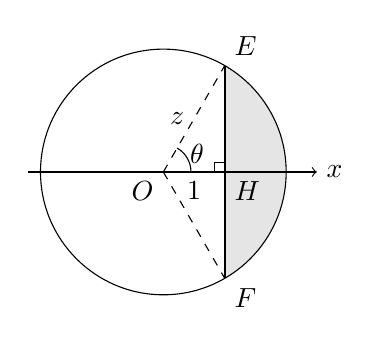
\begin{tikzpicture}[scale=0.78]
                 \fill[gray!20] (1,{-sqrt(3)}) arc[start angle=-60,end angle=60,radius=2] -- cycle;
                 \draw (0,0) circle[radius=2];
                 \draw[thick] (1,{-sqrt(3)}) -- (1,{sqrt(3)});
                 \draw[dashed] (0,0) -- (1,{sqrt(3)}) node[midway,left] {$z$};
                 \draw[dashed] (0,0) -- (1,{-sqrt(3)});
                 \draw[->] (-2.2,0) -- (2.5,0) node[right] {$x$};
                 \draw (0.45,0) arc[start angle=0,end angle=60,radius=0.45];
                 \node at (0.55,0.30) {$\theta$};
                 \node[below left] at (0,0) {$O$};
                 \node[below right] at (1,0) {$H$};
                 \node[above right] at (1,{sqrt(3)}) {$E$};
                 \node[below right] at (1,{-sqrt(3)}) {$F$};
                 \node[below] at (0.5,0) {$1$};
                 \draw (0.84,0) -- (0.84,0.16) -- (1,0.16);
                \end{tikzpicture}
      \BookFigureCaption{立体の水平断面と円弧・弦}
                \end{center}
                その面積を$A(z)$とすると,扇形から三角形を引いて,
                \[
                 \begin{aligned}
                 A(z)&=\frac12z^2\cdot2\theta
                      -\frac12\cdot2\sqrt{z^2-1}\cdot1\\
                     &=z^2\theta-\sqrt{z^2-1}.
                 \end{aligned}
                \]
                よって体積は$V=\int_1^2 A(z)\,dz$である.
                \,$\displaystyle z=\frac{1}{\cos\theta}$と置けば,
                \[
                 \sqrt{z^2-1}=\tan\theta,
                 \qquad dz=\frac{\sin\theta}{\cos^2\theta}\,d\theta.
                \]
                したがって,
                \[
                 \begin{aligned}
                 V&=\int_0^{\frac{\pi}{3}}\frac{\theta\sin\theta}{\cos^4\theta}\,d\theta\\
                  &\quad-\int_0^{\frac{\pi}{3}}\frac{\sin^2\theta}{\cos^3\theta}\,d\theta.
                 \end{aligned}
                \]
                第一項では$\displaystyle (\cos^{-3}\theta)'=\frac{3\sin\theta}{\cos^4\theta}$を使って部分積分する.
                第二項では$\sin^2\theta=1-\cos^2\theta$を使うと,
                \[
                 \begin{aligned}
                 V&=\left[\frac{\theta}{3\cos^3\theta}\right]_0^{\frac{\pi}{3}}
                      -\frac13I_3-(I_3-I_1)\\
                  &=\frac{8\pi}{9}-\frac43I_3+I_1\\
                  &=\frac{8\pi}{9}-\frac{4\sqrt3}{3}
                      +\frac13\log(2+\sqrt3).
                 \end{aligned}
                \]
                断面の半径と切断位置の関係を角度で表すと,最初に調べた$I_3$が自然に現れた.
                積分の\bookterm{recurrence}{漸化式}は\bookterm{sequence}{数列}だけの技法ではなく,図形から生まれる積分を計算するためにも使える.
          % F6: 一般項を求めずに減衰の速さを決める
          \item 分母に$a_n$があるが,本編の分数型と違って分母が二乗になっている.
                まず逆数を取って,\bookterm{general}{一般項}が求められるかだけでなく,増え方を評価できるかを調べる.
                \par\noindent
                \textbf{(1) 逆数の\bookterm{difference}{階差}を足す.}
                $a_1=1>0$であり,$a_n>0$なら$(1+2a_n)^2>0$なので$a_{n+1}>0$である.
                よって\bookterm{induction}{数学的帰納法}からすべての項が正で,$\displaystyle b_n=\frac{1}{a_n}$も定義できる.
                逆数を取ると,
                \[
                 \begin{aligned}
                 b_{n+1}&=\frac{(1+2a_n)^2}{a_n}\\
                         &=b_n+4+4a_n.
                 \end{aligned}
                \]
                したがって$b_{n+1}-b_n=4+4a_n>4$である.
                \,$k=1,\ldots,n-1$について足すと,
                \[
                 b_n-b_1=4(n-1)+4\sum_{k=1}^{n-1}a_k.
                \]
                $b_1=1$より,
                \[
                 b_n=4n-3+4\sum_{k=1}^{n-1}a_k.
                \]
                $n\geq2$なら右辺の総和は正だから,$b_n>4n-3$となる.
                ここまでの変形は,逆数化したあとに\bookterm{difference}{階差}を総和する本編の技法である.
                ただし総和に$a_k$が残っているため,この式だけでは\bookterm{general}{一般項}は得られていない.
                \par\noindent
                \textbf{(2) 項の収束と平均.}
                正の数の逆数を取ると不等号が逆向きになるので,
                \[
                 0<a_n<\frac1{4n-3}\qquad(n\geq2).
                \]
                挟み撃ちの原理より$a_n\to0$である.
                しかし平均にも$n$が入っているので,項の\bookterm{limit}{極限}だけで終えず,平均を直接評価する.
                任意の正数$\varepsilon$を取る.
                \,$a_n\to0$より,$k\geq N$なら$0<a_k<\varepsilon$となる正整数$N$が存在する.
                \,$C=\sum_{k=1}^{N-1}a_k$と置けば,$C$は$n$によらない定数である.
                \,$n\geq N$のとき,
                \[
                 \begin{aligned}
                 0<\frac1n\sum_{k=1}^{n}a_k
                 &=\frac Cn+\frac1n\sum_{k=N}^{n}a_k\\
                 &\leq\frac Cn+\frac{n-N+1}{n}\varepsilon\\
                 &\leq\frac Cn+\varepsilon.
                 \end{aligned}
                \]
                十分大きい$n$では$\displaystyle \frac{C}{n}<\varepsilon$でもあるため,平均は$2\varepsilon$より小さい.
                \,$\varepsilon$はいくらでも小さく取れるので,
                \[
                 \lim_{n\to\infty}\frac1n\sum_{k=1}^{n}a_k=0.
                \]
                この証明では,大きかった最初の有限個の項の影響は$n$で割ると消え,
                残りの項はすべて小さい,という二つの点を使っている.
                \par\noindent
                \textbf{(3) 逆数から減り方を読む.}
                (1)の等式を$n$で割ると,
                \[
                 \frac{b_n}{n}=4-\frac3n+
                            \frac4n\sum_{k=1}^{n-1}a_k.
                \]
                (2)より,
                \[
                 0\leq\frac1n\sum_{k=1}^{n-1}a_k
                 \leq\frac1n\sum_{k=1}^{n}a_k\longrightarrow0.
                \]
                したがって$\displaystyle \frac{b_n}{n}\to4$であり,
                \[
                 na_n=\cfrac{1}{\frac{b_n}{n}}\longrightarrow\frac14.
                \]
                \par
                最初に求めた上界は,$a_n\to0$を示すための中間結果である.
                それによって\bookterm{difference}{階差}の追加項$4a_n$の平均が消え,$b_n$は最終的に$4n$と同じ割合で増えると分かった.
                結論$\displaystyle na_n\to\frac{1}{4}$は,$a_n$の減少の速さが$\displaystyle \frac{1}{4n}$のそれに近づくことを表す.
                このように,\bookterm{general}{一般項}を閉じた式で表さなくても,\bookterm{recurrence}{漸化式}から\bookterm{sequence}{数列}の主要な性質を決められる.
          % F7: 1往復で整列できる札の配置
          \item \textbf{(1)~小さい例と左端の札.}
                  二枚ならすべて成功して$c_2=2$となる.
                  三枚では往路で$3$が右端へ移り,復路の最後に残り二枚が昇順になるので$c_3=6$である.
                  一般に最初の比較後,左端には$b=\min(A_1,A_2)$が残る.
                  その後でこの札に触れるのは復路の最後だけだから,最終位置は左から一番目か二番目である.
                  成功配置では$b\le2$が必要だが,これだけでは十分でない.
                  \smallskip\textbf{(2)~札を戻せる対応.}
                  数字を小さい順に読み替えても,比較・交換の動きは変わらない.
                  (1)により成功配置を次の四種類に分ける.
                  \[
                  \begin{array}{ll}
                    \text{\textcircled{1}}&A_1=1,\\
                    \text{\textcircled{2}}&A_2=1,\\
                    \text{\textcircled{3}}&A_1=2,\ A_2\ge3,\\
                    \text{\textcircled{4}}&A_2=2,\ A_1\ge3.
                  \end{array}
                  \]
                  \textbf{\textcircled{1},\textcircled{2}の数え方.}
                  最初の比較後に左端にある$1$を除くと,残る$n-1$枚への操作は小さい問題と同じになる.
                  復路の最後の$1$との比較は交換を起こさないので,成否も一致する.
                  逆に数字をすべて$1$増やし,$1$を先頭または二番目へ挿入すれば一意に戻せる.
                  よって各種類は$c_{n-1}$通りである.
                  \par\textbf{\textcircled{3}の数え方.}
                  先頭の$2$を除き,$1$はそのまま,$3,\ldots,n$を$2,\ldots,n-1$に読み替える.
                  縮約先の先頭は$1$でない.
                  例えば$(2,4,3,1)$は$(3,2,1)$に対応し,操作は次のようになる.
                  \[
                  \begin{array}{c|c|c}
                    &\text{元の配置}&\text{縮約配置}\\ \hline
                    \text{開始}&(2,4,3,1)&(3,2,1)\\
                    \text{往路後}&(2,3,1,4)&(2,1,3)\\
                    \text{復路後}&(1,2,3,4)&(1,2,3)
                  \end{array}
                  \]
                  \BookMathLayout{一般にも往路後の元の配列は$(2,B_1,\ldots,B_{n-1})$で,後ろの札への操作は縮約問題と同じである.}{一般にも往路後の元の配列は\newline
                  $(2,B_1,\ldots,B_{n-1})$で,後ろの札への操作は縮約問題と同じである.}
                  復路では最小の札$1$がその部分の左端へ移るため,最後の比較直前には
                  $(2,1,D_2,\ldots,D_{n-1})$となる.
                  最後の$(2,1)$を交換すれば,元の成否と縮約先の成否が一致する.
                  逆に,先頭が$1$でない成功配置で数字$2$以上を$1$増やし,先頭に$2$を戻せば一意に復元できる.
                  先頭が$1$の成功配置は\textcircled{1}の対応から$c_{n-2}$通りなので,
                  \textcircled{3}は$c_{n-1}-c_{n-2}$通りとなる.
                  \par\textbf{\textcircled{4}の数え方.}
                  最初の二枚を交換すれば\textcircled{3}に一対一で対応し,最初の比較後は同じ配列になる.
                  よってこちらも$c_{n-1}-c_{n-2}$通りであり,
                  \[
                    c_n=2c_{n-1}+2(c_{n-1}-c_{n-2})
                       =4c_{n-1}-2c_{n-2}.
                  \]
                  引いた$c_{n-2}$は,\textcircled{3}の縮約先から除く「先頭が$1$の配置」の数である.
                  \smallskip\textbf{(3)~個数から3項型へ.}
                  \bookterm{characteristic}{特性方程式}$x^2-4x+2=0$の根は$2\pm\sqrt2$である.
                  \[
                    c_n=P(2+\sqrt2)^{n-1}+Q(2-\sqrt2)^{n-1}
                  \]
                  に$c_1=1,c_2=2$を入れると$P=Q=1/2$であり,解答の式を得る.
                  $c_4=20,c_5=68$となる.二つのべきで$\sqrt2$の奇数次の項が相殺され,個数は整数になる.
                  この問の中心は,解く前の「何を取り除き,どう戻すか」という設計にある.
          % F8: 巨大な項の整除と, 添字の互除法
          \item \textbf{(1)~余りの\bookterm{recurrence}{漸化式}.}\par\nobreak
                  項は$1,2,5,26,677,\ldots$と急増するが,法$5$で余りの更新を追えば,
                  \[
                    1\longmapsto2\longmapsto0\longmapsto1
                  \]
                  と繰り返す.同じ余りから次は一意に決まるため,$5$の倍数となるのは$n=3,6,9,\ldots$である.
                  \smallskip\textbf{(2)~項を法に取る.}
                  $a_0=0$を補えば更新は$n\ge0$で使える.正整数$m$を固定すると,
                  \[
                    a_{m+j}\equiv a_j\pmod{a_m}\quad(j\ge0)
                  \]
                  が成り立つ.$j=0$では両辺が零であり,次も$a_{m+j}^2+1\equiv a_j^2+1$なので,
                  \bookterm{induction}{数学的帰納法}で示せる.
                  $n=qm+r$（$0\le r<m$）としてこの合同式を繰り返すと,
                  $a_n\equiv a_r\pmod{a_m}$となる.
                  また$a_{n+1}-a_n=a_n(a_n-1)+1>0$より$a_0$から厳密に増加するので,
                  $0\le a_r<a_m$かつ$a_r=0$は$r=0$の場合だけである.
                  よって,
                  \[
                    \begin{aligned}
                    a_m\mid a_n&\ \Longleftrightarrow\ a_r=0\\
                      &\ \Longleftrightarrow\ r=0\ \Longleftrightarrow\ m\mid n.
                    \end{aligned}
                  \]
                  $m=1$でも$r=0$なので成り立つ.(1)は$a_3=5$を用いた$m=3$の場合に当たる.
                  \smallskip\textbf{(3)~項から添字の互除法へ.}
                  $a_n-a_r$は$a_m$の倍数なので,共通の約数は変わらず,
                  \[
                    \gcd(a_m,a_n)=\gcd(a_m,a_r).
                  \]
                  \BookMathLayout{添字の互除法に沿って進むと,$d=\gcd(m,n)$と$0$で終わるため,}{添字の互除法に沿って進むと,\newline
                  $d=\gcd(m,n)$と$0$で終わるため,}
                  \[
                    \gcd(a_m,a_n)=\gcd(a_d,a_0)=a_d.
                  \]
                  最後は$a_0=0$と$\gcd(x,0)=x$を使った.
                  例では$3040=2026+1014$, $2026=1014+1012$, $1014=1012+2$, $1012=506\cdot2$より$d=2$である.
                  したがって$\gcd(a_{2026},a_{3040})=a_2=2$となる.
                  巨大な項どうしの整除関係を,小さな添字の計算へ移せた.
          % F9: 整数方程式の解を生み出す漸化式
          \item \textbf{(1)~一つの解から次の解へ.}
                  $9+y^2+z^2=3yz$を$y$の二次方程式と見ると,もう一つの根は$3z-y$である.
                  実際,
                  \[
                    \begin{aligned}
                    &9+z^2+(3z-y)^2-3z(3z-y)\\
                    &\qquad=9+y^2+z^2-3yz=0.
                    \end{aligned}
                  \]
                  $3z-y$は整数で,$0<y\le z$より$3z-y\ge2z>z>0$となる.
                  新しい二項も大小関係を満たすため,操作を繰り返せる.
                  \smallskip\textbf{(2)~整数解を\bookterm{sequence}{数列}にする.}
                  $(3,3,3)$からの操作で,$y,z$は$(3,3),(3,6),(6,15),(15,39),\ldots$と変わる.
                  隣接する値を$u_n,u_{n+1}$とすれば$u_{n+2}=3u_{n+1}-u_n$となる.
                  \bookterm{characteristic}{特性方程式}$t^2-3t+1=0$の根を$\alpha,\beta$とし,
                  $u_n=P\alpha^n+Q\beta^n$とおく.
                  $u_0=u_1=3$から,
                  \[
                    P=\frac{3(\sqrt5-1)}{2\sqrt5},\quad
                    Q=\frac{3(\sqrt5+1)}{2\sqrt5}
                  \]
                  となり,解答の式を得る.
                  \smallskip\textbf{(3)~整数性と方程式の確認.}
                  初期値と更新の係数から全項が整数である.
                  $u_2=6>u_1=3$であり,$u_{n+1}>u_n>0$なら$u_{n+2}>2u_{n+1}>u_{n+1}$となるため,
                  $n\ge1$で正値と厳密な増加が続く.
                  隣接する二項から作る
                  \[
                    I_n=u_n^2+u_{n+1}^2-3u_nu_{n+1}
                  \]
                  に更新式を入れると,
                  \[
                  \begin{aligned}
                    I_{n+1}&=u_{n+1}^2+(3u_{n+1}-u_n)^2\\
                           &\quad-3u_{n+1}(3u_{n+1}-u_n)=I_n.
                  \end{aligned}
                  \]
                  よって$I_n=I_0=-9$から$(3,u_n,u_{n+1})$は正の整数解となる.
                  増加するため解は互いに異なり,無限個得られる.ここでは全解の分類まではしていない.
                  最後に$0<\beta<1<\alpha$と$P,Q>0$から,
                  \[
                    \frac{u_{n+1}}{u_n}
                      =\alpha\,\cfrac{P+Q(\frac\beta\alpha)^{n+1}}
                                       {P+Q(\frac\beta\alpha)^n}
                      \longrightarrow\alpha.
                  \]
                  更新式は整数性を保証し,\bookterm{general}{一般項}は整数の比が近づく無理数を示している.
          % F10: 元のペアをすべて解消する組み替え
          \item \textbf{(1) 小さい場合を数える.}
                  $n=1$では相手がいないので$S(1)=0$である.
                  $n=2$では$(A_1,B_2),(A_2,B_1)$の一通り,
                  $n=3$では相手の添字が$(2,3,1),(3,1,2)$の二通りである.
                  $S(0)=1$は「何も作らない組合せ」を一通りと数える約束である.
                  \par\smallskip\textbf{(2) 相手を決めて分ける.}
                  $A_1$の相手$B_j$を$j\ne1$の$n-1$通りから選び,固定する.
                  $A_j$の相手が$B_1$なら,四要素を除いた$n-2$組を完全に組み替える$S(n-2)$通りである.
                  そうでない場合,$B_1$の相手を$A_k$（$k\ne1,j$）とする.
                  \[
                    (A_1,B_j),(A_k,B_1)\ \longmapsto\ (A_k,B_j)
                  \]
                  として$A_1,B_1$を除けば,添字$2,\ldots,n$の完全な組み替えになる.
                  $k\ne j$なので元のペアは増えない.
                  逆に$B_j$の相手$A_k$を見つけて二組へ戻せば,一意に復元できる.
                  この一対一対応から後者は$S(n-1)$通りであり,
                  \[
                    S(n)=(n-1)\{S(n-1)+S(n-2)\}.
                  \]
                  \par\smallskip\textbf{(3) 差と階乗で整理する.}
                  係数が$n$で変わるため,\bookterm{constant}{定数係数}の特性方程式は使えない.
                  $T_n=S(n)-nS(n-1)$とおくと,$n\ge2$で,
                  \[
                    T_n=(n-1)S(n-2)-S(n-1)=-T_{n-1}.
                  \]
                  $T_1=-1$から$T_n=(-1)^n$となる.
                  $S(n)=nS(n-1)+(-1)^n$の倍率を階乗へ吸収し,$P_n=S(n)/n!$とおけば,
                  \[
                    P_n-P_{n-1}=\frac{(-1)^n}{n!},\quad P_0=1.
                  \]
                  \bookterm{difference}{階差}を足すと,
                  \[
                    S(n)=n!\sum_{k=0}^n\frac{(-1)^k}{k!}.
                  \]
                  $S(4)=9,S(5)=44$となる.
                  等比型,\bookterm{ratio}{階比}による\bookterm{normalize}{正規化},\bookterm{difference}{階差}型を順に使った.
                  \par\smallskip\textbf{(4) 残る組数で数える.}
                  残す$r$組を選び,残りを完全に組み替えれば$\binom nrS(n-r)$通りである.
                  残るペアは完成形から一意に決まり,$r=n$も$S(0)=1$によって含む.
                  平均には,固定した元のペアが残る$(n-1)!$通りを$n$組分数える.
                  $r$組残る配置は$r$回数えられるので,残る組数の合計は$n(n-1)!$であり,平均は$n(n-1)!/n!=1$となる.
                  \par\smallskip\noindent\textbf{【確率として読む】}\par\nopagebreak[4]
                  元の位置に戻る要素のない並べ替えを\textbf{完全順列（錯置）}という.
                  全$n!$通りが等確率なら,元のペアが一組も残らない確率は,
                  \[
                    P_n=\frac{S(n)}{n!}=\sum_{k=0}^n\frac{(-1)^k}{k!}.
                  \]
                  階乗で割る操作は,\textbf{個数を確率に直す操作}でもある.
                  \par\smallskip\noindent\textbf{【偶奇に分けて極限を確かめる】}\par\nopagebreak[4]
                  まず収束を示し,その後で値を決める.無限級数展開は仮定せず,
                  \bookterm{binomial}{二項定理}と\sectionref*{節：対数}の$e$の定義を使う.
                  \[
                  \begin{aligned}
                    P_{2m+2}-P_{2m}&=-\frac{2m+1}{(2m+2)!}<0,\\
                    P_{2m+3}-P_{2m+1}&=\frac{2m+2}{(2m+3)!}>0,\\
                    P_{2m}-P_{2m+1}&=\frac1{(2m+1)!}\longrightarrow0.
                  \end{aligned}
                  \]
                  偶数番目は減少,奇数番目は増加し,確率は$0$以上$1$以下である.
                  よって両者は共通の\bookterm{limit}{極限}$L$をもつ.
                  \par\smallskip\noindent\textbf{【二項定理で極限の値を決める】}\par\nopagebreak[4]
                  整数$M\ge2$について$b_{M,k}=\binom Mk/M^k$とおくと,
                  \[
                    \frac{b_{M,k+1}}{b_{M,k}}=\frac{M-k}{M(k+1)}\le1
                    \quad(0\le k<M).
                  \]
                  有限の二項展開を途中で止め,残りを隣り合う二項ずつ組にする.
                  奇数で止めた残りは非負,偶数で止めた残りは非正なので,$M\ge2\ell+1$では,
                  \[
                  \begin{aligned}
                    \sum_{k=0}^{2\ell+1}(-1)^kb_{M,k}
                      &\le\left(1-\frac1M\right)^M,\\
                    \left(1-\frac1M\right)^M
                      &\le\sum_{k=0}^{2\ell}(-1)^kb_{M,k}.
                  \end{aligned}
                  \]
                  \textbf{まず$\ell$を固定して$M\to\infty$とする.}
                  和の項数は固定され,各項で,
                  \[
                    b_{M,k}=\frac1{k!}\prod_{j=0}^{k-1}\left(1-\frac jM\right)
                      \longrightarrow\frac1{k!}
                  \]
                  となる.$k=0$の空積は$1$である.
                  一方,$t=M-1$とおくと,
                  \[
                    \left(1-\frac1M\right)^M=\left(1+\frac1t\right)^{-t-1}
                      \longrightarrow\frac1e
                  \]
                  である.$(1+1/t)^t\to e$と$1+1/t\to1$を使った.
                  したがって$P_{2\ell+1}\le1/e\le P_{2\ell}$となる.
                  \textbf{次に$\ell\to\infty$とする.}両端が$L$へ近づくため,
                  \[
                    \boxed{\lim_{n\to\infty}\frac{S(n)}{n!}=\frac1e\simeq0.368}.
                  \]
                  \par\smallskip\noindent\textbf{【個数はどこまで近いか】}\par\nopagebreak[4]
                  偶奇の各列が厳密に進むので,$1/e$は隣り合う$P_n,P_{n+1}$の間に厳密に入る.
                  よって$n\ge1$で,
                  \[
                  \begin{aligned}
                    \left|P_n-\frac1e\right|&<\frac1{(n+1)!},\\
                    \left|S(n)-\frac{n!}e\right|&<\frac1{n+1}\le\frac12.
                  \end{aligned}
                  \]
                  下段は上段を$n!$倍したものであり,$S(n)$は$n!/e$に最も近い整数となる.
                  数え上げの\bookterm{recurrence}{漸化式}が,階乗・確率・自然\bookterm{logarithm}{対数}の底を結んだ.
        \end{enumerate}

    \subsection{発展・特殊型}\label{節：発展パターン・特殊性質型の演習}
      ここでは,\sectionref{節：発展パターン}と\sectionref{節：特殊性質型}で扱った\bookterm{recurrence}{漸化式}を,\,15題で練習する.
      \bookterm{floor}{ガウス記号}では整数性や余り,多項間の関係では\bookterm{difference}{階差}や\bookterm{characteristic}{特性方程式},
      \bookterm{nonlinear}{非線形}な式では対称式や\bookterm{trigonometric}{三角関数}の恒等式が手掛かりになる.
      まず式のどの部分に着目したかを述べ,置換や場合分けを選ぼう.
      \bookterm{general}{一般項}の候補が見つかったら,\bookterm{initial}{初期条件}と\bookterm{recurrence}{漸化式}をともに満たすことを確認する.
      分数式では分母,\bookterm{trigonometric}{三角関数}では角度の定義域も確かめてほしい.
      問14・問15では初項を動かし,定\bookterm{sequence}{数列}・周期列・有界な\bookterm{sequence}{数列}が現れる条件を調べる.
      以下,特に指定しない限り,\,$\displaystyle n$は正の整数とする.
      $\displaystyle \lfloor x\rfloor$は$\displaystyle x$を超えない最大の整数を表す.
      周期の最小値とは,すべての添字で$\displaystyle a_{n+p}=a_n$となる正の整数$\displaystyle p$の最小値をいう.

      \subsubsection{問題}\label{節：発展パターン・特殊性質型の演習：問題}
        \begin{enumerate}[label=\textbf{問\arabic*.},leftmargin=3.8em,format=\bookitemlink{practice-special}{problem}{answer}]
          % E1: ガウス型・整数の半減
          \item \bookterm{sequence}{数列}$\displaystyle \{a_n\}$を
                \[
                  a_1=2026,\qquad
                  a_{n+1}=\left\lfloor\frac{a_n}{2}\right\rfloor
                \]
                によって定める.
                \par\smallskip\noindent
                (1) \bookterm{general}{一般項}を求めよ.
                \par\smallskip\noindent
                (2) 初めて$\displaystyle a_n=0$となる添字$\displaystyle n$を求めよ.
          % E2: ガウス型・三つずつの群
          \item \bookterm{sequence}{数列}$\displaystyle \{a_n\}$を
                \[
                  a_0=0,\qquad
                  a_{n+1}=a_n+\left\lfloor\frac{n+1}{3}\right\rfloor
                  \quad(n\ge0)
                \]
                によって定める.\,
                $\displaystyle n=3q+r$（$\displaystyle q\ge0$,\,$\displaystyle r=0,1,2$）とおき,
                \bookterm{general}{一般項}を$\displaystyle q,r$で表せ.
          % E3: ガウス型・余りの有限個の状態
          \item \bookterm{sequence}{数列}$\displaystyle \{a_n\}$を
                \[
                  a_1=1,\qquad
                  a_{n+1}=2a_n+1
                    -5\left\lfloor\frac{2a_n+1}{5}\right\rfloor
                \]
                によって定める.
                \par\smallskip\noindent
                (1) すべての項が$\displaystyle 0,1,2,3,4$のいずれかになることを示せ.
                \par\smallskip\noindent
                (2) \bookterm{general}{一般項}を,\,$\displaystyle n$を$\displaystyle 4$で割った余りで場合分けして表せ.
                また,周期の最小値を求めよ.
          % E4: 隣接4項間・三階差が定数
          \item \bookterm{sequence}{数列}$\displaystyle \{a_n\}$を
                \[
                  a_1=2,\qquad a_2=9,\qquad a_3=28,
                \]
                \[
                  a_{n+3}=3a_{n+2}-3a_{n+1}+a_n+6
                \]
                によって定める.
                \par\smallskip\noindent
                (1) $\displaystyle d_n=a_{n+2}-2a_{n+1}+a_n$とおき,\,$\displaystyle d_n$を求めよ.
                \par\smallskip\noindent
                (2) \bookterm{general}{一般項}を求めよ.
          % E5: 隣接4項間・異なる三つの特性根
          \item \bookterm{sequence}{数列}$\displaystyle \{a_n\}$を
                \[
                  a_1=3,\qquad a_2=6,\qquad a_3=14,
                \]
                \[
                  a_{n+3}=6a_{n+2}-11a_{n+1}+6a_n
                \]
                によって定める.
                \par\smallskip\noindent
                (1) $\displaystyle d_n=a_{n+2}-3a_{n+1}+2a_n$とおき,\,$\displaystyle d_n$を求めよ.
                \par\smallskip\noindent
                (2) \bookterm{general}{一般項}を求めよ.
          % E6: 虚数解型・周期6
          \item \bookterm{sequence}{数列}$\displaystyle \{a_n\}$を
                \[
                  a_1=0,\qquad a_2=1,\qquad
                  a_{n+2}=a_{n+1}-a_n
                \]
                によって定める.
                \par\smallskip\noindent
                (1) \bookterm{trigonometric}{三角関数}を用いて\bookterm{general}{一般項}を表せ.
                \par\smallskip\noindent
                (2) 周期の最小値を求めよ.
          % E7: 虚数解型・振幅が減衰する数列
          \item \bookterm{sequence}{数列}$\displaystyle \{a_n\}$を
                \[
                  a_1=1,\qquad a_2=0,\qquad
                  a_{n+2}=a_{n+1}-\frac12a_n
                \]
                によって定める.\bookterm{trigonometric}{三角関数}を用いて\bookterm{general}{一般項}を表し,
                $\displaystyle \lim_{n\to\infty}a_n$を求めよ.
          % E8: 非隣接2項間・奇数列と偶数列の逆数
          \item \bookterm{sequence}{数列}$\displaystyle \{a_n\}$を
                \[
                  a_1=1,\qquad a_2=2,\qquad
                  a_{n+2}=\frac{a_n}{1+a_n}
                \]
                によって定める.
                \par\smallskip\noindent
                (1) すべての項が正であることを示し,
                $\displaystyle a_{2k-1},a_{2k}$を$\displaystyle k$で表せ.
                ただし,\,$\displaystyle k$は正の整数とする.
                \par\smallskip\noindent
                (2) $\displaystyle \lim_{n\to\infty}a_n$を求めよ.
          % E9: 基本対称式型・平行移動して恒等式を使う
          \item \bookterm{sequence}{数列}$\displaystyle \{a_n\}$を
                \[
                  a_1=\frac72,\qquad
                  a_{n+1}=a_n^2-2a_n
                \]
                によって定める.
                \par\smallskip\noindent
                (1) $\displaystyle b_n=a_n-1$とおき,\,$\displaystyle b_n$の\bookterm{recurrence}{漸化式}を求めよ.
                \par\smallskip\noindent
                (2) 恒等式
                \[
                  \left(u+u^{-1}\right)^2-2=u^2+u^{-2}
                  \quad(u\ne0)
                \]
                を用いて$\displaystyle a_n$の\bookterm{general}{一般項}を求めよ.
          % E10: 基本対称式型・三乗の対称式
          \item \bookterm{sequence}{数列}$\displaystyle \{a_n\}$を
                \[
                  a_1=\frac52,\qquad
                  a_{n+1}=a_n^3-3a_n
                \]
                によって定める.
                \par\smallskip\noindent
                (1) 恒等式
                \[
                  \left(u+u^{-1}\right)^3
                  -3\left(u+u^{-1}\right)=u^3+u^{-3}
                \]
                を示せ.ただし,\,$\displaystyle u\ne0$とする.
                \par\smallskip\noindent
                (2) \bookterm{general}{一般項}を求めよ.
          % E11: 三角関数型・余弦の倍角と周期3
          \item \bookterm{sequence}{数列}$\displaystyle \{a_n\}$を
                \[
                  a_1=\cos\frac{2\pi}{7},\qquad
                  a_{n+1}=2a_n^2-1
                \]
                によって定める.
                \par\smallskip\noindent
                (1) \bookterm{general}{一般項}を求めよ.
                \par\smallskip\noindent
                (2) 周期の最小値を求めよ.
          % E12: 三角関数型・正接の定義域と周期4
          \item 初項と次の項を計算する規則を
                \[
                  a_1=\tan\frac{\pi}{5},\qquad
                  a_{n+1}=\frac{2a_n}{1-a_n^2}
                \]
                とする.
                \par\smallskip\noindent
                (1) \bookterm{general}{一般項}の候補を求め,すべての段階で分母が$\displaystyle 0$にならず,
                \bookterm{sequence}{数列}が定義できることを示せ.
                \par\smallskip\noindent
                (2) 周期の最小値を求めよ.
          % E13: ニュートン法型・初項が収束先より小さい場合
          \item \bookterm{sequence}{数列}$\displaystyle \{a_n\}$を
                \[
                  a_1=1,\qquad
                  a_{n+1}=\frac{a_n^2+3}{2a_n}
                \]
                によって定める.
                \par\smallskip\noindent
                (1) すべての項が正であることを示せ.
                \par\smallskip\noindent
                (2) $\displaystyle b_n=\frac{a_n-\sqrt3}{a_n+\sqrt3}$とおき,
                $\displaystyle b_n,a_n$の\bookterm{general}{一般項}を求めよ.
                \par\smallskip\noindent
                (3) $\displaystyle n\ge2$で$\displaystyle a_n>\sqrt3$かつ
                $\displaystyle a_{n+1}<a_n$であることを示し,\,$\displaystyle \lim_{n\to\infty}a_n$を求めよ.
          % E14: 初項依存型・不動点と2周期点
          \item 実数$\displaystyle c$を初項として,\bookterm{sequence}{数列}$\displaystyle \{a_n\}$を
                \[
                  a_1=c,\qquad a_{n+1}=a_n^2-1
                \]
                によって定める.
                \par\smallskip\noindent
                (1) \bookterm{sequence}{数列}が定\bookterm{sequence}{数列}となる$\displaystyle c$をすべて求めよ.
                \par\smallskip\noindent
                \BookMathLayout{(2) 定\bookterm{sequence}{数列}ではなく,すべての$\displaystyle n$で$\displaystyle a_{n+2}=a_n$を満たす
                $\displaystyle c$をすべて求め,それぞれの場合の\bookterm{general}{一般項}を表せ.}{(2) 定\bookterm{sequence}{数列}ではなく,\\すべての$\displaystyle n$で$\displaystyle a_{n+2}=a_n$を満たす
                $\displaystyle c$をすべて求め,それぞれの場合の\bookterm{general}{一般項}を表せ.}
          % E15: 初項依存型・有界になる初項の範囲
          \item 実数$\displaystyle c$を初項として,\bookterm{sequence}{数列}$\displaystyle \{a_n\}$を
                \[
                  a_1=c,\qquad a_{n+1}=a_n^2-2
                \]
                によって定める.
                \par\smallskip\noindent
                (1) $\displaystyle c=-2,-1,0,2$のそれぞれについて,最初の4項を求めよ.
                \par\smallskip\noindent
                (2) $\displaystyle -2\le c\le2$のとき,\,$\displaystyle c=2\cos\theta$
                （$\displaystyle 0\le\theta\le\pi$）とおき,\bookterm{general}{一般項}を求めよ.
                また,すべての項が$\displaystyle -2$以上$\displaystyle 2$以下であることを示せ.
                \par\smallskip\noindent
                (3) $\displaystyle |c|>2$のとき,\,$\displaystyle a_n\to+\infty$を示せ.
                以上から,\bookterm{sequence}{数列}が有界となる$\displaystyle c$の範囲を求めよ.
        \end{enumerate}

      \subsubsection{方針}\label{節：発展パターン・特殊性質型の演習：方針}
        \begin{enumerate}[label=\textbf{問\arabic*.},leftmargin=3.8em,format=\bookitemlink{practice-special}{hint}{problem}]
          % E1
          \item 整数を$\displaystyle 2$で割った商と余りに分け,
                $\displaystyle \left\lfloor\frac{\lfloor x\rfloor}{2}\right\rfloor
                =\left\lfloor\frac{x}{2}\right\rfloor$となることを確かめる.
                初めて$\displaystyle 0$になる位置は,\,$\displaystyle 2026$と$\displaystyle 2$の累乗を比べればよい.
          % E2
          \item \bookterm{difference}{階差}を足すと$\displaystyle \sum_{k=1}^{n}\lfloor\frac{k}{3}\rfloor$になる.
                同じ値を取る添字を三つずつまとめ,最後の群を$\displaystyle r+1$項として数える.
          % E3
          \item $\displaystyle x-5\lfloor\frac{x}{5}\rfloor$は整数$\displaystyle x$を$\displaystyle 5$で割った余りである.
                項の値が五つに絞れたら,それぞれが次にどの値へ移るかを表にする.
          % E4
          \item $\displaystyle d_{n+1}-d_n$を作ると元の\bookterm{recurrence}{漸化式}の左辺が現れる.
                その後,\,$\displaystyle e_n=a_{n+1}-a_n$を求め,もう一度足して$\displaystyle a_n$へ戻す.
          % E5
          \item $\displaystyle d_{n+1}-3d_n$を展開すると$\displaystyle 0$になる.
                得られた3項間の式を満たす$\displaystyle 3^{n-1}$を引き,残りを解く.
          % E6
          \item \bookterm{characteristic}{特性方程式}の根の絶対値と\bookterm{argument}{偏角}を調べる.
                最初の二つの項に合う$\displaystyle \sin$の式を作り,実際の値の並びから周期を確かめる.
          % E7
          \item \bookterm{root}{特性根}の絶対値は$\displaystyle 1$未満である.
                \bookterm{polar}{極形式}から\bookterm{trigonometric}{三角関数}の\bookterm{general}{一般項}を作り,その絶対値を\bookterm{geometric}{等比数列}で上から押さえる.
          % E8
          \item 正値を確かめてから逆数を取る.
                奇数番目と偶数番目を別々の\bookterm{sequence}{数列}にすると,二つの\bookterm{arithmetic}{等差数列}が得られる.
          % E9
          \item $\displaystyle a_n^2-2a_n=(a_n-1)^2-1$と\bookterm{square}{平方完成}する.
                $\displaystyle b_1=2+2^{-1}$と書けば,恒等式によって指数が毎回2倍になる.
          % E10
          \item 展開すると,交差項が$\displaystyle 3(u+u^{-1})$であることが分かる.
                初項を$\displaystyle 2+2^{-1}$と表し,指数を毎回3倍にする候補を作る.
          % E11
          \item 余弦の倍角公式で,角度を毎回2倍にする候補を作る.
                3回倍にした角度と元の角度との差が$\displaystyle 2\pi$の整数倍になることを調べる.
          % E12
          \item 正接の倍角公式を使う.
                候補の角度が$\displaystyle \frac{\pi}{2}$に$\displaystyle \pi$の整数倍を加えた値になるかを,
                整数の偶奇で判断する.次の角度でも正接が定義できれば,\bookterm{recurrence}{漸化式}の分母も$\displaystyle 0$にならない.
          % E13
          \item $\displaystyle a_{n+1}\pm\sqrt3$の分子は平方になる.比を取って$\displaystyle b_{n+1}=b_n^2$を導く.
                $\displaystyle b_1<0$なので,\bookterm{logarithm}{対数}を取らずにべき乗の形を帰納法で確かめる.
                減少を示す範囲が$\displaystyle n\ge2$であることにも注意する.
          % E14
          \item 定\bookterm{sequence}{数列}には$\displaystyle a_2=a_1$,周期2の候補には$\displaystyle a_3=a_1$が必要である.
                後者の方程式を因数分解し,定\bookterm{sequence}{数列}の初項を除く.残った初項が実際に二つの値を往復することも確かめる.
          % E15
          \item $\displaystyle |c|\le2$では$\displaystyle 2\cos\theta$という表示を使う.
                $\displaystyle |c|>2$では第2項が$\displaystyle 2$を超えるので,
                $\displaystyle a_{n+1}-2=(a_n-2)(a_n+2)$から下からの評価を作る.
        \end{enumerate}

      \subsubsection{答え}\label{節：発展パターン・特殊性質型の演習：解答}
        \begin{enumerate}[label=\textbf{問\arabic*.},leftmargin=3.8em,format=\bookitemlink{practice-special}{answer}{problem}]
          % E1
          \item (1)
                \[
                  a_n=\left\lfloor\frac{2026}{2^{n-1}}\right\rfloor.
                \]
                (2) $\displaystyle n=12$である.
          % E2
          \item
                \[
                  a_n=\frac{3q(q-1)}2+q(r+1),
                \]
                \[
                  n=3q+r,\qquad q\ge0,\quad r=0,1,2.
                \]
          % E3
          \item (1) 整数性と\bookterm{floor-function}{床関数}の定義から,各項は$\displaystyle 0$以上$\displaystyle 4$以下の整数となる.
                \par\smallskip\noindent
                (2) $\displaystyle k$を$\displaystyle 0$以上の整数として,
                \[
                  a_{4k+1}=1,\quad a_{4k+2}=3,
                \]
                \[
                  a_{4k+3}=2,\quad a_{4k+4}=0.
                \]
                周期の最小値は$\displaystyle 4$である.
          % E4
          \item (1) $\displaystyle d_n=6n+6$.
                \par\smallskip\noindent
                (2) $\displaystyle a_n=n^3+1$.
          % E5
          \item (1) $\displaystyle d_n=2\cdot3^{n-1}$.
                \par\smallskip\noindent
                (2)
                \[
                  a_n=1+2^{n-1}+3^{n-1}.
                \]
          % E6
          \item (1)
                \[
                  a_n=\frac2{\sqrt3}\sin\frac{(n-1)\pi}{3}.
                \]
                (2) 周期の最小値は$\displaystyle 6$である.
          % E7
          \item
                \[
                  a_n=\left(\frac1{\sqrt2}\right)^{n-1}
                    \left(\cos t_n-\sin t_n\right),
                \]
                \[
                  t_n=\frac{(n-1)\pi}{4},\qquad
                  \lim_{n\to\infty}a_n=0.
                \]
          % E8
          \item (1) すべての項は正であり,
                \[
                  a_{2k-1}=\frac1k,\qquad
                  a_{2k}=\frac2{2k-1}\quad(k\ge1).
                \]
                (2) \bookterm{limit}{極限}は$\displaystyle 0$である.
          % E9
          \item (1) $\displaystyle b_1=\frac52$,\,$\displaystyle b_{n+1}=b_n^2-2$.
                \par\smallskip\noindent
                (2)
                \[
                  a_n=1+2^{\,2^{n-1}}+2^{-2^{n-1}}.
                \]
          % E10
          \item (1) 左辺を展開すると右辺を得る.
                \par\smallskip\noindent
                (2)
                \[
                  a_n=2^{\,3^{n-1}}+2^{-3^{n-1}}.
                \]
          % E11
          \item (1)
                \[
                  a_n=\cos\left(2^{n-1}\frac{2\pi}{7}\right).
                \]
                (2) 周期の最小値は$\displaystyle 3$である.
          % E12
          \item (1)
                \[
                  a_n=\tan\left(2^{n-1}\frac{\pi}{5}\right).
                \]
                すべての項で正接が定義でき,\bookterm{recurrence}{漸化式}の分母も$\displaystyle 0$にならない.
                \par\smallskip\noindent
                (2) 周期の最小値は$\displaystyle 4$である.
          % E13
          \item (1) 初項が正で,正の項から次の正の項が定まる.
                \par\smallskip\noindent
                (2) $\displaystyle q=\sqrt3-2$とおくと,
                \[
                  b_n=q^{\,2^{n-1}},\qquad
                  a_n=\sqrt3\,\frac{1+q^{\,2^{n-1}}}{1-q^{\,2^{n-1}}}.
                \]
                (3) $\displaystyle n\ge2$で設問の二つの不等式が成り立ち,
                \[
                  \lim_{n\to\infty}a_n=\sqrt3.
                \]
          % E14
          \item (1)
                \[
                  c=\frac{1+\sqrt5}{2},\quad
                  \frac{1-\sqrt5}{2}.
                \]
                それぞれ$\displaystyle a_n=c$である.
                \par\smallskip\noindent
                (2) $\displaystyle c=0,-1$であり,どちらも
                \[
                  a_n=-\frac12+\left(c+\frac12\right)(-1)^{n-1}
                \]
                と表せる.周期の最小値は$\displaystyle 2$である.
          % E15
          \item (1)
                \[
                  \begin{array}{c|rrrr}
                    c&a_1&a_2&a_3&a_4\\ \hline
                    -2&-2&2&2&2\\
                    -1&-1&-1&-1&-1\\
                     0&0&-2&2&2\\
                     2&2&2&2&2
                  \end{array}
                \]
                (2)
                \[
                  a_n=2\cos(2^{n-1}\theta),\qquad -2\le a_n\le2.
                \]
                (3) $\displaystyle n\ge2$で
                \[
                  a_n\ge2+4^{n-2}(c^2-4)
                \]
                となり,\,$\displaystyle a_n\to+\infty$である.
                有界となる範囲は$\displaystyle -2\le c\le2$である.
        \end{enumerate}

      \subsubsection{解説}\label{節：発展パターン・特殊性質型の演習：解法}
        \begin{enumerate}[label=\textbf{問\arabic*.},leftmargin=3.8em,format=\bookitemlink{practice-special}{solution}{problem}]
          % E1
          \item \textbf{(1)~整数部分を分ける.}
                \sectionref{節：ガウス型}の整数性に着目する.
                非負の実数$\displaystyle x$について,整数$\displaystyle \lfloor x\rfloor$を
                \[
                  \lfloor x\rfloor=2q+r,\qquad r=0,1
                \]
                と表す.\bookterm{floor-function}{床関数}の定義を使って$\displaystyle 2$で割れば,
                \begin{align*}
                  \frac x2&\ge q+\frac r2\ge q,\\
                  \frac x2&<q+\frac{r+1}{2}\le q+1.
                \end{align*}
                したがって,
                \[
                  \left\lfloor\frac{x}{2}\right\rfloor=q
                    =\left\lfloor\frac{\lfloor x\rfloor}{2}\right\rfloor.
                \]
                $\displaystyle a_1=\lfloor2026\rfloor$であり,この恒等式を繰り返し使うと,
                \[
                  a_n=\left\lfloor\frac{2026}{2^{n-1}}\right\rfloor
                \]
                が帰納法で得られる.

                \smallskip
                \textbf{(2)~1未満になる位置.}
                $\displaystyle 2^{10}=1024\le2026<2048=2^{11}$だから,
                \[
                  a_{11}=1,\qquad a_{12}=0.
                \]
                $\displaystyle n\le11$では切り捨てる前の値が$\displaystyle 1$以上なので,
                初めて$\displaystyle 0$となるのは$\displaystyle n=12$である.
                毎回の切り捨てを一つの\bookterm{floor-function}{床関数}にまとめられる理由は,割る数が正の整数であることにある.
          % E2
          \item \textbf{同じ値をまとめて足す.}
                \sectionref{節：ガウス型}の群\bookterm{sequence}{数列}の見方を使う.
                \bookterm{difference}{階差}を足すと,
                \[
                  a_n=\sum_{k=1}^{n}\left\lfloor\frac{k}{3}\right\rfloor.
                \]
                $\displaystyle k=1,2$では値は$\displaystyle 0$である.
                正の整数$\displaystyle j$について,\,$\displaystyle k=3j,3j+1,3j+2$の三つで値が$\displaystyle j$になる.
                $\displaystyle n=3q+r$とおくと,\,$\displaystyle q\ge1$の場合,
                値が$\displaystyle 1,2,\ldots,q-1$となる群がすべてそろい,
                値が$\displaystyle q$となる最後の群が$\displaystyle r+1$項だけある.
                よって,
                \begin{align*}
                  a_n&=3\sum_{j=1}^{q-1}j+q(r+1)\\
                     &=\frac{3q(q-1)}2+q(r+1).
                \end{align*}
                $\displaystyle q=0$,すなわち$\displaystyle n=0,1,2$でも,
                実際の値とこの式の値はともに$\displaystyle 0$である.
                最後の群を常に三つとして数えると誤るので,余り$\displaystyle r$で途中までの項数を表している.
          % E3
          \item \textbf{(1)~余りに読み替える.}
                \sectionref{節：ガウス型}では,\bookterm{floor}{ガウス記号}が整数問題の道具にもなる.
                整数$\displaystyle x$について\bookterm{floor-function}{床関数}の定義から,
                \[
                  0\le x-5\left\lfloor\frac{x}{5}\right\rfloor<5.
                \]
                この値は整数だから$\displaystyle 0,1,2,3,4$のいずれかである.
                初項は整数であり,整数の項から次の整数の項が定まるので,
                $\displaystyle x=2a_n+1$として帰納法を使えばよい.

                \smallskip
                \textbf{(2)~五つの値の更新.}
                (1)より,次の表だけを調べれば十分である.
                \[
                  \begin{array}{c|rrrrr}
                    a_n&0&1&2&3&4\\ \hline
                    a_{n+1}&1&3&0&2&4
                  \end{array}
                \]
                初項$\displaystyle 1$からは$\displaystyle 1,3,2,0,1,\ldots$と進む.
                どの値からも次の値は一つに決まるため,この四つの値の繰り返しが帰納法で続く.
                よって解答の\bookterm{general}{一般項}を得る.
                最初の四つの値がすべて異なるので,周期の最小値は$\displaystyle 4$である.
                \bookterm{sequence}{数列}全体の大きさを追う代わりに,取り得る値を先に絞ったことが解法の鍵である.
          % E4
          \item \textbf{(1)~4項型から\bookterm{difference}{階差}へ.}
                \sectionref{節：隣接4項間漸化式型}と同じく,\bookterm{difference}{階差}の組合せを見る.
                設問の$\displaystyle d_n$について,
                \begin{align*}
                  d_{n+1}-d_n
                    &=a_{n+3}-3a_{n+2}\\
                    &\quad+3a_{n+1}-a_n\\
                    &=6.
                \end{align*}
                $\displaystyle d_1=28-2\cdot9+2=12$だから,
                \[
                  d_n=12+6(n-1)=6n+6.
                \]

                \smallskip
                \textbf{(2)~\bookterm{difference}{階差}を足して戻す.}
                $\displaystyle e_n=a_{n+1}-a_n$とおくと,
                \[
                  e_{n+1}-e_n=d_n=6n+6,
                \]
                かつ$\displaystyle e_1=9-2=7$である.したがって,
                \begin{align*}
                  e_n&=7+\sum_{k=1}^{n-1}(6k+6)\\
                     &=3n^2+3n+1.
                \end{align*}
                もう一度足せば,
                \begin{align*}
                  a_n&=2+\sum_{k=1}^{n-1}(3k^2+3k+1)\\
                     &=n^3+1.
                \end{align*}
                ここでは$\displaystyle n=1$の空の和を$\displaystyle 0$とする.
                三つの初期値を,\,$\displaystyle d_1,e_1,a_1$の順に使っている.
                \bookterm{difference}{階差}を取ると次数が下がり,足し合わせると元の\bookterm{sequence}{数列}へ戻る関係が見える.
          % E5
          \item \textbf{(1)~3項をまとめて等比型へ.}
                \sectionref{節：隣接4項間漸化式型}の方法を使う.
                \bookterm{characteristic}{特性方程式}の左辺は
                \[
                  x^3-6x^2+11x-6=(x-1)(x-2)(x-3)
                \]
                であり,\,$\displaystyle 1,2$に対応する二次式から設問の$\displaystyle d_n$が作られる.
                実際に展開すると,
                \[
                  d_{n+1}-3d_n
                    =a_{n+3}-6a_{n+2}+11a_{n+1}-6a_n=0.
                \]
                $\displaystyle d_1=14-3\cdot6+2\cdot3=2$より,
                \[
                  d_n=2\cdot3^{n-1}.
                \]
                初期値が$\displaystyle 0$ではないので,この右辺を残して次の変形を行う.

                \smallskip
                \textbf{(2)~右辺を作る\bookterm{sequence}{数列}を引く.}
                $\displaystyle 3^{n-1}$に同じ組合せを施すと,
                \[
                  3^{n+1}-3\cdot3^n+2\cdot3^{n-1}=2\cdot3^{n-1}.
                \]
                そこで$\displaystyle b_n=a_n-3^{n-1}$とおけば,
                \[
                  b_{n+2}-3b_{n+1}+2b_n=0.
                \]
                \bookterm{root}{特性根}は$\displaystyle 1,2$だから$\displaystyle b_n=A+B2^{n-1}$とおける.
                $\displaystyle b_1=2,b_2=3$から$\displaystyle A=B=1$となり,
                \[
                  a_n=1+2^{n-1}+3^{n-1}
                \]
                を得る.4項間を3項間へ,さらに既習の解法へ順に帰着させた.
          % E6
          \item \textbf{(1)~\bookterm{root}{特性根}を角度で表す.}
                \sectionref{節：虚数解型隣接3項間漸化式}を使う.
                \bookterm{characteristic}{特性方程式}$\displaystyle x^2-x+1=0$の根は,
                \[
                  \frac{1\pm\sqrt3\,i}{2}
                   =\cos\frac\pi3\pm i\sin\frac\pi3.
                \]
                絶対値が$\displaystyle 1$なので,
                \[
                  a_n=C\cos\frac{(n-1)\pi}{3}
                      +D\sin\frac{(n-1)\pi}{3}
                \]
                とおける.\,$\displaystyle a_1=0$より$\displaystyle C=0$であり,
                $\displaystyle a_2=1$より$\displaystyle D=\frac2{\sqrt3}$である.
                得られた\bookterm{general}{一般項}が\bookterm{recurrence}{漸化式}を満たすことは,\,$\displaystyle \sin$の\bookterm{addition}{加法定理}からも確認できる.

                \smallskip
                \textbf{(2)~最小周期を確かめる.}
                \bookterm{general}{一般項}より$\displaystyle a_{n+6}=a_n$であり,最初の6項は
                \[
                  0,1,1,0,-1,-1
                \]
                である.周期が$\displaystyle 1,2,4,5$なら$\displaystyle a_{1+p}=a_1$が成り立たない.
                周期が$\displaystyle 3$なら$\displaystyle a_5=a_2$が必要だが,
                $\displaystyle -1\ne1$である.
                したがって周期の最小値は$\displaystyle 6$である.

                \smallskip
                \noindent \textbf{【別解】}\\
                \bookterm{recurrence}{漸化式}を一つ進めると,
                \[
                  a_{n+3}=a_{n+2}-a_{n+1}=-a_n.
                \]
                さらに3項進めれば$\displaystyle a_{n+6}=a_n$となる.
                \bookterm{root}{特性根}の角度と,直接の式変形による周期の証明が対応している.
          % E7
          \item \textbf{振幅と\bookterm{limit}{極限}.}
                \sectionref{節：虚数解型隣接3項間漸化式}では,\bookterm{root}{特性根}の絶対値も見る.
                \bookterm{characteristic}{特性方程式}$\displaystyle x^2-x+\frac12=0$の根は,
                \[
                  \frac{1\pm i}{2}
                    =\frac1{\sqrt2}
                      \left(\cos\frac\pi4\pm i\sin\frac\pi4\right).
                \]
                したがって$\displaystyle t_n=\frac{(n-1)\pi}{4}$として,
                \[
                  a_n=\left(\frac1{\sqrt2}\right)^{n-1}
                    (C\cos t_n+D\sin t_n)
                \]
                とおける.\,$\displaystyle a_1=1$から$\displaystyle C=1$であり,
                $\displaystyle a_2=0$から$\displaystyle D=-1$である.
                よって解答の\bookterm{general}{一般項}を得る.\bookterm{trigonometric}{三角関数}の絶対値は$\displaystyle 1$以下なので,
                \[
                  |a_n|\le2\left(\frac1{\sqrt2}\right)^{n-1}\longrightarrow0.
                \]
                したがって$\displaystyle a_n\to0$となる.
                角度は一定ずつ進み,振幅は\bookterm{geometric}{等比数列}として縮んでいる.
          % E8
          \item \textbf{(1)~正値の確認と奇偶の分割.}
                \sectionref{節：非隣接2項間漸化式型}の着目点は,添字が一つ飛んでいることである.
                $\displaystyle a_1,a_2>0$であり,\,$\displaystyle a_n>0$なら
                $\displaystyle \frac{a_n}{1+a_n}>0$となる.
                奇数番目と偶数番目のそれぞれで帰納法を使えば,すべての項が正である.
                よって逆数を取ることができ,
                \[
                  \frac1{a_{n+2}}=\frac1{a_n}+1.
                \]
                $\displaystyle b_n=\frac1{a_n}$とおくと,
                \[
                  b_1=1,\quad b_2=\frac12,\quad b_{n+2}=b_n+1.
                \]
                したがって,
                \[
                  b_{2k-1}=k,\qquad b_{2k}=k-\frac12.
                \]
                逆数を取って解答の\bookterm{general}{一般項}を得る.

                \smallskip
                \textbf{(2)~部分列から\bookterm{limit}{極限}へ.}
                奇数番目と偶数番目のどちらも$\displaystyle 0$へ近づく.
                全体としても,\,$\displaystyle n\ge2$では\bookterm{general}{一般項}から
                \[
                  0<a_n\le\frac2{n-1}
                \]
                となるので,\,$\displaystyle a_n\to0$である.
                添字を分けたあとには,各部分列の答えを元の添字へ戻して確認する.
          % E9
          \item \textbf{(1)~値をずらす.}
                \bookterm{square}{平方完成}して$\displaystyle b_n=a_n-1$とおくと,
                \begin{align*}
                  b_{n+1}&=a_n^2-2a_n-1\\
                         &=(a_n-1)^2-2=b_n^2-2.
                \end{align*}
                初項は$\displaystyle b_1=\frac52$である.

                \smallskip
                \textbf{(2)~対称式の指数を変える.}
                \sectionref{節：基本対称式型}と同じ形が現れた.
                $\displaystyle \frac52=2+2^{-1}$であるから,
                \[
                  B_n=2^{\,2^{n-1}}+2^{-2^{n-1}}
                \]
                を候補とする.設問の恒等式に$\displaystyle u=2^{\,2^{n-1}}$を入れると,
                \[
                  B_{n+1}=B_n^2-2.
                \]
                $\displaystyle B_1=b_1$でもあるので,帰納法により$\displaystyle b_n=B_n$となる.
                よって$\displaystyle a_n=1+B_n$である.
                元の式で\bookterm{logarithm}{対数}を取る前に\bookterm{square}{平方完成}したことで,対称式の恒等式に一致する形が見つかった.
          % E10
          \item \textbf{(1)~交差項の打ち消し.}
                \sectionref{節：基本対称式型}の三次の恒等式を使う.
                展開すると,
                \[
                  (u+u^{-1})^3=u^3+3u+3u^{-1}+u^{-3}
                \]
                であるから,\,$\displaystyle 3(u+u^{-1})$を引けばよい.

                \smallskip
                \textbf{(2)~指数を3倍する.}
                $\displaystyle a_1=2+2^{-1}$に合う候補を
                \[
                  A_n=2^{\,3^{n-1}}+2^{-3^{n-1}}
                \]
                とする.(1)に$\displaystyle u=2^{\,3^{n-1}}$を代入すると,
                \[
                  A_{n+1}=A_n^3-3A_n
                \]
                となる.初項と\bookterm{recurrence}{漸化式}が一致するので,帰納法より$\displaystyle a_n=A_n$である.
                $\displaystyle -3a_n$の項が交差項を正確に打ち消すため,同じ対称式の形を保って次へ進める.
          % E11
          \item \textbf{(1)~倍角から候補を作る.}
                \sectionref{節：三角関数型}の余弦の倍角公式を使う.
                $\displaystyle \theta_n=2^{n-1}\frac{2\pi}{7}$とおき,
                $\displaystyle A_n=\cos\theta_n$とすれば,
                \[
                  A_{n+1}=\cos(2\theta_n)=2A_n^2-1.
                \]
                初項も一致するので,帰納法により$\displaystyle a_n=A_n$である.
                これは角度の選び方によって解を作ったのであり,
                余弦の値から角度が一意に定まると主張しているわけではない.

                \smallskip
                \textbf{(2)~一周の差を比べる.}
                3回進めると,
                \[
                  \theta_{n+3}-\theta_n=2^n\pi
                      =2\pi\cdot2^{n-1}.
                \]
                これは$\displaystyle 2\pi$の整数倍だから,\,$\displaystyle a_{n+3}=a_n$である.
                最初の三つの値は,
                \[
                  \cos\frac{2\pi}{7},\quad
                  \cos\frac{4\pi}{7},\quad
                  \cos\frac{6\pi}{7}
                \]
                となる.\,$\displaystyle \cos$は$\displaystyle 0\le\theta\le\pi$で狭義に減少するので,
                三つの値は異なり,周期の最小値は$\displaystyle 3$である.
          % E12
          \item \textbf{(1)~二つの分母を確認する.}
                \sectionref{節：三角関数型}の正接の倍角公式から,
                \[
                  \theta_n=2^{n-1}\frac\pi5,\qquad A_n=\tan\theta_n
                \]
                を候補とする.\,$\displaystyle \cos\theta_n=0$となるには,
                ある整数$\displaystyle j$について
                \[
                  2^{n-1}\frac\pi5=\frac\pi2+j\pi,
                  \quad\text{すなわち}\quad 2^n=5(2j+1)
                \]
                が必要である.左辺は偶数,右辺は奇数なので,これは起こらない.
                よって$\displaystyle A_n$はすべての$\displaystyle n\ge1$で定義できる.
                さらに,
                \[
                  1-A_n^2=\frac{\cos(2\theta_n)}{\cos^2\theta_n}
                           =\frac{\cos\theta_{n+1}}{\cos^2\theta_n}\ne0.
                \]
                したがって,倍角公式を各段階で使うことができ,
                \[
                  A_{n+1}=\frac{2A_n}{1-A_n^2}
                \]
                となる.初項も一致するから,帰納法で$\displaystyle a_n=A_n$を得る.

                \smallskip
                \textbf{(2)~正接の周期と角度の差.}
                4回進めると,
                \[
                  \theta_{n+4}-\theta_n=3\cdot2^{n-1}\pi.
                \]
                $\displaystyle \tan$の周期は$\displaystyle \pi$なので,\,$\displaystyle a_{n+4}=a_n$である.
                最初の四つの値は,
                \[
                  \tan\frac\pi5,\quad \tan\frac{2\pi}{5},\quad
                  -\tan\frac\pi5,\quad -\tan\frac{2\pi}{5}
                \]
                である.\,$\displaystyle 0<\frac\pi5<\frac{2\pi}{5}<\frac\pi2$で正接は狭義に増加するから,
                この四つは異なる.よって周期の最小値は$\displaystyle 4$である.
          % E13
          \item \textbf{(1)~正値を確かめる.}
                $\displaystyle a_1=1>0$であり,\,$\displaystyle a_n>0$なら分子・分母がともに正である.
                よって帰納法によりすべての項が正であり,\,$\displaystyle a_n+\sqrt3$も$\displaystyle 0$にならない.

                \smallskip
                \textbf{(2)~二つの平方の比.}
                \sectionref{節：ニュートン法型}の$\displaystyle \sqrt2$を$\displaystyle \sqrt3$に置き換えた形である.
                \[
                  a_{n+1}-\sqrt3=\frac{(a_n-\sqrt3)^2}{2a_n},
                \]
                \[
                  a_{n+1}+\sqrt3=\frac{(a_n+\sqrt3)^2}{2a_n}.
                \]
                共通の分母を消すために比を取ると,
                \[
                  b_{n+1}=b_n^2.
                \]
                初項は
                \[
                  b_1=\frac{1-\sqrt3}{1+\sqrt3}=\sqrt3-2=q.
                \]
                $\displaystyle q<0$なので実数の\bookterm{logarithm}{対数}を最初から取ることはできないが,
                繰り返し二乗する関係から,帰納法により
                \[
                  b_n=q^{\,2^{n-1}}
                \]
                が得られる.\,$\displaystyle b_n$の定義を$\displaystyle a_n$について解けば,
                \[
                  a_n=\sqrt3\,\frac{1+b_n}{1-b_n}.
                \]
                $\displaystyle -1<q<0$なので$\displaystyle |b_n|<1$であり,
                分母$\displaystyle 1-b_n$は常に正である.

                \smallskip
                \textbf{(3)~第2項以降の減少.}
                $\displaystyle n\ge2$では$\displaystyle b_n>0$なので,\bookterm{general}{一般項}から$\displaystyle a_n>\sqrt3$である.
                また,
                \[
                  a_{n+1}-a_n=\frac{3-a_n^2}{2a_n}<0
                  \quad(n\ge2).
                \]
                $\displaystyle |q|<1$から$\displaystyle b_n\to0$であり,\,$\displaystyle a_n\to\sqrt3$となる.
                初項は収束先より小さいが,第2項でその上へ移り,そこから減少して近づく.
                誤差の式$\displaystyle a_{n+1}-\sqrt3=\frac{(a_n-\sqrt3)^2}{2a_n}$も,
                第2項から上側に移ることと,誤差が急速に小さくなることを説明している.
          % E14
          \item \textbf{(1)~\bookterm{fixed}{不動点}と定\bookterm{sequence}{数列}.}
                \sectionref{節：初項依存型}の考え方を使う.
                定\bookterm{sequence}{数列}には$\displaystyle c=c^2-1$が必要だから,
                \[
                  c^2-c-1=0,\qquad c=\frac{1\pm\sqrt5}{2}.
                \]
                これらの初項なら毎回同じ値になるので,十分条件でもある.

                \smallskip
                \textbf{(2)~二回で戻る初項.}
                $\displaystyle a_3=a_1$から,
                \begin{align*}
                  (c^2-1)^2-1&=c,\\
                  c^4-2c^2-c&=0,\\
                  c(c+1)(c^2-c-1)&=0.
                \end{align*}
                (1)の定\bookterm{sequence}{数列}を除くと$\displaystyle c=0,-1$だけが残る.
                実際,更新は$\displaystyle 0\mapsto-1\mapsto0$となるので,
                どちらの初項もこの二つの値を交互に取る.
                その\bookterm{general}{一般項}は
                \[
                  a_n=-\frac12+\left(c+\frac12\right)(-1)^{n-1}
                  \quad(c=0,-1)
                \]
                と表せる.二つの値が異なるから周期の最小値は$\displaystyle 2$である.
                この方程式から得た四つの初項について特別な振る舞いを示したのであり,
                他の初項で同じ\bookterm{general}{一般項}が使えるとは結論していない.
          % E15
          \item \textbf{(1)~初項による振る舞い.}
                各初項を代入すると解答の表を得る.
                $\displaystyle c=-1,2$では最初から定\bookterm{sequence}{数列}となり,
                $\displaystyle c=-2,0$では数項進めたあとに$\displaystyle 2$で一定になる.
                同じ\bookterm{recurrence}{漸化式}でも,初項が違うと一定になるまでの経過が変わる.

                \smallskip
                \textbf{(2)~初項に合う表示.}
                \sectionref{節：初項依存型}から\sectionref{節：三角関数型}へつながる例である.
                $\displaystyle -2\le c\le2$なら$\displaystyle c=2\cos\theta$
                （$\displaystyle 0\le\theta\le\pi$）と表せる.
                $\displaystyle A_n=2\cos(2^{n-1}\theta)$とおくと,
                \begin{align*}
                  A_n^2-2
                    &=4\cos^2(2^{n-1}\theta)-2\\
                    &=2\cos(2^n\theta)=A_{n+1}.
                \end{align*}
                初項も一致するので,帰納法により$\displaystyle a_n=A_n$である.
                $\displaystyle |\cos x|\le1$から,すべての項で$\displaystyle |a_n|\le2$となる.

                \smallskip
                \textbf{(3)~2からの距離を評価する.}
                $\displaystyle |c|>2$なら$\displaystyle a_2=c^2-2>2$である.
                $\displaystyle a_n>2$のとき,
                \[
                  a_{n+1}-2=(a_n-2)(a_n+2)>4(a_n-2)>0.
                \]
                よって帰納法で$\displaystyle a_n>2$が$\displaystyle n\ge2$のすべてで続く.
                この不等式を繰り返すと,
                \[
                  a_n-2\ge4^{n-2}(a_2-2)
                         =4^{n-2}(c^2-4).
                \]
                右辺は$\displaystyle +\infty$へ発散するので,\,$\displaystyle a_n\to+\infty$である.
                したがって有界となる初項はちょうど$\displaystyle -2\le c\le2$である.
                \bookterm{general}{一般項}が表せる範囲と,不等式で振る舞いを調べる範囲を,初項に応じて選んだ.
        \end{enumerate}

\subsection{解法のつながり}\label{節：接続演習}
  新しい内容を,既習の操作へ戻して確認する7題である.
  問1・2では置き換える量を選び,問3・4では更新の範囲を組み替え,
  問5〜7では周期・近似・和を調べる.
  解法名だけでなく,選んだ操作で何が簡単になったかを述べよう.
  問1・2・4・5は本文の例題から,問3・6・7は\chapterref*{章：付録}の例からつながる.
  問題番号の順に解く必要はなく,読んだ説明に対応する題を選べる.

  \subsubsection{問題}
  \begin{enumerate}[label=\textbf{問\arabic*.},format=\bookitemlink{practice-connections}{problem}{answer}]
    \item $a_1=3$,
      $a_{n+1}=\frac{n+2}{n}a_n+n(n+1)(n+2)$ $(n\ge1)$とする.
      $b_n=\frac{a_n}{n(n+1)}$の更新を求め,\bookterm{general}{一般項}を求めよ.
      また,同じ更新をする一つの\bookterm{sequence}{数列}$v_n$を見つけ,
      $a_n-v_n$を追う別解を説明せよ.
    \item $a_1=1$, $a_2=2$,
      $a_{n+2}=\frac{a_{n+1}^2+1}{a_n}$ $(n\ge1)$とする.
      各項が正であることを示し,
      $I_n=\frac{a_n^2+a_{n+1}^2+1}{a_na_{n+1}}$を使って\bookterm{general}{一般項}を求めよ.
      初めの二項を正の値$x,y$に変えると,\bookterm{invariant}{不変量}の値はどう変わるか.
    \item $n,m\ge0$とする.$A_{n,0}=A_{0,m}=1$,
      $A_{n,m}=A_{n-1,m}+A_{n,m-1}$ $(n,m\ge1)$から,
      $A_{n,m}=\binom{n+m}{m}$を$n+m$に関する帰納法で証明せよ.
      また右と上に進む格子経路の数として説明せよ.
    \item $a_1=2$とし,
      \[
        a_{n+1}=\begin{cases}
          -a_n&(n\text{が奇数}),\\
          2a_n+1&(n\text{が偶数})
        \end{cases}
      \]
      とする.奇数番目と偶数番目の\bookterm{general}{一般項}を求めよ.
      係数が周期的であることと,\bookterm{sequence}{数列}自身が周期的であることは同じか.
    \item $a_1=1$, $a_2=2$,
      $a_{n+2}=\frac{1+a_{n+1}}{a_n}$ $(n\ge1)$とする.
      周期を使って\bookterm{general}{一般項}を定め,最小周期を求めよ.
      正の初期値を変えて定\bookterm{sequence}{数列}となる場合も求めよ.
    \item $x_1=3$, $y_1=2$,
      $x_{k+1}=3x_k+4y_k$, $y_{k+1}=2x_k+3y_k$ $(k\ge1)$とする.
      $x_k^2-2y_k^2=1$を証明せよ.
      $r_k=x_k/y_k$について,$r_k-\sqrt2$を$y_k,r_k$で表して\bookterm{limit}{極限}を求め,
      $\frac12(r_k+2/r_k)=r_{2k}$も示せ.
    \item $j^3=6\binom j3+6\binom j2+\binom j1$を確かめよ.
      二項係数の\bookterm{difference-operator}{差分}を使って,$\sum_{j=0}^{N-1}j^3$ $(N\ge0)$を求めよ.
      単項式の係数比較で求める方法と,何が違うか述べよ.
  \end{enumerate}

  \subsubsection{方針}
  \begin{enumerate}[label=\textbf{問\arabic*.},format=\bookitemlink{practice-connections}{hint}{problem}]
    \item 割る因子の隣り合う比を確認する.残った\bookterm{difference}{階差}は$n$となる.
      \bookterm{normalize}{正規化}後の一つの解から,引く量$v_n$を逆に作る.
    \item 正値性を先に帰納的に確かめる.$xz=y^2+1$から$I_{n+1}=I_n$を示し,
      初期値で係数を決める.
    \item 内側の二つの位置では添字の和が一つ小さい.
      境界を先に確かめ,二項係数の加法公式を使う.
    \item 二回の更新をまとめる.$x_k=a_{2k-1}$は\bookterm{constant}{定数係数}の一次\bookterm{recurrence}{漸化式}になる.
    \item 最初の七項を計算し,直前の二項の組が戻ることを確かめる.
      \bookterm{initial}{初期条件}が変わる場合は文字で計算する.
    \item 保存される式は更新の前後で展開して比べる.
      誤差は$x_k^2-2y_k^2$の因数分解,添字の倍増は二次式の平方から得る.
    \item 連続整数の積へ展開して恒等式を確かめる.
      各二項係数の和は,上の添字$N$で下の添字を一つ増やしたものになる.
  \end{enumerate}

  \subsubsection{答え}
  \begin{enumerate}[label=\textbf{問\arabic*.},format=\bookitemlink{practice-connections}{answer}{problem}]
    \item $b_{n+1}-b_n=n$, $b_1=\frac32$より,
      \[
        a_n=\frac{n(n+1)(n^2-n+3)}2.
      \]
      $v_n=\frac{n^2(n-1)(n+1)}2$を選ぶと,
      $a_n-v_n=\frac32n(n+1)$となる.
    \item $I_n=3$なので$a_{n+2}=3a_{n+1}-a_n$となる.
      $\alpha=\frac{3+\sqrt5}{2}$, $\beta=\frac{3-\sqrt5}{2}$とすると,
      \[
        a_n=\frac{(2-\beta)\alpha^{n-1}+(\alpha-2)\beta^{n-1}}{\sqrt5}.
      \]
      正の初期値$x,y$では$I_n=(x^2+y^2+1)/(xy)$となる.
    \item 境界と加法公式により$A_{n,m}=\binom{n+m}{m}$である.
      $n+m$歩から上への$m$歩を選ぶ数でもある.
    \item $k\ge1$について,
      \BookMathLayout{\[
        a_{2k-1}=\frac{1+5(-2)^{k-1}}3,\qquad
        a_{2k}=-\frac{1+5(-2)^{k-1}}3.
      \]}{\[
    \begin{aligned}
      a_{2k-1}&=\frac{1+5(-2)^{k-1}}3,\\
      a_{2k}&=-\frac{1+5(-2)^{k-1}}3.
    \end{aligned}
  \]}
      絶対値が非有界になるので,\bookterm{sequence}{数列}自身は周期的ではない.
    \item 各項は$1,2,3,2,1$を繰り返す.
      $n-1$を$5$で割った余りが$0,1,2,3,4$のとき,
      $a_n$はそれぞれ$1,2,3,2,1$である.最小周期は$5$.
      正の定\bookterm{sequence}{数列}は$a_1=a_2=(1+\sqrt5)/2$の場合である.
    \item $x_k^2-2y_k^2=1$が保たれ,
      \[
        r_k-\sqrt2=\frac1{y_k^2(r_k+\sqrt2)},\qquad
        \lim_{k\to\infty}r_k=\sqrt2.
      \]
      また$r_{2k}=\frac12(r_k+2/r_k)$である.
    \item
      \BookMathLayout{\[
        \sum_{j=0}^{N-1}j^3
          =6\binom N4+6\binom N3+\binom N2
          =\frac{N^2(N-1)^2}{4}.
      \]}{\[
    \begin{aligned}
      \sum_{j=0}^{N-1}j^3&=6\binom N4+6\binom N3+\binom N2\\
      &=\frac{N^2(N-1)^2}{4}.
    \end{aligned}
  \]}
      \bookterm{difference-operator}{差分}に適した部品へ表し直してから,部品ごとに和を取った.
  \end{enumerate}

  \subsubsection{解説}
  \begin{enumerate}[label=\textbf{問\arabic*.},format=\bookitemlink{practice-connections}{solution}{problem}]
    \item \textbf{倍率をそろえる.}
      $h_n=n(n+1)$は$h_{n+1}/h_n=(n+2)/n$を満たす.
      両辺を$(n+1)(n+2)$で割ると$b_{n+1}=b_n+n$であり,
      $b_n=\frac32+\sum_{j=1}^{n-1}j=\frac{n^2-n+3}{2}$となる.
      \par\smallskip\textbf{引く方法との比較.}
      \bookterm{normalize}{正規化}後の式では,$w_n=n(n-1)/2$も$w_{n+1}-w_n=n$を満たす.
      $v_n=h_nw_n$は元の\bookterm{inhomogeneous}{非同次}の更新を満たすため,
      $d_n=a_n-v_n$について$d_{n+1}=\frac{n+2}{n}d_n$となる.
      $d_1=3$から$d_n=\frac32n(n+1)$を得る.
      この場合は割る方法から引く量も発見できた.
      \sectionref*{節：変数係数の一次漸化式}へ戻って比べよう.
    \item \textbf{正値と保存の確認.}
      正の二項から次も正になる.$x=a_n,y=a_{n+1},z=a_{n+2}$とすると,$xz=y^2+1$である.
      これを不変量の分子に使えば,
      \[
        I_n=\frac{x^2+y^2+1}{xy}
           =\frac{x^2+xz}{xy}=\frac{x+z}{y}.
      \]
      次の位置でも
      \[
        I_{n+1}=\frac{y^2+z^2+1}{yz}
               =\frac{xz+z^2}{yz}=\frac{x+z}{y}
      \]
      となるので,$I_{n+1}=I_n$である.
      \par\smallskip\textbf{同じ係数の更新へ戻す.}
      $I_1=(1+4+1)/2=3$なので$x+z=3y$となる.
      二つの\bookterm{root}{特性根}で$a_n=C\alpha^{n-1}+D\beta^{n-1}$と置き,
      $C+D=1$, $C\alpha+D\beta=2$を解くと解答の係数になる.
      $I_n$は初期値全体で共通の定数ではなく,選んだ\bookterm{sequence}{数列}の中で一定である.
      \sectionref*{節：不変量から線形の関係}へ.
    \item \textbf{境界から内側へ.}
      $n=0$または$m=0$では式は$1$になる.
      $n,m\ge1$の場合,$n+m$より小さい添字の和で式が成立すると仮定し,
      \BookMathLayout{\[
        A_{n,m}=\binom{n+m-1}{m}+\binom{n+m-1}{m-1}
               =\binom{n+m}{m}
      \]}{\[
    \begin{aligned}
      A_{n,m}&=\binom{n+m-1}{m}+\binom{n+m-1}{m-1}\\
      &=\binom{n+m}{m}
    \end{aligned}
  \]}
      を得る.格子経路では最後の一歩が右か上かで分けた和であり,
      全歩の並べ方を直接数えても同じ二項係数になる.
      \sectionref*{節：二重数列と二方向の階差}へ.
    \item \textbf{一周期分をまとめる.}
      $x_k=a_{2k-1}$とすると,$a_{2k}=-x_k$から
      $x_{k+1}=-2x_k+1$となる.
      \bookterm{fixed}{不動点}$1/3$を引けば$x_{k+1}-1/3=-2(x_k-1/3)$であり,
      $x_1=2$から解答の式が得られる.
      係数の周期が$2$でも,一周期後の倍率$-2$によって項の絶対値は大きくなる.
      \sectionref*{節：周期的な係数}へ.
    \item \textbf{二項の組が戻る.}
      $a_3=3,a_4=2,a_5=1,a_6=1,a_7=2$なので,
      $(a_6,a_7)=(a_1,a_2)$である.更新の一意性から全体が繰り返す.
      周期$5$の最小周期は$1$または$5$であり,定\bookterm{sequence}{数列}ではないので$5$である.
      定数$t>0$では$t^2=t+1$が必要十分である.
      \sectionref*{節：非線形の周期性}へ.
    \item \textbf{保存・近似・添字の倍増.}
      更新を代入して展開すれば
      \[
        (3x+4y)^2-2(2x+3y)^2=x^2-2y^2
      \]
      となり,初期値での値$1$が保存される.
      正値性と$y_{k+1}>3y_k$から$y_k\to\infty$であり,
      $(r_k-\sqrt2)(r_k+\sqrt2)=1/y_k^2$から誤差と\bookterm{limit}{極限}が得られる.
      また更新と初期値から$x_k+y_k\sqrt2=(3+2\sqrt2)^k$である.
      平方して$x_{2k}=x_k^2+2y_k^2$, $y_{2k}=2x_ky_k$を得れば,
      比は\bookterm{newton}{ニュートン法}の式になる.
      \sectionref*{節：ペル方程式と近似分数}へ.
    \item \textbf{操作に合う表示.}
      $j(j-1)(j-2)+3j(j-1)+j=j^3$だから,提示された恒等式が成り立つ.
      \bookterm{difference-operator}{差分}の和の公式をそれぞれに使うと,
      $6\binom N4+6\binom N3+\binom N2$となる.
      $N\ge4$では階乗表示を整理して解答の式を得る.
      $N=0,1,2,3$でも,範囲外の二項係数を零とする規約で直接確かめられる.
      係数比較で差を逆に戻す方法に対し,ここでは\bookterm{difference-operator}{差分}で添字が一つ下がる部品を使った.
      \sectionref*{節：二項係数と差分}へ.
  \end{enumerate}

